% !TEX root = ../main.tex
\chapter{Mechanic Changes} \label{ch::mechanicchanges}

\DndDropCapLine{S}{trands may break alone, but twisted}
\textit{make a braid.
Together on their own, the journey shall be made.}

\hspace*{\fill} --- Anonymous song.

This book includes major mechanical changes.
These mostly focus on allowing players to embrace the worldbuilding aspects of Yuadrem by freeing up their character building options.
These changes are of course optional, but most of the rules in the book were designed with them in mind.

Then, optional rules are included.
Yuadrem is a harsh continent, and these rules help set the atmosphere to reflect this.
They are completely optional, and a healthy gaming table should discuss which should be included or excluded in their game.

\begin{DndComment}[float=h]{Help Wanted!}
    This entire book was designed with the major mechanical changes considered, yet the author realizes that this can alienate a large part of the community.
    You may want to play in Yuadrem without these changes.
    If this is the case, many other mechanics need to be changed accordingly to acommodate this.

    If for some insane reason you want to take on this challenge, you are encouraged to contact the book's author.
    We could work together on this, discussing appropiate retribution and co-authorship terms.
\end{DndComment}

% !TEX root = ../main.tex
\section{3-Action System} \label{sec::3actionsystem}
Instead of the movement, action, and bonus action system of D\&D 5e, this book uses Pathfinder 2e's 3-action system.
Simply put, you can use up to three Action Points (AP) in a turn.
Additionally, one free action and one reaction per round are available.

The number of AP used by an action is denoted by the $\circ$ symbol.
Reactions are denoted by the $\otimes$ symbol.

The standard actions and reactions available to you are:

\subsubsection{Attack $\circ$} \label{act::attack}
    \textit{Perform a melee or ranged attack with your weapon.}

    You can use more than one Attack action on your turn, but each additional attack after the first becomes less accurate.
    This is reflected by a multiple attack penalty that starts at -5 on the second attack, increases to -10 on the third, -15 on the fourth, etc.
    This penalty resets at the end of your turn.

    Some conditions give advantage on the attack: attacks against blinded, paralyzed, petrified, restrained, stunned, or unconscious targets; melee attacks against prone targets; attacks by invisible or hidden attackers.

    Some conditions give disadvantage on the attack: attacks against invisible or hidden targets; ranged attacks against prone targets; attacks by blinded, frightened, poisoned, or restrained attackers.
\subsubsection{Cast a Spell $\ast$} \label{act::castaspell}
    \textit{Cast a spell with a casting time of 1 or more actions.}

    The target of a spell must be within the spell's range.
    To target something, you must have a clear path to it, so it can't be behind total cover.

    Spells with material components do not consume the material unless explicitly stated.
    Unless the cost of a material is given, you can assume that the cost is negligible and the material is simply available in a component pouch.

    Some spells require you to maintain concentration in order to keep their magic active.
    If you lose concentration, such a spell ends.
    You lose concentration on a spell if you cast another spell that requires concentration or when you are incapacitated.
    Each time you take damage, you must make a Constitution saving throw to maintain your concentration.
    The DC equals 10 or half the damage you take, whichever number is higher.
\subsubsection{Climb onto a Bigger Creature $\circ\circ$}  \label{act::climbontoabiggercreature}
    \textit{Hop atop your target.}

    You can treat a suitably large opponent as terrain for the purpose of jumping onto its back or clinging to a limb.
    After making any ability checks necessary to get into position and onto the larger creature, you use an action to make a Strength (Athletics) or Dexterity (Acrobatics) check contested by the target's Dexterity (Acrobatics) check.
    If you win the contest, you successfully move into the target creature's space.
    You move with the target and have advantage on attack rolls against it.

    You can move around within the larger creature's space, treating it as difficult terrain.
    The larger creature's ability to attack you depends on your location, and is left to the DMs discretion.
    The larger creature can dislodge you as an action—knocking you off, scraping you against a wall, or grabbing and throwing you—by making a Strength (Athletics) check contested by the your Strength (Athletics) or Dexterity (Acrobatics) check.
    You choose which ability to use.

\pagebreak

\subsubsection{Disarm $\circ\circ$} \label{act::disarm}
    \textit{Force your opponent to unequip their weapon.}

    You can use an action to knock a weapon or another item from a target's grasp.
    You make an attack roll contested by the target's Strength (Athletics) check or Dexterity (Acrobatics) check.
    If you win the contest, the attack causes no damage or other ill effect, but the defender drops the item.

    You have disadvantage on the attack roll if your target is holding the item with two or more hands.
    The target has advantage on its ability check if it is larger than you, or disadvantage if it is smaller.
\subsubsection{Disengage $\circ\circ$} \label{act::disengage}
    \textit{Your movement doesn't provoke opportunity attacks for the rest of the turn.}
\subsubsection{Dodge $\circ\circ$} \label{act::dodge}
    \textit{Focus entirely on avoiding attacks.}

    Until the start of your next turn, any attack roll made against you has disadvantage if you can see the attacker, and you make Dexterity saving throws with advantage.

    You lose this benefit if you are incapacitated or if your speed drops to 0.
\subsubsection{Equip Shield $\circ\circ$} \label{act::equipshield}
    \textit{Equip or unequip a shield.}

    A shield takes two actions to equip or unequip.

    Armor takes several minutes to equip or unequip.
\subsubsection{Escape $\circ$} \label{act::escape}
    \textit{Escape a grapple.}

    To escape a grapple, you must succeed on a Strength (Athletics) or Dexterity (Acrobatics) check contested by the grappler's Strength (Athletics) check.

    Escaping other conditions that restrain you (such as manacles) may require a Dexterity or Strength check, as specified by the condition.
\subsubsection{Grapple $\circ$} \label{act::grapple}
    \textit{Attempt to grab a creature or wrestle with it.}

    The target of your grapple must be no more than one size larger than you, and it must be within your reach.

    Using at least one free hand, you try to seize the target by making a grapple check, a Strength (Athletics) check contested by the target's Strength (Athletics) or Dexterity (Acrobatics) check (the target chooses the ability to use).

    If you succeed, you subject the target to the grappled condition (its speed is set to 0).
\subsubsection{Help $\circ$} \label{act::help}
    \textit{Grant an ally within 1 meter advantage on an ability check or attack.}

    The target gains advantage on the next ability check it makes to perform the task you are helping with.
    Alternatively, the target gains advantage on the next attack roll against against a creature within 1 meter of you.

    The advantage lasts until the start of your next turn, and you can use this action only once per turn.
\subsubsection{Hide $\circ\circ$} \label{act::hide}
    \textit{Attempt to hide.}

    You can't hide from a creature that can see you.
    You must have total cover, be in a heavily obscured area, be invisible, or otherwise block the enemy's vision.

    If you make noise (such as shouting a warning or knocking over a vase), you give away your position.

    When you try to hide, make a Dexterity (Stealth) check and note the result.
    Until you are discovered or you stop hiding, that check's total is contested by the Wisdom (Perception) check of any creature that actively searches for signs of your presence.

    A creature notices you even if it isn't searching unless your Stealth check is higher than its Passive Perception.

    Out of combat, you may also use a Dexterity (Stealth) check for acts like concealing yourself from enemies, slinking past guards, slipping away without being noticed, or sneaking up on someone without being seen or heard.
\subsubsection{Identify a Spell $\circ/\otimes$} \label{act::identifyaspell}
    \textit{Attempt to understand a cast spell.}

    Sometimes you may want to identify a spell that someone else is casting or that was already cast.
    To do so, you can use your reaction to identify a spell as it's being cast, or use an action on your turn to identify a spell by its effect after it is cast.

    If you perceived the casting, the spell's effect, or both, you can make an Intelligence (Arcana) check with the reaction or action.
    The DC equals 10 + the spell's level.
    If the spell cast is from a school of magic in which you have competence, the check is made with advantage.
    Some spells aren't associated with any school, such as when a monster uses its Innate Spellcasting trait.

    This Intelligence (Arcana) check represents the fact that identifying a spell requires a quick mind and familiarity with the theory and practice of casting.
    This is true even for a character whose spellcasting ability is Wisdom or Charisma.
    Being able to cast spells doesn't by itself make you adept at deducing exactly what others are doing when they cast their spells.
\subsubsection{Improvise $\circ$} \label{act::improvise}
    \textit{Perform any action you can imagine.}

    When you describe an action not detailed elsewhere in the rules, the DM tells you whether that action is possible and what kind of roll you need to make, if any, to determine success or failure.
\subsubsection{Move $\circ$} \label{act::move}
    \textit{Move up to your movement speed.}

    You can interrupt the move action to take another action, continuing your move afterwards.

    If you have more than one speed, such as your walking speed and a flying speed, you can switch back and forth between your speeds during your move.
    Whenever you switch, subtract the distance you've already moved from the new speed.

    You can move through a nonhostile creature's space.
    You can move through a hostile creature's space only if the creature is at least two sizes larger or smaller than you.
    Another creature's space is difficult terrain for you.
    Whether a creature is a friend or an enemy, you can't willingly end your move in its space.

    Climbing, swimming, and crawling cost an additional 1 m per 1 m traveled, unless you have an specific climbing or swimming speed.

    This movement can include a high jump and/or a long jump, following the normal rules for each.
\subsubsection{Overrun $\circ$} \label{act::overrun}
    \textit{Force your way through a creature's space.}

    When you try to move through a hostile creature's space, you try to force your way through by overrunning the hostile creature.
    As an action, you make a Strength (Athletics) check contested by the hostile creature's Strength (Athletics) check.
    You have advantage on this check if you are larger than the hostile creature, or disadvantage if you are smaller.
    If you win the contest, you can move through the hostile creature's space once this turn.
\subsubsection{Ready $\ast$} \label{act::ready}
    \textit{Choose a trigger and a response reaction.}

    First, you decide what perceivable circumstance will trigger your reaction.

    Then, you choose the action you will take in response to that trigger, or you choose to move up to your speed in response to it.

    When the trigger occurs, you can either take your reaction right after the trigger finishes or ignore the trigger.

    When you ready a spell, you cast it as normal but hold its energy, which you release with your reaction when the trigger occurs.
    Holding onto the spell's magic requires concentration.

    The cost of this action is equal to the cost of the readied action, so 1 for the attack action, 2 for the Search action, etc.
\subsubsection{Reload $\circ$} \label{act::reload}
    \textit{Reload a crossbow or firearm.}

    Some weapons require more than one action to reload.
    This is specified in the weapon itself.
\subsubsection{Search $\circ\circ$} \label{act::search}
    \textit{Devote your attention to finding something.}

    Depending on the nature of your search, the DM might have you make a Wisdom (Perception) check or an Intelligence (Investigation) check.
\subsubsection{Shove $\circ$} \label{act::shove}
    \textit{Shove a creature, either to knock it prone or push it to the side.}

    The target of your shove must be no more than one size larger than you, and it must be within your reach.

    You make a Strength (Athletics) check contested by the target's Strength (Athletics) or Dexterity (Acrobatics) check (the target chooses the ability to use).

    If you win the contest, you either knock the target prone or push it 1 meter to the side (your choice).
\subsubsection{Stabilize a Creature $\circ\circ$} \label{act::stabilizeacreature}
    \textit{Stop a dying creature from needing to make death saving throws.}

    Make a Wisdom (Medicine) check with DC 10.

    On a success, the creature is stable and no longer needs to make death saving throws.

    A stable creature regains 1 hit point after 1d4 hours.
\subsubsection{Stand Up $\circ$} \label{act::standup}
    \textit{End the prone condition on yourself by standing up.}
\subsubsection{Tumble $\circ$} \label{act::tumble}
    \textit{Weave past a hostile creature.}

    You can try to tumble through a hostile creature's space, ducking and weaving past the opponent.
    As an action, you make a Dexterity (Acrobatics) check contested by the hostile creature's Dexterity (Acrobatics) check.
    If you win the contest, you can move through the hostile creature's space once this turn.
\subsubsection{Use Object $\circ\circ$} \label{act::useobject}
    \textit{Interact with a second object or use special object abilities.}

    You can interact with one object for free during your turn (such as drawing a weapon or opening a door).
    If you want to interact with a second object, use this action.

    When an object requires your action for its use, you also take this action.
\subsubsection{Cast a Spell $\otimes$} \label{act::castaspellreact}
    \textit{Cast a spell with a casting time of 1 reaction.}

    Trigger: specified by the spell.

    For further details, see the Cast a spell action.
\subsubsection{Readied Action $\otimes$} \label{act::readiedaction}
    \textit{Execute the reaction specified by your Ready action.}

    Trigger: specified by your Ready action.
\subsubsection{Opportunity Attack $\otimes$} \label{act::opportunityattack}
    \textit{You can rarely move heedlessly past your foes without putting yourself in danger.}

    Trigger: enemy creature leaves your reach.

    Make one melee attack against the provoking creature.

    The attack interrupts the provoking creature's movement, occurring right before the creature leaves your reach.

    Creatures don't provoke an opportunity attack when they teleport or when someone or something moves them without using their movement, action, or reaction.

    Additional conditions for opportunity attacks are included as an optional rule in page \pageref{rule::opportunityattacks}.

\subsection*{Learnable Actions} \label{ssec::learnableableactions}
    Some actions are not available by default, but instead require learning a feat to be obtained.
    These are listed in this subsection, along with links to the feats required to learn them.
    The \textbf{Adaptable Fighter} (page \pageref{feat::adaptablefighter}) and \textbf{Dynamic Fighter} (page \pageref{feat::dynamicfighter}) feats allow you to learn an action of your choice.

    \subsubsection{Aim $\circ$} \label{act::aim}
        You give yourself advantage on your next attack roll, which can be made until the end of your next turn.

        This action can be obtained from the \textbf{Deadly Precision} (page \pageref{feat::deadlyprecision}) and the \textbf{Eye for Weakness} (page \pageref{feat::eyeforweakness}) feats.
    \subsubsection{Block $\otimes$} \label{act::block}
        You can use your reaction to prepare yourself against one melee or ranged attack.
        You increase your AC by 1d6 against the attack.
        If the attack does hit you, you take half damage from it (rounded down).

        This reaction can be obtained from the \textbf{Stalwart Stance} feat (page \pageref{feat::stalwartstance}).
    \subsubsection{Distracting Strike $\circ\circ$} \label{act::distractingstrike}
        You use your action to distract a creature with an attack, giving your allies an opening.
        You roll damage normally, and the next attack roll against the target by an creature other than you has advantage if the attack is made before the start of your next turn.

        This action can be obtained from the \textbf{Flourished Duelist} (page \pageref{feat::flourishedduelist}) feat.
    \subsubsection{Quick Draw $\otimes$} \label{act::quickdraw}
        You can make an attack of opportunity with an equipped thrown or ranged weapon when a creature moves out of a 9-meter radius around you.

        This reaction can be obtained from the \textbf{Quick Draw} (page \pageref{feat::quickdraw}) and the \textbf{Quick Shot} (page \pageref{feat::quickshot}) feats.
    \subsubsection{Mark $\circ\circ$} \label{act::mark}
        You choose a creature you can see within 18 meters and mark it as your quarry.
        For up to one hour, you deal an extra 1d6 damage to the target whenever you hit it with a weapon attack, and you have advantage on any Intelligence (Investigation), Wisdom (Perception), and Wisdom (Survival) checks you make to find it.
        You can use this action a number of times equal to your Wisdom modifier, and you restore all expended uses on a short rest.

        This action can be obtained from the \textbf{Tracker} (page \pageref{feat::tracker}) and the \textbf{Mark} (page \pageref{feat::mark}) feats.
    \subsubsection{Parry $\otimes$} \label{act::parry}
        When another creature attacks you with a melee attack, you can use your reaction to increase your AC by 1d6 + your Dexterity modifier against the attack.

        This reaction can be obtained from the \textbf{Parrying Stance} (page \pageref{feat::parryingstance}), the \textbf{Swift Deflection} (page \pageref{feat::swiftdeflection}), and the \textbf{Sword Breaker} (page \pageref{feat::swordbreaker}) feats.
    \subsubsection{Push $\circ$} \label{act::push}
        You try to push a target back.
        The target must be no more than one size larger than you and be within 1 meter of you.
        You make a Strength (Athletics) check contested by the target's Strength (Athletics) or Dexterity (Acrobatics) check (the target chooses the ability to use).
        If you win, you push the target up to 3 meters away from you.
        If you win by 10 or more, the target is also knocked prone.

        This action can be obtained from the \textbf{Forest Defender} (page \pageref{feat::forestdefender}) and \textbf{Stalwart Shield} (page \pageref{feat::stalwartshield}) feats.
    \subsubsection{Reckless Attack $\circ$} \label{act::recklessattack}
        You make a special melee weapon attack against a creature using a weapon with the heavy property.
        Apply a -5 penalty to the attack roll.
        If the attack hits, you add +10 to the attack's damage.

        This action can be obtained from the \textbf{Giant Slayer} (page \pageref{feat::giantslayer}), the \textbf{Heavy Hitter} (page \pageref{feat::heavyhitter}), and the \textbf{Reckless Attack} (page \pageref{feat::recklessattack}) feats.
    \subsubsection{Reckless Shot $\circ$} \label{act::recklessshot}
        You make a special ranged weapon attack against a creature with a ranged weapon.
        Apply a -5 penalty to the attack roll.
        If the attack hits, you add +10 to the attack's damage.

        This action can be obtained from the \textbf{Reckless Shot} (page \pageref{feat::recklessshot}) feat.
    \subsubsection{Riposte $\otimes$} \label{act::riposte}
        When a creature misses you with a melee attack, you can use your reaction to make a melee weapon attack against the creature.

        This action can be obtained from the \textbf{Appropiate Response} (page \pageref{feat::appropiateresponse}) feat.
    \subsubsection{Sneak Attack $\circ\circ$} \label{act::sneakattack}
        You know how to strike subtly and exploit a foe's distraction.
        You do an attack that deal an extra 2d6 damage to one creature you hit with an attack if you have advantage on the attack roll.
        The attack must use a finesse or a ranged weapon.

        You don't need advantage on the attack roll if another enemy of the target is within 5 feet of it, that enemy isn't incapacitated, and you don't have disadvantage on the attack roll.
        You can use this action only once per turn.

        You can take this action various times.
        Each time after the first increases the number of d6s rolled by one.

        This action can be learned and improved from the \textbf{Hidden Striker} (page \pageref{feat::hiddenstriker}), the \textbf{Purposeful Strike} (page \pageref{feat::purposefulstrike}) and the \textbf{Stab-a-Lung} (page \pageref{feat::stabalung}) feats.
    \subsubsection{Steal $\circ\circ$} \label{act::steal}
        As an action, you can make a Dexterity (Sleight of Hand) check contested by a creature's Wisdom (Perception) to plant something on someone else, conceal an object on a creature, lift a purse, or take something from a pocket.
        You can do this in the middle of an encounter.

        This action can be learned from the \textbf{Poacher} (page \pageref{feat::poacher}) feat.
    % === UNUSED ============================================================ %
    % \subsubsection{Careless Deflect} \label{tec::carelessdeflect}
    %     When a creature misses you with a melee attack roll, you can use your reaction to cause that attack to hit one creature of your choice, other than the attacker, that you can see within 1 meter of you.
    %
    % \subsubsection{Commander's Strike} \label{tec::commandersstrike}
    %     When you take the Attack action on your turn, you can choose to attack only once and use a bonus action to direct one of your companions to strike.
    %     When you do so, choose a friendly creature who can see or hear you.
    %     That creature can immediately use its reaction to make one weapon attack, adding a d8 to the attack's damage roll.
    %
    % \subsubsection{Disarming Attack} \label{tec::disarmingattack}
    %     You use your action to attempt to disarm the target with an attack, forcing it to drop one item of your choice that it's holding.
    %     The target must make a Strength saving throw with a DC of 8 + your proficiency bonus + your Strength modifier.
    %     On a failed save, it drops the object you choose.
    %     The object lands at its feet.
    %
    % \subsubsection{Evasive Footwork} \label{tec::evasivefootwork}
    %     When you move, you can use a bonus action to add a d6 to your AC until you stop moving.
    %
    % \subsubsection{Goading Attack} \label{tec::goadingattack}
    %     You use your action to attack a creature and goad it into attacking you.
    %     The target must make a Wisdom saving throw with a DC of 8 + your proficiency bonus + your Charisma modifier.
    %     On a failed save, the target has disadvantage on all attack rolls against targets other than you until the end of your next turn.
    %
    % \subsubsection{Injure} \label{tec::injure}
    %     As an action, you can attack with the sole purpose of injuring a creature.
    %     Roll your weapon attack normally.
    %     On a hit, you deal only half damage, but the creature rolls on the minor injury chart.
    %     If the attack is a critical hit, the creature rolls on the major injury chart.
    %
    % \subsubsection{Maneuvering Attack} \label{tec::maneuveringattack}
    %     When you hit a creature with a melee attack, you can use your bonus action to maneuver one of your comrades into a more advantageous position.
    %     You choose a friendly creature who can see or hear you.
    %     That creature can use its reaction to move up to half its speed without provoking opportunity attacks from the target of your attack.
    %
    % \subsubsection{Menacing Attack} \label{tec::menacingattack}
    %     When you hit a creature with a weapon attack, you can use your bonus action to attempt to frighten the target.
    %     The target must make a Wisdom saving throw of a DC of 8 + your proficiency bonus + your Charisma modifier.
    %     On a failed save, it is frightened of you until the end of your next turn.
    %
    % \subsubsection{Precise Attack} \label{tec::preciseattack}
    %     When you make a weapon attack roll against a creature, you can use your bonus action to add a d8 to the attack roll.
    %     You can use this technique before or after making the attack roll, but before any effects of the attack are applied.
    %
    % \subsubsection{Rapid Repair} \label{tec::rapidrepair}
    %     You can attempt to repair a misfired (but not broken) firearm as a bonus action.
    %
    % \subsubsection{Violent Shot} \label{tec::violentshot}
    %     When you make a firearm attack against a creature, you can tune your weapon to enhance the volatility of the attack.
    %     The attack gains a +2 to the firearm's misfire score.
    %     If the attack hits, you can roll one additional weapon damage die.
    % \subsubsection{Predetermined Fate} \label{mtec::predeterminedfate}
    %     Whenever you make a saving throw and fail, you can reroll it and take the second result.
    %
    % \subsubsection{Quivering Palm} \label{mtec::quiveringpalm}
    %     This is the ultimate technique of the SCHOOL school, and can only be learned after you learn all other martial arts techniques.
    %     When you hit a creature with an unarmed strike, you can use the quivering palm technique.
    %     The creature must make a Constitution saving throw or take 10d10 bludgeoning damage, taking half damage on a success.
    %     You can use this technique only once per short rest.

\newpage~\newpage

% !TEX root = ../main.tex
\section{Classless D\&D} \label{sec::classlessdnd}

Due to the major differences in both style and setting between Yuadrem and other D\&D settings, most classes don't fit very well into it.
Instead of designing new classes, a classless system is introduced.
This system is inspired by many different, well-tested sources (Credits in addenda).

The details of this system are described in detail in its own chaper at page \pageref{ch::classlessdnd}.

% % !TEX root = ../main.tex
\section{Feats}
For simplicity, feats are separated into six categories: feats related to kin, background, skills, proficiencies, combat, and spellcasting.
Each category is listed in the following pages.
Categories are ordered alfabetically, but each is listed in an easy to follow fashion in their respective sections.

Unless specified otherwise, a feat can only be learned once.

% !TEX root = ../main.tex
\addcontentsline{toc}{section}{Kin Feats}
\subsection*{Kin Feats}
\begin{DndTable}[width=\linewidth, header=Kin Feat List 1/3]{ll}
    \textbf{Kin or Subrace} & \textbf{Feat} \\
    Gat           & \textbf{Efficient Craftsgat} (page \pageref{feat::efficientcraftsgat})   \\
    Gat           & \textbf{Force of Will} (page \pageref{feat::forceofwill})                \\
    Gat           & \textbf{Goat's Strength} (page \pageref{feat::goatsstrength})            \\
    Gat           & \textbf{Legendary Craftsgat} (page \pageref{feat::legendarycraftsgat})   \\
    Gat           & \textbf{Powerful Build} (page \pageref{feat::powerfulbuild_kin})         \\
    Gat           & \textbf{Relentless Endurance} (page \pageref{feat::relentlessendurance}) \\
    Gat           & \textbf{Stonecutting} (page \pageref{feat::stonecutting})                \\
    Noves Gat     & \textbf{Gat Resilience} (page \pageref{feat::gatresilience})             \\
    Noves Gat     & \textbf{Mountainborn} (page \pageref{feat::mountainborn})                \\
    Noves Gat     & \textbf{Stone's Endurance} (page \pageref{feat::stonesendurance})        \\
    Bughna Gat    & \textbf{Exercised Mind} (page \pageref{feat::exercisedmind})             \\
    Bughna Gat    & \textbf{Hardy} (page \pageref{feat::hardy})                              \\
    Bughna Gat    & \textbf{Mirthful Leaps} (page \pageref{feat::mirthfulleaps})             \\
    Treb Gat      & \textbf{Goring Rush} (page \pageref{feat::goringrush})                   \\
    Treb Gat      & \textbf{Imposing Presence} (page \pageref{feat::imposingpresence})       \\
    Treb Gat      & \textbf{Relentless Striker} (page \pageref{feat::relentlessstriker})     \\

    Ird           & \textbf{Aerial Defense} (page \pageref{feat::aerialdefense})              \\
    Ird           & \textbf{Deadly Grip} (page \pageref{feat::deadlygrip})                    \\
    Ird           & \textbf{Graceful Pass} (page \pageref{feat::gracefulpass})                \\
    Ird           & \textbf{Nimble Step} (page \pageref{feat::nimblestep})                    \\
    Ird           & \textbf{Perfect Landing} (page \pageref{feat::perfectlanding})            \\
    Ird           & \textbf{Songbird} (page \pageref{feat::songbird})                         \\
    Ird           & \textbf{Wing-Assisted Running} (page \pageref{feat::wingassistedrunning}) \\
    Qulbaba Ird   & \textbf{Forest Defender} (page \pageref{feat::forestdefender})            \\
    Qulbaba Ird   & \textbf{Keenest Senses} (page \pageref{feat::keenestsenses})              \\
    Qulbaba Ird   & \textbf{Woodland Hunter} (page \pageref{feat::woodlandhunter})            \\
    thulkraka Ird & \textbf{Giant Slayer} (page \pageref{feat::giantslayer})                  \\
    thulkraka Ird & \textbf{Mountain Born} (page \pageref{feat::mountainborn})                \\
    thulkraka Ird & \textbf{thulkraka Steel} (page \pageref{feat::thulkrakasteel})            \\
    Dratl Ird     & \textbf{Deadly Precision} (page \pageref{feat::deadlyprecision})          \\
    Dratl Ird     & \textbf{Patient} (page \pageref{feat::patient})                           \\
    Dratl Ird     & \textbf{Savage Attacks} (page \pageref{feat::savageattacks})              \\

    Marset        & \textbf{Acid Spit} (page \pageref{feat::acidspit})                 \\
    Marset        & \textbf{Born Climber} (page \pageref{feat::bornclimber})           \\
    Marset        & \textbf{Communal} (page \pageref{feat::communal})                  \\
    Marset        & \textbf{Curl Up} (page \pageref{feat::curlup})                     \\
    Marset        & \textbf{Forest Defender} (page \pageref{feat::forestdefender})     \\
    Marset        & \textbf{Impaling Carapace} (page \pageref{feat::impalingcarapace}) \\
    Marset        & \textbf{Lip Reading} (page \pageref{feat::lipreading})             \\
    Marset        & \textbf{Natural Forager} (page \pageref{feat::naturalforager})     \\
    Marset        & \textbf{Nimble and Deadly} (page \pageref{feat::nimbleanddeadly})  \\
    Marset        & \textbf{Seedspeech} (page \pageref{feat::seedspeech})              \\

    Oth           & \textbf{Graceful Pass} (page \pageref{feat::gracefulpass})       \\
    Oth           & \textbf{Keen Mind} (page \pageref{feat::keenmind})               \\
    Oth           & \textbf{Predenstined} (page \pageref{feat::predenstined})        \\
    Oth           & \textbf{Born Grappler} (page \pageref{feat::borngrappler})       %\\
\end{DndTable}
\begin{DndTable}[width=\linewidth, header=Kin Feat List 2/3]{ll}
    \textbf{Kin or Subrace} & \textbf{Feat} \\
    Oth           & \textbf{Silent Speech} (page \pageref{feat::silentspeech})       \\
    Oth           & \textbf{Silkspinning} (page \pageref{feat::silkspinning})        \\
    Oth           & \textbf{Third Weapon} (page \pageref{feat::thirdweapon})         \\
    Moonborn Oth  & \textbf{Linguist} (page \pageref{feat::linguist})                \\
    Moonborn Oth  & \textbf{Magic Initiate} (page \pageref{feat::magicinitiate})     \\
    Moonborn Oth  & \textbf{Observant} (page \pageref{feat::observant})              \\
    Chu'ash Oth   & \textbf{Bountiful Luck} (page \pageref{feat::bountifulluck})     \\
    Chu'ash Oth   & \textbf{Fey Touched} (page \pageref{feat::feytouched})           \\
    Chu'ash Oth   & \textbf{Lucky} (page \pageref{feat::lucky})                      \\
    Sunstruck Oth & \textbf{Bone Breaker} (page \pageref{feat::bonebreaker})         \\
    Sunstruck Oth & \textbf{Deadly Precision} (page \pageref{feat::deadlyprecision}) \\
    Sunstruck Oth & \textbf{Sun-powered} (page \pageref{feat::sunpowered})           \\

    Naenk              & \textbf{Automatic Nutrition} (page \pageref{feat::automaticnutrition})            \\
    Naenk              & \textbf{Cellular Regeneration} (page \pageref{feat::cellularregeneration})        \\
    Naenk              & \textbf{Enhanced Claws} (page \pageref{feat::enhancedclaws})                      \\
    Naenk              & \textbf{Moss Armor} (page \pageref{feat::mossarmor})                              \\
    Naenk              & \textbf{Nature's Sanctuary} (page \pageref{feat::naturessanctuary})               \\
    Naenk              & \textbf{Primeval Awareness} (page \pageref{feat::primevalawareness})              \\
    Naenk              & \textbf{Take Root} (page \pageref{feat::takeroot})                                \\
    Gannagian Warrior  & \textbf{Hardy} (page \pageref{feat::hardy})                                       \\
    Gannagian Warrior  & \textbf{Improved Nuen} (page \pageref{feat::improvednuen})                        \\
    Gannagian Warrior  & \textbf{Poisoned Claws} (page \pageref{feat::poisonedclaws})                      \\
    Gannagian Hunter   & \textbf{Improved Plant Camouflage} (page \pageref{feat::improvedplantcamouflage}) \\
    Gannagian Hunter   & \textbf{Tireless} (page \pageref{feat::tireless})                                 \\
    Gannagian Hunter   & \textbf{Woodland Hunter} (page \pageref{feat::woodlandhunter})                    \\
    Gannagian Gatherer & \textbf{Master Gatherer} (page \pageref{feat::mastergatherer})                    \\
    Gannagian Gatherer & \textbf{Natural Forager} (page \pageref{feat::naturalforager})                    \\
    Gannagian Gatherer & \textbf{Smell the Danger} (page \pageref{feat::smellthedanger})                   \\
    Na'anian Naenk     & \textbf{Fungal Abode} (page \pageref{feat::fungalabode})                          \\
    Na'anian Naenk     & \textbf{Halo of Spores} (page \pageref{feat::haloofspores})                       \\
    Na'anian Naenk     & \textbf{Symbiotic Entity} (page \pageref{feat::symbioticentity})                  \\

    Tsanek           & \textbf{Enhanced Spores} (page \pageref{feat::enhancedspores})             \\
    Tsanek           & \textbf{Fungal Abode} (page \pageref{feat::fungalabode})                   \\
    Tsanek           & \textbf{Fungal Body} (page \pageref{feat::fungalbody})                     \\
    Tsanek           & \textbf{Mycelium Connection} (page \pageref{feat::myceliumconnection})     \\
    Tsanek           & \textbf{Nature's Sanctuary} (page \pageref{feat::naturessanctuary})        \\
    Tsanek           & \textbf{Symbiotic Entity} (page \pageref{feat::symbioticentity})           \\
    Tsanek           & \textbf{Strong Telepathy} (page \pageref{feat::strongtelepathy})           \\
    Gannagian Tsanek & \textbf{Balm of Dreams} (page \pageref{feat::balmofdreams})                \\
    Gannagian Tsanek & \textbf{Fungal Infestation} (page \pageref{feat::fungalinfestation})       \\
    Gannagian Tsanek & \textbf{Narcotic Empowerement} (page \pageref{feat::narcoticempowerement}) \\
    Na'anian Tsanek  & \textbf{Benign Growths} (page \pageref{feat::benigngrowths})               \\
    Na'anian Tsanek  & \textbf{Halo of Spores} (page \pageref{feat::haloofspores})                \\
    Na'anian Tsanek  & \textbf{Observant} (page \pageref{feat::observant})                        \\

    Tortle & \textbf{Cower} (page \pageref{feat::cower})                                   \\
    Tortle & \textbf{Impaling Carapace} (page \pageref{feat::impalingcarapace})            \\
    Tortle & \textbf{Lucky} (page \pageref{feat::lucky})                                   \\
    Tortle & \textbf{Powerful Build} (page \pageref{feat::powerfulbuild_kin})              \\
    Tortle & \textbf{Protected but Dangerous} (page \pageref{feat::protectedbutdangerous}) \\
    Tortle & \textbf{Purity of Body} (page \pageref{feat::purityofbody})                   \\
    Tortle & \textbf{Reptile Claws} (page \pageref{feat::reptileclaws})                    \\
    Tortle & \textbf{Reveler} (page \pageref{feat::reveler})                               \\
    Tortle & \textbf{Steam Breath} (page \pageref{feat::steambreath})                      \\
    Tortle & \textbf{Stillness of Mind} (page \pageref{feat::stillnessofmind})             \\

    Grung & \textbf{Arboreal Alertness} (page \pageref{feat::arborealalertness}) \\
    Grung & \textbf{Gold Toxin} (page \pageref{feat::goldtoxin})                 \\
    Grung & \textbf{Hardy} (page \pageref{feat::hardy})                          \\
    Grung & \textbf{Mesmerizing Chirr} (page \pageref{feat::mesmerizingchirr})   \\
    Grung & \textbf{Mirthful Leaps} (page \pageref{feat::mirthfulleaps})         \\
    Grung & \textbf{Moist Skin} (page \pageref{feat::moistskin})                 \\
    Grung & \textbf{Poison Immunity} (page \pageref{feat::poisonimmunity})       %\\
\end{DndTable}
\begin{DndTable}[width=\linewidth, header=Kin Feat List 3/3]{ll}
    \textbf{Kin or Subrace} & \textbf{Feat} \\
    Grung & \textbf{Slippery Skin} (page \pageref{feat::slipperyskin})           \\
    Grung & \textbf{Toxic Skin} (page \pageref{feat::toxicskin})                 \\
    Grung & \textbf{Waterbound} (page \pageref{feat::waterbound})                \\

    Uman            & \textbf{Alert} (page \pageref{feat::alert})                          \\
    Uman            & \textbf{Danger Sense} (page \pageref{feat::dangersense})             \\
    Uman            & \textbf{Fleet of Foot} (page \pageref{feat::fleetoffoot})            \\
    Uman            & \textbf{Last Resort} (page \pageref{feat::lastresort})               \\
    Uman            & \textbf{Shadow Touched} (page \pageref{feat::shadowtouched})         \\
    Uman            & \textbf{Tireless} (page \pageref{feat::tireless})                    \\
    Uman            & \textbf{Uman Determination} (page \pageref{feat::umandetermination}) \\
    Common Uman     & \textbf{Adaptable} (page \pageref{feat::adaptable})                  \\
    Common Uman     & \textbf{Deft Hands} (page \pageref{feat::defthands})                 \\
    Common Uman     & \textbf{Prodigy} (page \pageref{feat::prodigy})                      \\
    Frostburn Nomad & \textbf{Depths of Nerono} (page \pageref{feat::depthsofnerono})      \\
    Frostburn Nomad & \textbf{Impaling Carapace} (page \pageref{feat::impalingcarapace})   \\
    Frostburn Nomad & \textbf{Thicker Skin} (page \pageref{feat::thickerskin})             \\
    Boggart         & \textbf{Arboreal Alertness} (page \pageref{feat::arborealalertness}) \\
    Boggart         & \textbf{Keenest Senses} (page \pageref{feat::keenestsenses})         \\
    Boggart         & \textbf{Primeval Awareness} (page \pageref{feat::primevalawareness}) \\
    Cursed Kin      & \textbf{Horned Fury} (page \pageref{feat::hornedfury})               \\
    Cursed Kin      & \textbf{Imposing Presence} (page \pageref{feat::imposingpresence})   \\
    Cursed Kin      & \textbf{Savage Attacks} (page \pageref{feat::savageattacks})         \\

    Zaloth         & \textbf{Cosmic Omen} (page \pageref{feat::cosmicomen})                       \\
    Zaloth         & \textbf{Shadow Touched} (page \pageref{feat::shadowtouched})                 \\
    Zaloth         & \textbf{Starry Form} (page \pageref{feat::starryform})                       \\
    Zaloth         & \textbf{Stillness of Mind} (page \pageref{feat::stillnessofmind})            \\
    Zaloth         & \textbf{Telekinetic} (page \pageref{feat::telekinetic})                      \\
    Zaloth         & \textbf{Strong Telepathy} (page \pageref{feat::strongtelepathy})             \\
    Zaloth         & \textbf{Zaloth Cunning} (page \pageref{feat::zalothcunning})                 \\
    Gale Zaloth    & \textbf{Fade Out} (page \pageref{feat::fadeout})                             \\
    Gale Zaloth    & \textbf{Nimble Step} (page \pageref{feat::nimblestep})                       \\
    Gale Zaloth    & \textbf{One with the Wind} (page \pageref{feat::onewiththewind})             \\
    Thunder Zaloth & \textbf{Displace Teleportation} (page \pageref{feat::displaceteleportation}) \\
    Thunder Zaloth & \textbf{Fast as Lightning} (page \pageref{feat::fastaslightning})            \\
    Thunder Zaloth & \textbf{Supercharged} (page \pageref{feat::supercharged})                    \\
    Ash Zaloth     & \textbf{Fade Out} (page \pageref{feat::fadeout})                             \\
    Ash Zaloth     & \textbf{Flames of Tizerus} (page \pageref{feat::flamesoftizerus})            \\
    Ash Zaloth     & \textbf{Superheated} (page \pageref{feat::superheated})                      \\
    Hail Zaloth    & \textbf{Arctic Temperature} (page \pageref{feat::arctictemperature})         \\
    Hail Zaloth    & \textbf{Depths of Nerono} (page \pageref{feat::depthsofnerono})              \\
    Hail Zaloth    & \textbf{Gelid Aura} (page \pageref{feat::gelidaura})                         \\

    Quies             & \textbf{Adaptable} (page \pageref{feat::adaptable})                          \\
    Quies             & \textbf{Automatic Cleansing} (page \pageref{feat::automaticcleansing})       \\
    Quies             & \textbf{Force of Will} (page \pageref{feat::forceofwill})                    \\
    Quies             & \textbf{Immutable Form} (page \pageref{feat::immutableform})                 \\
    Quies             & \textbf{Integrated Weapon} (page \pageref{feat::integratedweapon})           \\
    Quies             & \textbf{Long Limbed} (page \pageref{feat::longlimbed})                       \\
    Quies             & \textbf{Relentless Endurance} (page \pageref{feat::relentlessendurance})     \\
    Quies Operative   & \textbf{Deft Hands} (page \pageref{feat::defthands})                         \\
    Quies Operative   & \textbf{Designed with a Purpose} (page \pageref{feat::designedwithapurpose}) \\
    Quies Operative   & \textbf{Fleet of Foot} (page \pageref{feat::fleetoffoot})                    \\
    Quies Juggernaut  & \textbf{Overpressure} (page \pageref{feat::overpressure})                    \\
    Quies Juggernaut  & \textbf{Stone's Endurance} (page \pageref{feat::stonesendurance})            \\
    Quies Juggernaut  & \textbf{Thermal Manipulation} (page \pageref{feat::thermalmanipulation})     \\
    Quies Slag Worker & \textbf{Flames of Tizerus} (page \pageref{feat::flamesoftizerus})            \\
    Quies Slag Worker & \textbf{Overheating} (page \pageref{feat::overheating})                      \\
    Quies Slag Worker & \textbf{Rugged Aspect} (page \pageref{feat::ruggedaspect})                   %\\
\end{DndTable}

% A
\subsubsection{Acid Spit} \label{feat::acidspit}
    By repeatedly feeding on toxic tree leaves, your saliva has become as vile as its poison.
    You can use two actions to spit a 1 by 6 meters line of acid.
    Every target in the area must make a Dexterity saving throw, with a DC of 8 + your Constitution modifier.
    A creature takes 2d6 acid damage on a failed save, or half as much damage on a successful one.
    The acid damage increases to 3d6 with your 6th level, 4d6 with your 11th, and 5d6 with your 16th.
    You can use this trait a number of times equal to your Constitution modifier (Minimum of 1) per short rest.

    You can take this feat three additional times, increasing the DC by 2 each time.
    \paragraph{Requirements} Marset kin.
\subsubsection{Adaptable} \label{feat::adaptable}
    You gain one feat that costs 1 FP from any background.
    \paragraph{Requirements} Quies kin or Common Uman subrace.
\subsubsection{Aerial Defense (2 FP)} \label{feat::aerialdefense}
    Creatures who attack you while you're falling, flying, gliding, or jumping have disadvantage on their attack roll.
    \paragraph{Requirements} Ird kin.
\subsubsection{Alert} \label{feat::alert}
    Always in the lookout for danger, you gain a +5 bonus to initiative and you can't be surprised while conscious.
    \paragraph{Requirements} Uman kin.
\subsubsection{Arboreal Alertness} \label{feat::arborealalertness}
    As long as you are not already an Expert, you increase your level of competence in the Perception skill.
    Additionally, you gain a +5 bonus to your passive Wisdom (Perception) and passive Wisdom (Insight) when in forested areas.
    \paragraph{Requirements} Grung kin or Boggart subrace.
\subsubsection{Arctic Temperature (2 FP)} \label{feat::arctictemperature}
    You are immune to cold damage.
    In addition, after receiving an attack that would have dealt cold damage you can use your \textbf{Cryogenic Stillness} trait without expending a use as a reaction, but you can only remain cold until the end of your next turn.
    \paragraph{Requirements} Hail Zaloth subrace.
\subsubsection{Automatic Cleansing} \label{feat::automaticcleansing}
    Your body automatically processes the harshest of poisons.
    You are immune to poison damage and the poisoned condition.
    \paragraph{Requirements} Quies kin.
\subsubsection{Automatic Nutrition} \label{feat::automaticnutrition}
    When in fertile land, you don't need to eat.

    Additionally, you can enter a state of hibernation as part of a short rest, becoming indistinguishable from a large plant.
    While hibernating you don't age, and are aware of your surroundings.
    You cannot use any actions, except to take an action to wake up at will.
    \paragraph{Requirements} Naenk kin.
% B
\subsubsection{Balm of Dreams} \label{feat::balmofdreams}
    You learn how to excrete a healing balm from your fungal growths.
    You have a pool of balm represented by a number of d4s equal to your level.

    As an action, you can choose one creature you can see within 1 meters of you and spend a number of those dice equal to half your level or less.
    Roll the spent dice and add them together.
    The target regains a number of hit points equal to the total.
    The target also gains 1 temporary hit point per die spent.

    This balm is uneffective on tsaneks.
    You regain all expended dice when you finish a short rest.
    \paragraph{Requirements} Gannagian Tsanek subrace.
\subsubsection{Benign Growths (2 FP)} \label{feat::benigngrowths}
    As part of a short rest, you can grow a fungal cornucopia on your back.
    The growths correspond to 3 doses, each of which can be consumed by expending 2 actions.
    Each growth has a random special effect, which is decided randomly by rolling a d6 during the short rest taken:
    \begin{DndTable}[width=\linewidth, header=Benign Growths]{cX}
        \textbf{d6} & \textbf{Effect} \\
        1  & \textbf{Healing}. The creature's regains a number of hit points equal to 2d4 + your Constitution modifier. \\
        2  & \textbf{Swiftness}. The creature's walking speed increases by 2 meters for 10 minutes. \\
        3  & \textbf{Resilience}. The creature gains a +1 bonus to AC for 10 minutes. \\
        4  & \textbf{Boldness}. The creature can roll a d4 and add the number rolled to every attack roll and saving throw they make for the next minute. \\
        5  & \textbf{Sporing} The creature gains the \textbf{Pacifying Spores} trait (see page \pageref{kin::tsanek.pacifyingspores}) for 10 minutes. \\
        5  & \textbf{Melding}. The creature can meld with you on your next short rest.
        You both gain the effect associated to melding (see page \pageref{kin::tsanek.meld}).
    \end{DndTable}
    Apart from their effect, each growth comfortably feeds a creature for a day.
    \paragraph{Requirements} Na'anian Tsanek subrace.
\subsubsection{Bone Breaker} \label{feat::bonebreaker}
    While gliding, you can attempt to attack a creature with an eviscerating attack.
    Using two actions, you can swoop down up to your movement speed towards a creature you can see, and make a melee weapon attack roll against it.
    If the attack hits, it's a critical hit.
    The attack is tiring, and you can use this feat only once per combat encounter.
    \paragraph{Requirements} Sunstruck Oth subrace.
\subsubsection{Born Climber} \label{feat::bornclimber}
    You can use your tail to grab onto branches, and don't require to pass any ability checks to climb.
    Additionally, you are able to freely use your hands while climbing, and you increase your climbing speed by 2 meters.
    \paragraph{Requirements} Marset kin.
\subsubsection{Born Grappler} \label{feat::borngrappler}
    You don't need to have a hand free to grapple, using both your extra arms to do so.
    If you do have a free arm, you roll for the grapple check with advantage.
    You cannot use this feat if you are holding something in one or both of your extra arms.
    \paragraph{Requirements} Oth kin.
\subsubsection{Bountiful Luck (2 FP)} \label{feat::bountifulluck}
    Your people have extraordinary luck, which you have learned to lend to your companions when you see them falter.
    You're not sure how you do it; you just wish it, and it happens.
    Surely a sign of fortune's favor!

    When an ally you can see within 6 meters of you rolls a 1 on the d20 for an attack roll, an ability check, or a saving throw, you can use your reaction to let the ally reroll the die.
    The ally must use the new roll.

    When you use this ability, you can't use your Fated trait before the end of your next turn.
    \paragraph{Requirements} Chu'ash Oth subrace.
% C
\subsubsection{Cellular Regeneration} \label{feat::cellularregeneration}
    As an action, you can stimulate your plant cells to rapidly multiply to quickly regenerate wounds.
    You regain 1 hit point, and regain 1 hit point at the start of each of your turns after, until you've restored an amount equal to twice your level.
    After using this trait, you must take a long rest before using it again.
    If you suffer cold, fire, or necrotic damage, this regeneration is cancelled.
    You are also able to regenerate lost limbs, albeit at a very slow pace: it takes you 1d4+2 months to fully recover a lost arm or leg.
    \paragraph{Requirements} Naenk kin.
\subsubsection{Communal} \label{feat::communal}
    Whenever you make an Intelligence (History) check related to the history of your kin, culture, or community, you are considered of Legendary proficiency in the History skill, adding a proficiency bonus of +12 to the check instead of your normal proficiency bonus in the skill.
    \paragraph{Requirements} Marset kin.
\subsubsection{Cosmic Omen} \label{feat::cosmicomen}
    It is said that zaloths have a special connection to the cosmos.
    As part of a short rest, you can consult the stars for omens.
    When you do so, roll a die.
    Until you finish your next short rest, you gain access to a special reaction based on whether you rolled an even or an odd number on the die:
    \begin{itemize}
        \item \textbf{Weal (even).} Whenever a creature you can see within 6 meters of you is about to make an attack roll, a saving throw, or an ability check, you can use your reaction to roll a d6 and add the number rolled to the total.
        \item \textbf{Woe (odd).} Whenever a creature you can see within 6 meters of you is about to make an attack roll, a saving throw, or an ability check, you can use your reaction to roll a d6 and subtract the number rolled from the total.
    \end{itemize}
    You can use this ability a number of times equal to your Charisma modifier (minimum of once), and regain all expended uses on a short rest.
    \paragraph{Requirements} Zaloth kin.
\subsubsection{Cower!} \label{feat::cower}
    As a reaction, you can quickly cower into your shell, activating your \textbf{Shell Defense} trait.
    If you use this trait when you are subjected to an effect that allows you to make a Dexterity saving throw to take only half damage, you automatically succeed on the saving throw.
    \paragraph{Requirements} Tortle kin.
\subsubsection{Curl Up (2 FP)} \label{feat::curlup}
    You can use one action to curl up, exposing attackers to a wall of your toughened quills.
    While curled up in this way you cannot move, attack, or cast spells with somatic components, and your base armor class becomes 19.
    You cannot benefit from any Dexterity bonus to armor class while curled up, but you can still use shields.

    Any creature that misses you with a melee attack while you are curled up takes 2d8 + your Dexterity modifier piercing damage from your sharp spines.
    You may uncurl as a free action at any point during your turn.
    \paragraph{Requirements} Marset kin.
% D
\subsubsection{Danger Sense} \label{feat::dangersense}
    Accustomed to being hunted, you gain an uncanny sense of when things nearby aren't as they should be, giving you an edge when you dodge away from danger.
    You have advantage on Dexterity saving throws against effects that you can see, such as traps and spells.
    To gain this benefit, you can't be blinded, deafened, or incapacitated.
    \paragraph{Requirements} Uman kin.
\subsubsection{Deadly Grip} \label{feat::deadlygrip}
    While flying, you have advantage on Grapple checks made with your talons.
    \paragraph{Requirements} Ird kin.
\subsubsection{Deadly Precision (2 FP)} \label{feat::deadlyprecision}
    Whenever you have advantage on an attack roll using Dexterity, Intelligence, Wisdom, or Charisma, you can reroll one of the dice once.
    Additionally, you learn the Aim action.
    \paragraph{Requirements} Dratl Ird or Sunstruck Oth subrace.
\subsubsection{Deft Hands} \label{feat::defthands}
    Any Dexterity (Sleight of Hand) check or check with any set of tools you make gains a +1 bonus.
    \paragraph{Requirements} Common Uman or Quies Operative subrace.
\subsubsection{Depths of Nerono} \label{feat::depthsofnerono}
    % NOTE. Nerono is the ``ocean'' plane of Nyx.
    When you roll cold damage for a spell you cast, you can reroll any roll of 1 on the cold damage dice, but you must use the new roll, even if it is another 1.

    In addition, whenever you cast a spell that deals cold damage, you can cause ice to envelop you until the end of your next turn.
    While the ice is present, you gain a +2 bonus to AC, and creatures within 1 meters of you (including you) are affected by the \textbf{Slow} spell.
    \paragraph{Requirements} Frostburn Nomad or Hail Zaloth subrace.
\subsubsection{Designed with a Purpose (2 FP)} \label{feat::designedwithapurpose}
    Following your creator's design, your competence at a particular skill is unparalleled.
    Your proficiency with a skill is increased to Legendary, increasing your proficiency bonus to +12 with it.
    \paragraph{Requirements} Quies Operative subrace. Expert proficiency with a skill.
\subsubsection{Displace Teleportation} \label{feat::displaceteleportation}
    As a reaction, when a creature within 12 meters of you attempts to teleport, you can foil the teleportation attempt.
    The target reappears in an empty space within 1 meters of your, and takes 1d12 thunder damage.
    \paragraph{Requirements} Thunder Zaloth subrace.
% E
\subsubsection{Efficient Craftsgat} \label{feat::efficientcraftsgat}
    They say that a gat is born with tools in their hands.
    Crafting times with the artisan's tools related to your craftgatship trait are halved for you.
    \paragraph{Requirements} Gat kin.
\subsubsection{Enhanced Claws} \label{feat::enhancedclaws}
    By manipulating your biology, you can improve your claws to become deadly weapons.
    You change the damage die from your claws to the following one, so that a d4 changes into a d6, a d6 into a d8, a d8 into a d10, or a d10 into a d12.

    You can take this feat three times, improving the damage die by the described amount.
    \paragraph{Requirements} Naenk kin.
\subsubsection{Enhanced Spores} \label{feat::enhancedspores}
    You can add a +2 bonus to all of your spore effects' spell save DC.
    % Alternatively, you can add your spellcasting modifier if you have one.

    You can take this feat three times.
    \paragraph{Requirements} Tsanek kin.
\subsubsection{Exercised Mind (2 FP)} \label{feat::exercisedmind}
    Generational learning has taught you that a qualar is only as strong as your will is.
    You are naturally good staving off dementia.
    You can choose to change the Dementia saving throw (see page \pageref{ssec::dementia}) from Intelligence to Wisdom, and its DC is 12 for you.
    Additionally, if you succeed on the saving throw, you reduce your dementia level by 1.
    \paragraph{Requirements} Bughna Gat subrace.
% F
\subsubsection{Fade Out} \label{feat::fadeout}
    As an action or reaction, you can disperse into a 1.5-meter cloud of smoke until the end of your next turn.
    While in this form you cannot take damage, and the only action you can take is to move up to your moving speed.
    You can pass through creatures while in this shape, and if you do so the creature must succeed on a DC 12 Constitution saving throw, becoming incapacitated until the end of their next turn on a failure.

    While in this shape, you are forced to move with the wind, and any spell that controls it (such as \textbf{Gust of Wind}) can move you against your will.

    Once you use this ability, you cannot use it again until you finish a short rest.
    \paragraph{Requirements} Gale Zaloth or Ash Zaloth subrace.
\subsubsection{Fast as Lightning} \label{feat::fastaslightning}
    As an action on your turn, you can teleport up to 12 meters to an unoccupied space you can see.
    Alternatively, you can use this action to teleport one willing creature you touch up to 6 meters to an unoccupied space you can see.
    This movement is accompanied by the roaring sound of thunder that can be heard up to a distance of 24 meters.

    You can use this feature a number of times equal to your Charisma modifier (Minimum of once), and you regain all expended uses of it when you finish a short rest.
    \paragraph{Requirements} Thunder Zaloth subrace.
\subsubsection{Fey Touched} \label{feat::feytouched}
    You learn the misty step (see page \pageref{spell::mistystep}) and one 1st-level spell of your choice.
    The spell must be from the Sympathy doctrine.
    You can cast each of these spells without expending a spell slot.
    Once you cast either of these spells in this way, you can't cast that spell in this way again until you finish a short rest.
    You can also cast these spells using spell slots you have of the appropriate level.
    The spells' spellcasting ability is Intelligence.
    \paragraph{Requirements} Chu'ash Oth subrace.
\subsubsection{Flames of Tizerus} \label{feat::flamesoftizerus}
    % NOTE. Tizerus is the ``hellish'' plane of Nyx.
    When you roll fire damage for a spell you cast, you can reroll any roll of 1 on the fire damage dice, but you must use the new roll, even if it is another 1.

    In addition, whenever you cast a spell that deals fire damage, you can cause flames to wreathe you until the end of your next turn.
    The flames don't harm you or your possessions, and they shed bright light out to 6 meters and dim light for an additional 6 meters.
    While the flames are present, any creature within 1 meter of you that hits you with a melee attack takes 1d4 fire damage.
    \paragraph{Requirements} Ash Zaloth or Quies Slag Worker subrace.
\subsubsection{Fleet of Foot} \label{feat::fleetoffoot}
    Your base walking speed increases by 1 meter.
    \paragraph{Requirements} Uman kin or Quies Operative subrace.
\subsubsection{Force of Will} \label{feat::forceofwill}
    You can plant yourself in place with all your weight, making you very difficult to move.
    As long as your feet are on the ground, you have advantage on any ability checks or saving throws made to move you or force you to fall prone.
    \paragraph{Requirements} Gat or Quies kin.
\subsubsection{Forest Defender} \label{feat::forestdefender}
    You have received martial training to fight among the branches, and are extremely dangerous to climbing opponents.
    You know the Push action (See page \pageref{act::push}), and the target rolls the saving throw with disadvantage if you climbed, glided, or flew at least 2 meters this turn.
    \paragraph{Requirements} Qulbaba Ird or Marset kin.
\subsubsection{Fungal Abode} \label{feat::fungalabode}
    Spending a minute to communicate with the ground, you bring forth a 3 meter dome-shaped hollow fungus from mycelium.
    Nine creatures of Medium size or smaller can fit inside the dome with you.
    The atmosphere inside the fungus is humid, making it slightly uncomfortable for most creatures.
    The interior is dimly lit.

    The dome has an AC of 8 and an HP of 15, and lasts for 8 hours.
    After this time or if the dome is destroyed, it returns to the mycelium.
    \paragraph{Requirements} Tsanek kin or Na'anian Naenk subrace.
\subsubsection{Fungal Body} \label{feat::fungalbody}
    Your normal sight and hearing are extended by the spores around you.
    You gain truesight to a range of 2 meters, and become immune to the blinded and deafened conditions.
    \paragraph{Requirements} Tsanek kin.
\subsubsection{Fungal Infestation (2 FP)} \label{feat::fungalinfestation}
    Your spores gain the ability to infest a corpse and animate it.
    If a beast or a humanoid that is Small or Medium dies within 2 meters of you, you can use your reaction to animate it, causing it to stand up immediately with 1 hit point.
    The creature uses the zombie stat block in the Monster Manual.
    It remains animate for 1 hour, after which time it collapses and dies.

    In combat, the zombie's turn comes immediately after yours.
    It obeys your mental commands, and the only action it can take is the Attack action, making one melee attack.

    You can use this feature a number of times equal to your Wisdom modifier (minimum of once), and you regain all expended uses of it when you finish a short rest.
    \paragraph{Requirements} Gannagian Tsanek subrace.
% G
\subsubsection{Gat Resilience (2 FP)} \label{feat::gatresilience}
    The horned kin possesses an almost otherwordly hardiness.
    You have advantage on saving throws against poison and disease.
    In addition, you are resistant against poison damage.
    \paragraph{Requirements} Noves Gat subrace.
\subsubsection{Gelid Aura} \label{feat::gelidaura}
    As an action, you can choose to activate a gelid aura around you, replacing your natural radiance for a minute or until you decide to end the effect as an action.
    At the end of each of your turns for that duration, each creature within 1 meter of you takes cold damage equal to 1d6 + half your level (rounded down).
    \paragraph{Requirements} Hail Zaloth subrace.
\subsubsection{Giant Slayer (2 FP)} \label{feat::giantslayer}
    An apprentice of the giant slayers from the north, your skill with heavy weapons is unparalleled.
    You gain a +2 bonus to attack rolls made with heavy weapons, and learn the Reckless Attack action (see page \pageref{act::recklessattack}).
    \paragraph{Requirements} thulkraka ird subrace.
\subsubsection{Goat's Strength} \label{feat::goatsstrength}
    You complement your natural strengths with hard training.
    You gain a +2 bonus on your contest roll related to the Push action.
    Additionally, any attack made with your horns gains a +2 to its attack rolls.

    You can take this feat three times.
    \paragraph{Requirements} Gat kin.
\subsubsection{Gold Toxin} \label{feat::goldtoxin}
    You learn how to excrete the rarest of grung poisons, the gold toxin.
    Once per long rest, you can choose to use a gold toxin when you use your poisonous skin trait.
    The DC from your \textbf{Poisonous Skin} trait increases by 2, and on a failure the creature is charmed for a minute.
    The creature can repeat this saving throw at the end of its turns.
    Additionally, it permanently learns how to speak basic krehlo.
    \paragraph{Requirements} Grung kin.
\subsubsection{Goring Rush} \label{feat::goringrush}
    If you move at least 4 meters towards a creature, you can make one melee attack or use the Push action with your horns against the creature as a free action.
    \paragraph{Requirements} Treb Gat subrace.
\subsubsection{Graceful Pass} \label{feat::gracefulpass}
    Using your wings to aid your movement, difficult terrain doesn't cost you extra movement.
    \paragraph{Requirements} Ird or Oth kin.
% H
\subsubsection{Hardy} \label{feat::hardy}
    Resilience comes as natural to you as breathing.
    As long as you are not already an expert, you increase your proficiency in the Survival skill.
    Additionally, you can choose to add your Constitution modifier to Survival ability checks instead of your Wisdom modifier.
    \paragraph{Requirements} Bughna Gat or Gannagian Warrior subrace or Grung kin.
\subsubsection{Halo of Spores} \label{feat::haloofspores}
    You are surrounded by invisible, necrotic spores that are harmless until you unleash them on a creature nearby.
    When a creature you can see moves into a space within 2 meters of you or starts its turn there, you can use your reaction to deal 1d4 necrotic damage to that creature unless it succeeds on a Constitution saving throw against a DC of 8 + your Constitution modifier.
    The necrotic damage increases to 1d6 at 6th level, 1d8 at 10th level, and 1d10 at 14th level.
    \paragraph{Requirements} Na'anian Naenk or Na'anian Tsanek subrace.
\subsubsection{Horned Fury} \label{feat::hornedfury}
    Your fury burns tirelessly.
    You gain the following benefits:
    \begin{itemize}
        \item When you hit with an attack using a melee weapon or unarmed strike, you can roll one of the weapon's damage dice an additional time and add it as extra damage of the weapon's damage type.
        Once you use this ability, you can't use it again until you finish a short rest.
        \item Immediately after you use your Relentless Endurance trait, you can use your reaction to make one weapon attack.
    \end{itemize}
    \paragraph{Requirements} Cursed Uman subrace.
% I
\subsubsection{Immutable Form} \label{feat::immutableform}
    Embracing your origin, you become protected by the strange designs of the tall kin.
    You are immune to any effect that would alter your form.
    \paragraph{Requirements} Quies kin.
\subsubsection{Impaling Carapace} \label{feat::impalingcarapace}
    Through careful training, you know how to position your natural armor for deadly effect in combat.
    When you grapple a creature, the target takes 3 piercing damage if your grapple check succeeds.
    If another creature grapples you, it takes 3 piercing damage.
    If you start your turn grappling or being grappled by a creature, it takes 3 piercing damage.
    \paragraph{Requirements} Marset or Tortle kin or Frostburn Nomad subrace.
\subsubsection{Imposing Presence (2 FP)} \label{feat::imposingpresence}
    You increase your proficiency level in Intimidation or Persuasion to Legendary, increasing your proficiency bonus to +12.
    \paragraph{Requirements} Treb Gat or Cursed Uman subrace. Expert proficiency in the chosen skill.
\subsubsection{Improved Nuen (2 FP)} \label{feat::improvednuen}
    Your nuens are stronger than average, and you do not half the creature's hit points or hit dice when you raise one.
    Additionally, your nuen grows a thick layer of thorns, gaining the \textbf{Impaling Carapace} feat (see page \pageref{feat::impalingcarapace}).
    \paragraph{Requirements} Gannagian Warrior subrace.
\subsubsection{Improved Plant Camouflage} \label{feat::improvedplantcamouflage}
    You have advantage in Dexterity (Stealth) checks you make, using your mutable form to mimic an object in the environment.
    \paragraph{Requirements} Gannagian Hunter subrace.
\subsubsection{Integrated Weapon} \label{feat::integratedweapon}
    Your understanding of your own body allows you to modify it with ease.
    As part of a short rest, you can integrate a weapon into your form.
    You can only have one weapon integrated at a time, and you can separate from it as part of a short rest.

    You can equip and unequip your integrated weapon as a free action, and don't provoke opportunity attacks when equipping it.
    When inactive, the weapon is effectively invisible, requiring no check of any kind to conceal.

    You can take this feat two additional times.
    The second time gives you a +1 bonus to damage rolls made with the weapon.
    The third time allows you to make a melee attack as part of the free action used to equip your weapon.
    This attack increases the multiple attack penalty as normal.
    \paragraph{Requirements} Quies kin.
% J
% K
\subsubsection{Keenest Senses (2 FP)} \label{feat::keenestsenses}
    You increase your proficiency level with Insight, Investigation, or Perception from Expert to Legendary, increasing your proficiency bonus with the skill to +12.
    \paragraph{Requirements} Qulbaba Ird or Boggart subrace.
% L
\subsubsection{Last Resort} \label{feat::lastresort}
    Immediately after you use your \textbf{Relentless Endurance} trait, you can use your reaction to move up to your movement speed in a mad rush for survival.
    This movement doesn't provoke opportunity attacks.
    \paragraph{Requirements} Uman kin.
\subsubsection{Legendary Craftsgat (2 FP)} \label{feat::legendarycraftsgat}
    Above the average gat, you are legendary at the use of your tools.
    Your proficiency with the artisan's tools related to your craftgatship trait is increased to Legendary, incresing your proficiency bonus to +12 with them.
    \paragraph{Requirements} Gat kin. Expert proficiency with a set of artisan's tools.
\subsubsection{Linguist} \label{feat::linguist}
    You have studied languages and codes, gaining the following benefits:
    \begin{itemize}
        \item You learn a language of your choice.
        \item You can ably create written ciphers.
        Others can't decipher a code you create unless you teach them, or they succeed on an Intelligence check (DC equal to 8 + your Intelligence score).
    \end{itemize}
    \paragraph{Requirements} Moonborn Oth subrace.
\subsubsection{Lip Reading} \label{feat::lipreading}
    If you can see a creature's mouth while it is speaking a language you understand, you can understand what it's saying by reading its lips.
    \paragraph{Requirements} Marset kin.
\subsubsection{Long-Limbed (2 FP)} \label{feat::longlimbed}
    You harness your inherited adaptability, learning how to alter your proportions at will.
    When you make a melee attack on your turn, your reach for it is 1 meter greater than normal.
    \paragraph{Requirements} Quies kin.
\subsubsection{Lucky} \label{feat::lucky}
    When you roll a 1 on an attack roll, ability check, or saving throw, you can reroll the die and must use the new roll.
    This doesn't count as a use of the Fated trait.

    You can use this ability an amount of times equal to your Charisma modifier (minimum of 1), regaining uses at the end of a long rest.
    \paragraph{Requirements} Tortle kin or Chu'ash Oth subrace.
% M
\subsubsection{Magic Initiate (2 FP)} \label{feat::magicinitiate}
    Your learn two cantrips of your choice from one spellcasting doctrine of your choice.
    In addition, choose one 1st-level spell from the same doctrine.
    You learn that spell and can cast it at its lowest level.
    Once you cast it, you must finish a long rest before you can cast it again using this feat.
    Your spellcasting ability for these spells is Intelligence.
    \paragraph{Requirements} Moonborn Oth subrace.
\subsubsection{Master Gatherer (2 FP)} \label{feat::mastergatherer}
    You increase your proficiency with a herbalism kit to Legendary, increasing your proficiency bonus with it to +12.
    \paragraph{Requirements} Gannagian Gatherer subrace. Expert proficiency with a herbalism kit.
\subsubsection{Mesmerizing Chirr (2 FP)} \label{feat::mesmerizingchirr}
    You make a chirring noise to which grungs are immune.
    Each humanoid or beast that is within 3 meters of you and able to hear you must succeed on a DC 10 + your Constitution modifier Wisdom saving throw or be stunned until the end of your next turn.
    You can use this ability a number of times equal to your Constitution modifier (minimum of 1), and recover all expended uses at the end of a short rest.
    \paragraph{Requirements} Grung kin.
\subsubsection{Mirthful Leaps} \label{feat::mirthfulleaps}
    Whenever you make a long or high jump, you can roll a d4 and add the number rolled to the number of meters you cover, even when making a standing jump.
    This extra distance costs movement as normal.
    \paragraph{Requirements} Bughna Gat or Grung kin.
\subsubsection{Moist Skin} \label{feat::moistskin}
    As an action or reaction, you can choose to rapidly excrete a large amount of water from your skin.
    When you do this, you gain resistance to fire damage and vulnerability to cold damage for until the end of your next turn.
    You can use this ability a number of times equal to your Constitution modifier (Minimum of one).
    \paragraph{Requirements} Grung kin.
\subsubsection{Moss Armor} \label{feat::mossarmor}
    Your plant-based framework provides you with unique resilience.
    You have resistance against lightning damage.
    % You have advantage on saving throws against paralysis and are resistant to lightning damage.
    \paragraph{Requirements} Naenk kin.
\subsubsection{Mountain Born} \label{feat::mountainborn}
    You are acclimated to high altitude.
    You don't suffer the effects associated to the cold or lack of oxygen of any elevation up to 10,000 meters.
    You also have a climbing speed of 4 meters.
    \paragraph{Requirements} Noves Gat or thulkraka Ird subrace.
\subsubsection{Mycelium Connection} \label{feat::myceliumconnection}
    As an action, you can establish a connection with a creature within 6 meters of you.
    Roll a Wisdom (Insight) check contested by the creature's Wisdom (Insight).
    The creature can choose to fail on this save on purpose.
    If you succeed, you know the location of the creature and can telepathically communicate with it for 24 hours.
    The creature knows that it is connected to you, as it feels your presence pulsating in its head, but it cannot end this connection.

    This ability only works while the creature is touching the ground.
    \paragraph{Requirements} Tsanek kin.
% N
\subsubsection{Narcotic Empowerement} \label{feat::narcoticempowerement}
    From your training as a shaman, you are able to release special chemicals as part of your meditation.
    With an hour of rest, you choose expended spell slots to recover.
    The spell slots can have a combined level that is equal to or less than half your level (rounded up), and none of the slots can be 6th level or higher.
    You can't use this feature again until you finish a short rest.

    For example, when you are 4th-level, you can recover up to two levels worth of spell slots.
    You can recover either a 2nd-level slot or two 1st-level slots.
    \paragraph{Requirements} Gannagian Tsanek subrace.
\subsubsection{Natural Forager} \label{feat::naturalforager}
    Due to your nature as a gatherer, all foraging DCs are reduced by 5 for you.
    You can also feed on tree gum, but cannot cook meals for other species with this material.
    \paragraph{Requirements} Marset or Gannagian Gatherer kin.
\subsubsection{Nature's Sanctuary} \label{feat::naturessanctuary}
    Creatures of the natural world sense your connection to nature and become hesitant to attack you.
    When a beast or plant creature attacks you, that creature must make a Wisdom saving throw with a DC of 12.
    On a failed save, the creature must choose a different target, or the attack automatically misses.
    On a successful save, the creature is immune to this effect for 24 hours.

    The creature is aware of this effect before it makes its attack against you.
    \paragraph{Requirements} Naenk or Tsanek kin.
\subsubsection{Nimble and Deadly (2 FP)} \label{feat::nimbleanddeadly}
    You can move through the space of any creaturee that is of a size larger than you.
    When you do so, the creature takes 3 piercing damage.
    \paragraph{Requirements} Marset kin.
\subsubsection{Nimble Step} \label{feat::nimblestep}
    Opportunity attacks made against you are rolled with disadvantage.
    \paragraph{Requirements} Ird Kin or Gale Zaloth subrace.
% O
\subsubsection{Observant} \label{feat::observant}
    You gain a +5 bonus to your passive Wisdom (Perception) and passive Intelligence (Investigation) scores.
    \paragraph{Requirements} Moonborn Oth or Na'anian Tsanek subrace.
\subsubsection{One with the Wind (2 FP)} \label{feat::onewiththewind}
    You increase your movement speed by 2 meters.
    Additionally, you double your movement speed when moving in the direction of a spell that controls wind, such a \textbf{Gale}.
    \paragraph{Requirements} Gale Zaloth subrace.
\subsubsection{Overheating (2 FP)} \label{feat::overheating}
    You are immune to fire damage.
    Additionally, You can radiate excess heat around you as an action.
    For 1 minute, all creature that start their turn within 1 meter of you take 1d6 fire damage from this heat.

    You can use this ability a number of times equal to your Constitution modifier (minimum of 1), and regain all expended uses on a short rest.
    \paragraph{Requirements} Quies Slag Worker subrace.
\subsubsection{Overpressure (2 FP)} \label{feat::overpressure}
    You gain immunity to fire damage and vulnerability to cold damage.
    Using two actions, you can switch these, gaining immunity to cold damage and vulnerability to fire damage or the other way around.
    \paragraph{Requirements} Quies Juggernaut subrace.
% P
\subsubsection{Patient} \label{feat::patient}
    When you react with a readied action, you have advantage on the first die roll you make as part of that action.
    \paragraph{Requirements} Dratl Ird subrace.
\subsubsection{Perfect Landing} \label{feat::perfectlanding}
    Furthering your natural falling skills, you are trained to handle any fall with ease.
    As long as you are conscious and can freely use your wings, you are immune to fall damage.
    \paragraph{Requirements} Ird kin.
\subsubsection{Poison Immunity} \label{feat::poisonimmunity}
    You've developed your poison resistance from constant exposure to poisons in your environment and from your own skin.
    You are immune to poison damage and the poisoned condition.
    \paragraph{Requirements} Grung kin.
\subsubsection{Poisoned Claws} \label{feat::poisonedclaws}
    When you hit a creature with an unarmed strike using your claws, the creature must roll on a DC 12 Constitution saving throw.
    On a failed save, the creature is poisoned.
    The creature can repeat this saving throw at the end of its turns, ending the poisoned conditions on a successful save.
    \paragraph{Requirements} Gannagian Warrior subrace.
\subsubsection{Powerful Build} \label{feat::powerfulbuild_kin}
    You count as one size larger when determining your carrying capacity and the weight you can push, drag, or lift.
    \paragraph{Requirements} Gat or Tortle kin.
\subsubsection{Predestined} \label{feat::predenstined}
    Once per day you can choose to reroll an attack, skill check, or saving throw.
    You can decide to do this after the roll, but before the outcome of the roll has been determined.
    If you are a Chu'ash oth, consider your Fated trait as one additional use of this feat.

    You can learn this trait 3 times, increasing the number of times you can use this feat per day by one each time.
    On the third time, you gain the ability to use this trait to force an enemy to reroll an attack roll made against you.
    \paragraph{Requirements} Oth kin.
\subsubsection{Primeval Awareness} \label{feat::primevalawareness}
    You can use an action to focus your awareness on the region around you.
    For 1 minute, you can sense all creatures that aren't plants or beasts present within 1 kilometer of you.
    This feat doesn't reveal the creatures' exact location or number, but it gives you a hint of their position in relation to you.

    You can use this feature a number of times equal to your Wisdom modifier (minimum of once).
    \paragraph{Requirements} Naenk kin or Boggart subrace.
\subsubsection{Prodigy (2 FP)} \label{feat::prodigy}
    Choose one skill in which you are an Expert.
    You increase your proficiency in that skill to Legendary, increasing your proficiency bonus to +12.
    \paragraph{Requirements} Common Uman subrace. Expert proficiency in the selected skill.
\subsubsection{Protected but Dangerous (2 FP)} \label{feat::protectedbutdangerous}
    While using your \textbf{Shell Defense} trait, you can perform any action that doesn't involve your hands or legs.
    For example, you can cast spells without somatic components, or use the \textbf{Steam Breath} action if you know it.
    \paragraph{Requirements} Tortle kin.
\subsubsection{Purity of Body} \label{feat::purityofbody}
    Tortle culture involves a strong culinary tradition, enhancing your body's natural healing ability.
    You have advantage on saving throws against poison and disease.
    \paragraph{Requirements} Tortle kin.
% Q
% R
\subsubsection{Relentless Endurance} \label{feat::relentlessendurance}
    When you are reduced to 0 hit points but not killed outright, you can drop to 1 hit point instead.
    You can't use this feature again until you finish a long rest.
    \paragraph{Requirements} Gat or Quies kin.
\subsubsection{Relentless Striker} \label{feat::relentlessstriker}
    Your hammering horns are your most valuable weapons, and you are trained to use them as a normal part of your arsenal.
    Melee attack rolls made with your horns don't add to your multiple attack penalty.
    \paragraph{Requirements} Treb Gat subrace.
\subsubsection{Reptile Claws} \label{feat::reptileclaws}
    Your claws are natural weapons, which you can use to make unarmed strikes.
    If you hit with them, you deal slashing damage equal to 1d4 + your Strength modifier, instead of the bludgeoning damage normal for an unarmed strike.
    \paragraph{Requirements} Tortle kin.
\subsubsection{Reveler (2 FP)} \label{feat::reveler}
    You increase your proficiency level in Performance or Persuasion to Legendary, increasing your proficiency bonus to +12.
    \paragraph{Requirements} Tortle kin. Expert proficiency in the chosen skill.
\subsubsection{Rugged Aspect} \label{feat::ruggedaspect}
    By manipulating the composition of your natural armor, you are able to better shift into specific environments.
    You have advantage on Stealth checks made to hide in rocky and similar terrain.
    \paragraph{Requirements} Quies Slag Worker subrace.
% S
\subsubsection{Savage Attacks} \label{feat::savageattacks}
    When you score a critical hit with a melee weapon attack or unarmed strike, you can roll one of the weapon's damage dice one additional time and add it to the extra damage of the critical hit.
    \paragraph{Requirements} Cursed Uman or Dratl Ird subrace.
\subsubsection{Seedspeech} \label{feat::seedspeech}
    Through sounds and touch, you can communicate simple ideas to living plants, and are able to interpret their responses as simple language.
    Plants do not perceive the world in terms of sight, but most can feel differences in temperature, describe things that have touched them, as well as hear vibrations that happened around them (including speech).
    \paragraph{Requirements} Marset kin.
\subsubsection{Shadow Touched} \label{feat::shadowtouched}
    You learn the invisibility (see page \pageref{spell::invisibility}) spell and and once 1st-level spell of your choice.
    The spell must be from the Uldammy doctrine.
    You can cast each of these spells without expending a spell slot.
    Once you cast either of these spells in this way, you can't cast that spell in this way again until you finish a short rest.
    You can also cast these spells using spell slots you have of the appropriate level.
    The spells' spellcasting ability is Charisma.
    \paragraph{Requirements} Uman or Zaloth kin.
\subsubsection{Silent Speech} \label{feat::silentspeech}
    You can communicate with other oths, thri-kreen, and other insectoids using Silent Speech.
    This language can only communicate simple ideas, and it does so via a combination of pheromones and thrumming sounds made with antennae.
    \paragraph{Requirements} Oth kin.
\subsubsection{Silk Spinning} \label{feat::silkspinning}
    Dust kin's silk is known for its beauty and strength, and oth's know how to craft clothes and various items with it.
    Your silk counts as a cloth material, and armor made with it has a +1 bonus to its AC.
    You can produce up to one kg of silk per long rest, which you can store for future use.
    \paragraph{Requirements} Oth kin. At least Competent proficiency with weaver's tools.
\subsubsection{Slippery Skin} \label{feat::slipperyskin}
    % You increase your proficiency level in the Acrobatics or Athletics skill by one.
    Additionally, you have advantage on any Strength (Athletics) or Dexterity (Acrobatics) check you make to escape from being grappled.
    \paragraph{Requirements} Grung kin.
\subsubsection{Smell the Danger} \label{feat::smellthedanger}
    % As long as you are not already a master, you increase your proficiency with the herbalism kit.
    You do not need to roll anything to tell if a plant is poisonous, even if you've never encountered it before.
    \paragraph{Requirements} Gannagian Gatherer subrace.
\subsubsection{Songbird} \label{feat::songbird}
    Every so often, you can demonstrate the innate power of your Charisma.
    You may cast the charm person spell (see page \pageref{spell::charmperson}) a number of times equal to your Charisma modifier (Minimum of one) per short rest.
    This spell does not require any somatic components to cast.

    The DC of this spell is equal to 10 + your Charisma modifier, but you can increase this by 2 twice by taking this feat again a second and third time.

    Additionally, you have advantage in any Charisma (Performance) check that involves whistling.
    \paragraph{Requirements} Ird kin.
\subsubsection{Starry Form} \label{feat::starryform}
    As an action, you take on a starry form.
    While in this form, your body becomes luminous and your joints glimmer like stars.
    This form lasts until the end of your next turn.
    You become partially incorporeal, giving you resistance to bludgeoning, piercing, and slashing damage while in this form.

    You can use this action once per short rest.
    \paragraph{Requirements} Zaloth kin.
\subsubsection{Steam Breath} \label{feat::steambreath}
    Some tortles are born with special abilities, which some say hail from the great dragon turtles of old.
    You can use two actions to exhale a 6 meter cone of scalding steam.
    Every target in the area must make a Dexterity saving throw, with a DC of 8 + your Constitution modifier.
    A creature takes 2d6 fire damage on a failed save, or half as much damage on a successful one.
    The fire damage increases to 3d6 with your 6th level, 4d6 with your 11th, and 5d6 with your 16th.
    You can use this trait a number of times equal to your Constitution modifier (Minimum of 1) per short rest.
    Being underwater doesn't grant resistance to this damage.

    You can take this feat 3 additional times, increasing the DC by 2 each time.
    \paragraph{Requirements} Tortle kin.
\subsubsection{Stillness of Mind} \label{feat::stillnessofmind}
    You can use two actions on your turn to end one effect on yourself that is causing you to be charmed or frightened.
    \paragraph{Requirements} Tortle or Zaloth kin.
\subsubsection{Stone's Endurance} \label{feat::stonesendurance}
    You can focus yourself to occasionally shrug off injury.
    When you take damage, you can use your reaction to roll a d12.
    Add your Constitution modifier to the number rolled, and reduce the damage by that total.
    After you use this trait, you can't use it again until you finish a short rest.
    \paragraph{Requirements} Noves Gat or Quies Juggernaut subrace.
\subsubsection{Stonecutting} \label{feat::stonecutting}
    Originally designed as miners, all gats have a history in stonecutting.
    Whenever you make an Intelligence (History) check related to the origin of stonework, you are considered of Legendary proficiency in the History skill, adding a proficiency bonus of +12 to the check instead of your normal proficiency bonus in the skill.
\subsubsection{Strong Telepathy} \label{feat::strongtelepathy}
    You can speak telepathically to any creature you can see within 12 meters of you.
    Your telepathic utterances are in a language you know, and the creature understands you only if it knows that language.
    Your communication doesn't give the creature the ability to respond to you telepathically.

    Additionally, you can cast the detect thoughts (see page \pageref{spell::detectthoughts}) spell, requiring no spell slot or components, and you must finish a short rest before you can cast it this way again.
    Your spellcasting ability for the spell is your choice between Intelligence and Wisdom.
    \paragraph{Requirements} Tsanek or Zaloth kin.
\subsubsection{Sun-powered} \label{feat::sunpowered}
    By reabsorbing your sweat and taking in dew, you do not need to drink water to survive.
    You gain full sustenance when you use your \textbf{Photosynthesis} trait, including both food and water.
    Additionally, you only need to keep your hindwings for one hour exposed to sunlight or two hours exposed to moonlight to be properly well fed.
    \paragraph{Requirements} Sunstruck Oth subrace.
\subsubsection{Supercharged (2 FP)} \label{feat::supercharged}
    You are immune to lightning damage.
    In addition, when you receive an attack that would have dealt lightning damage, you can use your \textbf{Instant Step} trait without consuming an use of the trait as a reaction.
    \paragraph{Requirements} Thunder Zaloth subrace.
\subsubsection{Superheated (2 FP)} \label{feat::superheated}
    You are immune to fire damage.
    In addition, after receiving an attack that would have dealt fire damage, the damage die of your \textbf{Storm Conduit} trait increases to a d8, and you can use the trait any number of times until the end of your next turn.
    \paragraph{Requirements} Ash Zaloth subrace.
\subsubsection{Symbiotic Entity (2 FP)} \label{feat::symbioticentity}
    You gain the ability to channel magic into your spores.
    As 2 actions, you can awaken those spores, and you gain 4 temporary hit points for each level you have.
    While this feature is active, you gain the following benefits:
    \begin{itemize}
        \item Your melee weapon attacks deal an extra 1d6 necrotic damage to any target they hit.
        \item Roll the damage die of any attack involving spores an additional time.
    \end{itemize}
    These benefits last for 10 minutes, or until you lose all these temporary hit points.
    \paragraph{Requirements} Na'anian Naenk or Tsanek kin.
% T
\subsubsection{Take Root (2 FP)} \label{feat::takeroot}
    As an action, you can plant your feet on the ground, making you impossible to move.
    Any check to move you or knock you prone in any way automatically fails, and you cannot take the move action.
    You can deplant your feet from the ground by expending a second action.

    You can use this ability when riding a Nuen or standing over any plant-based creature.
    \paragraph{Requirements} Naenk kin.
\subsubsection{Telekinetic} \label{feat::telekinetic}
    You learn the \textbf{Telekinesis} (see page \pageref{spell::telekinesis}) spell.
    You can cast it without verbal or somatic components, and you can make the spectral hand invisible.
    If you already know this spell, its range increases by 6 meters when you cast it.
    Its spellcasting ability is the ability increased by this feat.

    You can use the Disarm, Grapple, Help, Search, Shove, and Use Object actions using the hand.
    For the Disarm and Shove actions, you roll Intelligence (Arcana) instead of Strength (Athletics) for the contest.

    You can learn this feat two additional times.
    The second time allows you to use the Grapple action with the hand, rolling Intelligence (Arcana) instead of Strength (Athletics).
    The third time allows you to use the Attack action with the hand, using your Arcana skill as your attack bonus.
    On a hit, the hand's damage is 1d4 + your Intelligence modifier force damage, and this attack is affected from all the normal effects of a melee attack.
    \paragraph{Requirements} Zaloth kin.
\subsubsection{Thermal Manipulation} \label{feat::thermalmanipulation}
    The years of hard work have taught you how to manipulate your obsidian extensions, modifying their hardness and properties at will.
    The damage die of your unarmed strikes is increased to a d6.
    Additionally, you can change their damage type to bludgeoning, slashing, fire, or cold as a free action.
    \paragraph{Requirements} Quies Juggernaut subrace.
\subsubsection{Thicker Skin (2 FP)} \label{feat::thickerskin}
    Your skin grows thicker than what is average for your subrace.
    You are naturally acclimated to cold environments and don't need sources of heat to survive in the cold.
    In addition, you are immune to cold damage.

    \paragraph{Requirements} Frostburn Nomad subrace.
\subsubsection{Third Weapon (2 FP)} \label{feat::thirdweapon}
    You can use your two extra arms to hold a weapon with the light property.
    You can attack with this weapon as a free action after you make a melee weapon attack, reducing the attack roll by the apropiate multiple attack penalty.
    \paragraph{Requirements} Oth kin.
\subsubsection{thulkraka Steel} \label{feat::thulkrakasteel}
    You are specially skilled with a set of smith's tools.
    You can craft any metal item for half the normal cost.

    Additionally, if you have access to a forge at an altitude of at least 3,000 meters, you can use the quench-hardening technique unique to your people and craft the item for a quarter its normal cost.
    \paragraph{Requirements} thulkraka Ird subrace.
\subsubsection{Tireless (2 FP)} \label{feat::tireless}
    As an action, you can give yourself a number of temporary hit points equal to 1d8 + your Constitution modifier.
    You can use this ability a number of times equal to your level, and you regain all expended uses when you finish a long rest.

    In addition, you can decrease one level of exhaustion by resting for an hour.
    \paragraph{Requirements} Gannagian Hunter subrace or Uman kin.
\subsubsection{Toxic Skin} \label{feat::toxicskin}
    Your poisonous skin becomes toxic, becoming even more dangerous.
    Increase the DC associated to your \textbf{Poisonous Skin} trait by +2, and you can use your special toxin one additional time before you need to take a short rest.

    You can take this feat three times.
    \paragraph{Requirements} Grung kin.
% U
\subsubsection{Uman Determination} \label{feat::umandetermination}
    Once per short rest you can give yourself advantage on an attack roll, ability check, or saving throw.

    You can take this feat three times, increasing the number of times you can use this ability by 1 each time.
    \paragraph{Requirements} Uman kin.
% V
% W
\subsubsection{Waterbound (2 FP)} \label{feat::waterbound}
    Increase your swimming speed to 8 meters.
    In addition, you have advantage on any melee attack roll with a piercing weapon you make while underwater.
    \paragraph{Requirements} Grung kin.
\subsubsection{Wing-Assisted Running} \label{feat::wingassistedrunning}
    You increase your base walking speed by 1 meter.
    Additionally, you gain a climbing speed equal to half your flying speed.
    \paragraph{Requirements} Ird kin.
\subsubsection{Woodland Hunter} \label{feat::woodlandhunter}
    Your accuracy allows you to treat three-quarters cover as half cover and half cover as no cover.
    \paragraph{Requirements} Qulbaba Ird or Gannagian Hunter subrace.
% X
% Y
% Z
\subsubsection{Zaloth Cunning (2 FP)} \label{feat::zalothcunning}
    You have advantage on Intelligence, Wisdom, and Charisma saving throws against magic.
    \paragraph{Requirements} Zaloth kin.

\newpage~
\newpage

% !TEX root = ../main.tex
\addcontentsline{toc}{section}{Background Feats}
\subsection*{Background Feats}
\begin{DndTable}[width=\linewidth, header=Background Feat List 1/2]{ll}
    \textbf{Background} & \textbf{Feat} \\
    Acolyte & \textbf{Divine Healing} (page \pageref{feat::divinehealing})                 \\
    Acolyte & \textbf{Divine Inspiration} (page \pageref{feat::divineinspiration})         \\
    Acolyte & \textbf{Guidance} (page \pageref{feat::guidance})                            \\
    Acolyte & \textbf{Incite Respect} (page \pageref{feat::inciterespect})                 \\
    Acolyte & \textbf{Inspiring Leader} (page \pageref{feat::inspiringleader})             \\
    Acolyte & \textbf{Shelter of the Faithful} (page \pageref{feat::shelterofthefaithful}) \\

    Artisan & \textbf{Artificer's Infusions} (page \pageref{feat::artificersinfusion})         \\
    Artisan & \textbf{Beyond Mastery} (page \pageref{feat::beyondmastery})                     \\
    Artisan & \textbf{Flash of Genius} (page \pageref{feat::flashofgenius})                    \\
    Artisan & \textbf{Guild Membership} (page \pageref{feat::guildmembership})                 \\
    Artisan & \textbf{Known Crafter} (page \pageref{feat::knowncrafter})                       \\
    Artisan & \textbf{Improvised Tools} (page \pageref{feat::improvisedtools})                 \\

    Criminal & \textbf{Cunning Action} (page \pageref{feat::cunningaction})             \\
    Criminal & \textbf{Criminal Contact} (page \pageref{feat::criminalcontact})         \\
    Criminal & \textbf{Down Low} (page \pageref{feat::downlow})                         \\
    Criminal & \textbf{Dual Personalities} (page \pageref{feat::dualpersonalities})     \\
    Criminal & \textbf{Undecity Paths} (page \pageref{feat::undercitypaths})            \\
    Criminal & \textbf{Urban Infrastructure} (page \pageref{feat::urbaninfrastructure}) \\

    Entertainer & \textbf{Bardic Inspiration} (page \pageref{feat::bardicinspiration}) \\
    Entertainer & \textbf{Courtier} (page \pageref{feat::courtier})                    \\
    Entertainer & \textbf{Jack of All Trades} (page \pageref{feat::jackofalltrades})   \\
    Entertainer & \textbf{Rakish Audacity} (page \pageref{feat::rakishaudacity})       \\
    Entertainer & \textbf{Rustic Hospitality} (page \pageref{feat::rustichospitality}) \\
    Entertainer & \textbf{Song of Rest} (page \pageref{feat::songofrest})              \\

    Laborer & \textbf{Commoner's Toughness} (page \pageref{feat::commonerstoughness})  \\
    Laborer & \textbf{Deep Miner} (page \pageref{feat::deepminer})                     \\
    Laborer & \textbf{Powerful Build} (page \pageref{feat::powerfulbuild_bg})             \\
    Laborer & \textbf{Resilient} (page \pageref{feat::resilient})                      \\
    Laborer & \textbf{Rustic Hospitality} (page \pageref{feat::rustichospitality})     \\
    Laborer & \textbf{Urban Infrastructure} (page \pageref{feat::urbaninfrastructure}) \\

    Merchant & \textbf{Down Low} (page \pageref{feat::downlow})                           \\
    Merchant & \textbf{Guild Membership} (page \pageref{feat::guildmembership})           \\
    Merchant & \textbf{Master Negotiator} (page \pageref{feat::masternegotiator})         \\
    Merchant & \textbf{Never Tell Met the Odds} (page \pageref{feat::nevertellmetheodds}) \\
    Merchant & \textbf{Silver Tongue} (page \pageref{feat::silvertongue})                 \\
    Merchant & \textbf{Unsettling Words} (page \pageref{feat::unsettlingwords})           \\

    Noble & \textbf{Courtier} (page \pageref{feat::courtier})                 \\
    Noble & \textbf{Early Training} (page \pageref{feat::earlytraining})      \\
    Noble & \textbf{Kept in Style} (page \pageref{feat::keptinstyle})         \\
    Noble & \textbf{Legalese} (page \pageref{feat::legalese})                 \\
    Noble & \textbf{Promise of Status} (page \pageref{feat::promiseofstatus}) \\
    Noble & \textbf{Retainers} (page \pageref{feat::retainers})               \\

    Sailor & \textbf{Drunken Resilience} (page \pageref{feat::drunkenresilience}) \\
    Sailor & \textbf{Expert Stirrer} (page \pageref{feat::expertstirrer})         \\
    Sailor & \textbf{Harvest the Water} (page \pageref{feat::harvestthewater})    \\
    Sailor & \textbf{I'll Patch It} (page \pageref{feat::illpatchit})             \\
    Sailor & \textbf{Sailor's Balance} (page \pageref{feat::sailorsbalance})      \\
    Sailor & \textbf{Wisdom of the Wilds} (page \pageref{feat::wisdomofthewilds}) \\

    Scholar & \textbf{Adept Linguist} (page \pageref{feat::adeptlinguist})             \\
    Scholar & \textbf{Flash of Genius} (page \pageref{feat::flashofgenius})            \\
    Scholar & \textbf{Historical Knowledge} (page \pageref{feat::historicalknowledge}) \\
    Scholar & \textbf{Legalese} (page \pageref{feat::legalese})                        \\
    Scholar & \textbf{Metamagic Adept} (page \pageref{feat::metamagicadept})           \\
    Scholar & \textbf{Skill Versatility} (page \pageref{feat::skillversatility})       %\\
\end{DndTable}

\begin{DndTable}[width=\linewidth, header=Background Feat List 2/2]{ll}
    \textbf{Background} & \textbf{Feat} \\
    Soldier & \textbf{Inspiring Leader} (page \pageref{feat::inspiringleader})      \\
    Soldier & \textbf{Know your Enemy} (page \pageref{feat::knowyourenemy})         \\
    Soldier & \textbf{Martial Adept} (page \pageref{feat::martialadept})            \\
    Soldier & \textbf{Official Inquiry} (page \pageref{feat::officialinquiry})      \\
    Soldier & \textbf{Soldier's Fortitude} (page \pageref{feat::soldiersfortitude}) \\
    Soldier & \textbf{Steady} (page \pageref{feat::steady})                         \\

    Outlander & \textbf{All Eyes on You} (page \pageref{feat::alleyesonyou})         \\
    Outlander & \textbf{Land's Stride} (page \pageref{feat::landsstride})            \\
    Outlander & \textbf{Nature's Heritage} (page \pageref{feat::naturesheritage})    \\
    Outlander & \textbf{Roving} (page \pageref{feat::roving})                        \\
    Outlander & \textbf{Steady} (page \pageref{feat::steady})                        \\
    Outlander & \textbf{Wisdom of the Wilds} (page \pageref{feat::wisdomofthewilds}) %\\
\end{DndTable}

% A
\subsubsection{All Eyes on You} \label{feat::alleyesonyou}
    Your accent, mannerisms, figures of speech, and perhaps even your appearance all mark you as foreign.
    You gain the friendly interest of scholars and others intrigued by far-removed lands, to say nothing of everyday folk who are eager to hear stories of your origin.

    You can parley this attention into access to people and places you might not otherwise have, for you and your traveling companions.
    Noble lords, scholars, and merchant princes, to name a few, might be interested in hearing about your homeland.
    \paragraph{Requirements} Outlander background.
\subsubsection{Adept Linguist} \label{feat::adeptlinguist}
    You can communicate with people who don't speak any language you know.
    You must observe the people interacting with one another for at least 1 day, after which you learn a handful of important words, expressions, and gestures --- enough to communicate on a rudimentary level.
    \paragraph{Requirements} Scholar background.
\subsubsection{Artificer's Infusion} \label{feat::artificersinfusion}
    You gain the ability to imbue mundane items with infusions.

    When you gain this feature, pick an infusion to learn.
    The description of each of the following infusions details the type of item that can receive it, along with whether the resulting magic item requires attunement.
    Unless an infusion's description says otherwise, you can't learn an infusion more than once.

    Whenever you finish a long rest, you can touch a nonmagical object and imbue it with one of your artificer infusions.
    An infusion works on only certain kinds of objects, as specified in the infusion's description.
    If the item requires attunement, you can attune yourself to it the instant you infuse the item.
    If you decide to attune to the item later, you must do so using the normal process for attunement (see ``Attunement'' in chapter 7 of the Dungeon Master's Guide).

    Your infusion remains in an item indefinitely, but only one object can be infused at a time.
    If you try to exceed your maximum number of infusions, the oldest infusion immediately ends, and then the new infusion applies.

    You can learn this feat 3 times.
    The second and third time, you learn an additional infusion, and increase the number of objects that can be infused at the same time by one.

    \begin{itemize}
        \item \textbf{Armor of Strength}
            \textit{Prerequisite: A suit of armor (requires attunement)}.

            This armor has 6 charges. The wearer can expend the armor's charges in the following ways:
            \begin{itemize}
                \item When the wearer makes a Strength check or a Strength saving throw, it can expend 1 charge to add a bonus to the roll equal to its Intelligence modifier.
                \item If the creature would be knocked prone, it can use its reaction to expend 1 charge to avoid being knocked prone.
            \end{itemize}
            The armor regains 1d6 expended charges daily at dawn.
        \item \textbf{Enhanced Focus}
            \textit{Prerequisite: An arcane focus (requires attunement)}.

            While holding this item, a creature gains a +1 bonus to spell attack rolls.
            In addition, the creature ignores half cover when making a spell attack.

            The bonus increases to +2 when you reach 10th level.
        \item \textbf{Enhanced Defense}
            \textit{Prerequisite: A suit of armor or a shield}.

            A creature gains a +1 bonus to Armor Class while wearing (armor) or wielding (shield) the infused item.

            The bonus increases to +2 when you reach 10th level.
        \item \textbf{Enhanced Weapon}
            \textit{Prerequisite: A simple or martial weapon}.

            This weapon grants a +1 bonus to attack and damage rolls made with it.

            The bonus increases to +2 when you reach 10th level.
        \item \textbf{Mind Sharpener}
            \textit{Prerequisite: A suit of armor or robes}.

            The infused item can send a jolt to the wearer to refocus their mind.
            The item has 4 charges.
            When the wearer fails a Constitution saving throw to maintain concentration on a spell, the wearer can use its reaction to expend 1 of the item's charges to succeed instead.
            The item regains 1d4 expended charges daily at dawn.
        \item \textbf{Repeating Shot}
            \textit{Prerequisite: A simple or martial weapon with the ammunition property (requires attunement)}.

            This weapon grants a +1 bonus to attack and damage rolls made with it when it's used to make a ranged attack, and it ignores the loading property if it has it.

            If you load no ammunition in the weapon, it produces its own, automatically creating one piece of ammunition when you make a ranged attack with it.
            The ammunition created by the weapon vanishes the instant after it hits or misses a target.
        \item \textbf{Returning Weapon}
            \textit{Prerequisite: A simple or martial weapon with the thrown property}.

            This weapon grants a +1 bonus to attack and damage rolls made with it, and it returns to the wielder's hand immediately after it is used to make a ranged attack.
    \end{itemize}
    \paragraph{Requirements} Artisan background or Skilled proficiency with tinker's tools.

% B
\subsubsection{Bardic Inspiration} \label{feat::bardicinspiration}
    You can inspire others through stirring words, actions, or music.
    To do so, you use an action on your turn to choose one creature other than yourself within 12 meters of you who can hear you.
    That creature gains one Bardic Inspiration die, a d6.

    Once within the next 10 minutes, the creature can roll the die and add the number rolled to one ability check, attack roll, or saving throw it makes.
    The creature can wait until after it rolls the d20 before deciding to use the Bardic Inspiration die, but must decide before the DM says whether the roll succeeds or fails.
    Once the Bardic Inspiration die is rolled, it is lost.
    A creature can have only one Bardic Inspiration die at a time.

    You can use this feature a number of times equal to your Charisma modifier (a minimum of once).
    You regain any expended uses when you finish a short rest.

    You can take this feat additional times to improve your Bardic Inspiration die.
    On a second time it becomes a d8, on a third a d10, and on a fourth a d12.

    \paragraph{Requirements} Entertainer background.
\subsubsection{Beyond Mastery (2 FP)} \label{feat::beyondmastery}
    Practicing for your whole life, you can take your skill as an artisan further than most mortals.
    You increase your proficiency with a set of artisan's tools from Expert to Legendary, increasing your proficiency bonus to +12.
    \paragraph{Requirements} Artisan background, Expert proficiency with a set of artisan's tools.
% C
\subsubsection{Commoner's Toughness (2 FP)} \label{feat::commonerstoughness}
    Your hit point maximum increases by an amount equal to your level when you take this feat.
    Whenever you gain a level thereafter, your hit point maximum increases by an additional hit point.
    \paragraph{Requirements} Laborer background.
\subsubsection{Courtier} \label{feat::courtier}
    Your knowledge of how bureaucracies function lets you gain access to the records and inner workings of any noble court or government you encounter.
    You know who the movers and shakers are, whom to go to for the favors you seek, and what the current intrigues of interest in the group are.
    When encountering a new court, you need to spend at least a short rest among their ranks to map their inner workings, which you may do by performing for them or using your status to gain an invitation to their dwellings.
    \paragraph{Requirements} Entertainer or Noble background.
\subsubsection{Criminal Contact} \label{feat::criminalcontact}
    Based on your connections, you can gain a criminal contact in a settlement as part of a long rest.
    This contact is reliable and trustworthy, and acts as your liaison to a network of other criminals.
    You know how to get messages to and from your contacts, even over great distances; specifically, you know the local messengers, corrupt caravan masters, and seedy sailors who can deliver messages for you.
    \paragraph{Requirements} Criminal background.
\subsubsection{Cunning Action} \label{feat::cunningaction}
    Your quick thinking and agility allow you to move and act quickly.
    Choose an action between Disengage, Hide, or Search.
    The chosen action only costs you one action to perform instead of two.

    You can take this feat up to three times, selecting a different action each time.
    \paragraph{Requirements} Criminal background.
% D
\subsubsection{Deep Miner} \label{feat::deepminer}
    You are used to navigating the deep places of the earth.
    You never get lost in caves or mines if you have either seen an accurate map of them or have been through them before.
    Furthermore, you are able to scrounge fresh water and food for yourself and as many as five other people each day if you are in a mine or natural caves.
    \paragraph{Requirements} Laborer background.
\subsubsection{Divine Healing (2 FP)} \label{feat::divinehealing}
    When you roll a 1 or 2 on a die related to healing or giving temporary hit points to one or more creatures, you can reroll the die and must use the new roll, even if the new is a 1 or a 2.
    Additionally, whenever you heal a creature (including yourself) you heal yourself by 1.
    \paragraph{Requirements} Acolyte background.
\subsubsection{Divine Inspiration} \label{feat::divineinspiration}
    As an action, you can touch your holy symbol, utter a prayer, and regain one expended spell slot, the level of which can be no higher than 1/5th your level, rounded up.
    You can use this feat once per short rest.
    \paragraph{Requirements} Acolyte background.
\subsubsection{Down Low} \label{feat::downlow}
    After spending a short rest in a settlement, you acquaint yourself with a network of smugglers who are willing to help you out of tight situations.
    While in a town or larger community, you and your companions can stay for free in safe houses.
    Safe houses provide a poor lifestyle.
    While staying at a safe house, you can choose to keep your presence (and that of your companions) a secret.
    \paragraph{Requirements} Criminal or Merchant background.
\subsubsection{Drunken Resilience (2 FP)} \label{feat::drunkenresilience}
    You can drink enough alcohol to knock an elephant.
    You have advantage on saving throws against poison, and you have resistance against poison damage.
    \paragraph{Requirements} Sailor background.
\subsubsection{Dual Personalities (2 FP)} \label{feat::dualpersonalities}
    By carefully managing your connections and your appearance, you have effectively created a second persona for yourself.
    Roll on the Faceless Persona table to determine your persona, or work with the DM to create a persona that's unique to your character and suits the tone of your game.

    \begin{DndTable}[width=\linewidth, header=Persona]{cX}
        \textbf{d10} & \textbf{Faceless Persona}                \\
        1  & A flamboyant spy or brigand.                       \\
        2  & The incarnation of a nation or people.             \\
        3  & A scoundrel with a masked guise.                   \\
        4  & A vengeful spirit.                                 \\
        5  & The manifestation of a deity of your faith.        \\
        6  & One whose beauty is greatly accented using makeup. \\
        7  & An impersonation of another hero.                  \\
        8  & The embodiment of a school of magic.               \\
        9  & A warrior with distinctive armor.                  \\
        10 & A disguise with animalistic or monstrous characteristics, meant to inspire fear.
    \end{DndTable}

    Most of the people who know you do so as your persona.
    Those who seek to learn more about you --- your weaknesses, your origins, your purpose --- find themselves stymied by your disguise.
    Upon donning a disguise and behaving as your persona, you are unidentifiable as your true self.
    By removing your disguise and revealing your true face, you are no longer identifiable as your persona.
    This allows you to change appearances between your two personalities as often as you wish, using one to hide the other or serve as convenient camouflage.
    However, should someone realize the connection between your persona and your true self, your deception might lose its effectiveness.
    \paragraph{Requirements} Criminal background.
% E
\subsubsection{Early Training} \label{feat::earlytraining}
    From an early age, your family procured only the best education for you.
    You learn one Fighting Style (see page \pageref{ssec::fightingstyles}) of your choice.
    If you already have a style, the one you choose must be different.
    \paragraph{Requirements} Noble background.
\subsubsection{Expert Stirrer} \label{feat::expertstirrer}
    Years of arguing and interacting at seas have made your insults extraordinarily effective.
    As an action, you can hurl a terrible insult to a creature within 12 meters of you who can hear you and understand your language.
    The creature must roll a DC 12 Wisdom saving throw.
    On a failure, the creature has disadvantage on attack rolls against targets other than you and can't make opportunity attacks against targets other than you.
    This effect lasts for 1 minute, until one of your companions attacks the target or affects it with a spell, or until you and the target are more than 12 meters apart.

    You can use this ability a number of times per short rest equal to your Charisma modifier (Minimum of one).

    You can learn this feat a total of three times, increasing the DC to 15 the second time and to 18 the third.
    \paragraph{Requirements} Sailor background.
% F
\subsubsection{Flash of Genius} \label{feat::flashofgenius}
    You gain the ability to come up with solutions under pressure.
    When you or another creature you can see within 6 meters of you makes an ability check or a saving throw, you can use an action or your reaction to add your Intelligence modifier to the roll.

    You can use this feature a number of times equal to your Intelligence modifier (minimum of once).
    You regain all expended uses when you finish a short rest.
    \paragraph{Requirements} Artisan or Scholar background.
% G
\subsubsection{Guidance} \label{feat::guidance}
    As an action, you give words of encouragement to one willing creature.
    Once during the next minute, the target can roll a d4 and add the number rolled to one ability check of its choice.
    It can roll the die before or after making the ability check.

    Only one creature can be affected by this ability at a time.
    \paragraph{Requirements} Acolyte background
\subsubsection{Guild Membership} \label{feat::guildmembership}
    As an known figure of your trade, you can become a member of a guild associated to it.
    This membership provides you with certain benefits.
    Your fellow guild members will provide you with lodging and food if necessary, and pay for your funeral if needed.
    In some cities and towns, a guildhall offers a central place to meet other members of your profession, which can be a good place to meet potential patrons, allies, or hirelings.

    Guilds often wield tremendous political power.
    If you are accused of a crime, your guild will support you if a good case can be made for your innocence or the crime is justifiable.
    You can also gain access to powerful political figures through the guild, if you are a member in good standing.
    Such connections might require the donation to the guild's coffers.

    To maintain your membership, you must pay dues of 5 agnomas per month to the guild.
    If you miss payments, you must make up back dues to remain in the guild's good graces.
    \paragraph{Requirements} Artisan or Merchant background.
% H
\subsubsection{Harvest the Water} \label{feat::harvestthewater}
    You gain advantage on ability checks made using fishing tackle.
    If you have access to a body of water that sustains marine life, you can maintain a moderate lifestyle while working as a fisher, and you can catch enough food to feed yourself and up to ten other people each day.
    \paragraph{Requirements} Sailor background.
\subsubsection{Historical Knowledge} \label{feat::historicalknowledge}
    When you enter a ruin or dungeon, you can correctly ascertain its original purpose and determine its builders, whether those were gats, oths, ets, thri-kreen, or some other known kin.
    In addition, you can determine the monetary value of art objects more than a century old.
    \paragraph{Requirements} Scholar background.
% I
\subsubsection{I'll Patch It!} \label{feat::illpatchit}
    Provided you have carpenter's tools and wood, you can perform repairs on a water vehicle.
    You don't need to be competent with carpenter's tools to gain this feat.
    When you use this ability, you restore a number of hit points to the hull of a water vehicle equal to twice your level.
    A vehicle cannot be patched by you in this way again until you finish a short rest.
    \paragraph{Requirements} Sailor background.
\subsubsection{Incite Respect} \label{feat::inciterespect}
    Using two actions, you present your holy symbol, and each creature of your choice that can see or hear you within 6 meters of you must succeed on a Wisdom saving throw of DC 12 or be charmed by you until the end of your next turn or until the charmed creature takes any damage.
    You can also cause any of the charmed creatures to drop what they are holding when they fail the saving throw.

    You can use this ability a number of times per short rest equal to your Wisdom modifier (Minimum of one).

    You can learn this feat a total of three times, increasing the DC to 15 the second time and to 18 the third.
    \paragraph{Requirements} Acolyte background
\subsubsection{Inspiring Leader} \label{feat::inspiringleader}
    You can spend 10 minutes inspiring your companions, shoring up their resolve to fight.
    When you do so, choose up to six friendly creatures (which can include yourself) within 6 meters of you who can see or hear you and who can understand you.
    Each creature can gain temporary hit points equal to your level + your Charisma modifier.
    A creature can't gain temporary hit points from this feat again until it has finished a short rest.
    \paragraph{Requirements} Acolyte or Soldier background.
% \subsubsection{Inheritance} \label{feat::inheritance}
%     Choose or randomly determine your inheritance from the possibilities in the table below.
%     Work with your Dungeon Master to come up with details: Why is your inheritance so important, and what is its full story?
%     You might prefer for the DM to invent these details as part of the game, allowing you to learn more about your inheritance as your character does.
%
%     The Dungeon Master is free to use your inheritance as a story hook, sending you on quests to learn more about its history or true nature, or confronting you with foes who want to claim it for themselves or prevent you from learning what you seek.
%     The DM also determines the properties of your inheritance and how they figure into the item's history and importance.
%     For instance, the object might be a minor magic item, or one that begins with a modest ability and increases in potency with the passage of time.
%     Or, the true nature of your inheritance might not be apparent at first and is revealed only when certain conditions are met.
%
%     You can decide whether or when to tell your companions about your inheritance.
%     Rather than attracting attention to yourself, you might want to keep your inheritance a secret until you learn more about what it means to you and what it can do for you.
%
%     \begin{DndTable}[width=\linewidth, header=Inheritance]{cX}
%         \textbf{d8} & \textbf{Object or item}                                  \\
%         1   & A document such as a map, a letter, or a journal                 \\
%         2-3 & a trinket (see "Trinkets" in chapter 5 of the Player's Handbook) \\
%         4   & an article of clothing                                           \\
%         5   & a piece of jewelry                                               \\
%         6   & an arcane book or formulary                                      \\
%         7   & a written story, song, poem, or secret                           \\
%         8   & a tattoo or other body marking
%     \end{DndTable}
%     \paragraph{Requirements} Noble background.
% J
\subsubsection{Jack of All Trades (2 FP)} \label{feat::jackofalltrades}
    You can add a bonus equal to 1/10th of your level, rounded up, to any ability check with which you are not already proficient.
    \paragraph{Requirements} Entertainer background.
% K
\subsubsection{Kept in Style (2 FP)} \label{feat::keptinstyle}
    Your family is known across the realm, and your attitude reflects this.
    Your name and signet are sufficient to cover most of your expenses, since everyone would prefer to be in your family's good graces.

    This advantage enables you and your companions to receive most services for free, as long as the cost doesn't rise above 10 agnomas.
    For services up to 50 agnomas, roll a Charisma (Persuasion) check contested by the target's Wisdom (Insight).
    On a success, you can enjoy the service for free.

    At the DM discretion, this feat may be used for more expensive or rarer services, perhaps with disadvantage on the roll or by promising a reward to the service provider.
    \paragraph{Requirements} Noble background.
\subsubsection{Know your Enemy} \label{feat::knowyourenemy}
    If you spend at least 1 minute observing or interacting with another creature outside combat, you can learn certain information about its capabilities compared to your own.
    The DM tells you if the creature is your equal, superior, or inferior in regard to two of the following characteristics of your choice:
    \begin{itemize}
        \item Strength score
        \item Dexterity score
        \item Constitution score
        \item Armor Class
        \item Current hit points
        \item Total levels
    \end{itemize}
    \paragraph{Requirements} Soldier background.
\subsubsection{Known Crafter} \label{feat::knowncrafter}
    Knowing the local trade like the back of your hand, you know where to find the best ingredients for the cheapest prices in a settlement in which you are familiar.
    You can buy components and ingredients related to your craft for half their normal price, and you can tell the quality of a raw material just by looking at it.
    To use this feat you must first gain familiarity with a settlement as part of a long rest.
    \paragraph{Requirements} Artisan background.
% L
\subsubsection{Land's Stride (2 FP)} \label{feat::landsstride}
    Moving through difficult terrain costs you no extra movement.
    You can also pass through plants without being slowed by them and without taking damage from them if they have thorns, spines, or a similar hazard.

    In addition, you have advantage on saving throws against plants that are magically created or manipulated to impede movement, such those created by the entangle spell.
    \paragraph{Requirements} Outlander background.
\subsubsection{Legalese} \label{feat::legalese}
    Your experience with your local legal system has given you a firm knowledge of the ins and outs of that system.
    Even when the law is not on your side, you can use complex terms like ``ex injuria jus non oritur'' and ``cogitationis poenam nemo patitur'' to frighten people into thinking you know what you're talking about.
    With common folks who don't know any better, you might be able to intimidate or deceive to get favors or special treatment.
    \paragraph{Requirements} Noble or Scholar background.
% \subsubsection{Library Access} \label{feat::libraryaccess}
%     You are a well-known scholar (or good enough at pretending to be one), and have free and easy access to the majority of libraries.
%     This doesn't give you access to repositories of lore that are too valuable or secret to permit anyone immediate access.
%
%     Additionally, you are likely to gain preferential treatment at libraries and universities accross Yuadrem, as professional courtesy to a fellow scholar.
%     \paragraph{Requirements} Scholar background.
% M
\subsubsection{Martial Adept} \label{feat::martialadept}
    You have martial training that allows you to learn advanced combat techniques.
    You learn one feat of your choice from any fighting style that you don't already have.
    The FP cost of the feat for you is increased by 1.

    You can take this feat 3 times, learning a new feat the second and third time.
    \paragraph{Requirements} Soldier background.
\subsubsection{Master Negotiator (2 FP)} \label{feat::masternegotiator}
    An expert trader, haggling is your second nature.
    When you interact with a fellow merchant, you can roll a Charisma (Persuasion) check contested by the merchant's Charisma (Persuasion).
    If you succeed, the price for any item you buy from them is reduced by 25\%.
    \paragraph{Requirements} Merchant background.
% \subsubsection{Mercenary Life} \label{feat::mercenarylife}
%     You know local mercenaries as only someone who has worked with them can.
%     You are able to identify mercenary companies by their emblems, and you know a little about any such company, including who has hired them recently.
%     You can find the taverns and festhalls where mercenaries abide in any area, as long as you speak the language.
%     You can find mercenary work between adventures sufficient to maintain a comfortable lifestyle.
%     \paragraph{Requirements} Soldier background.
\subsubsection{Metamagic Adept} \label{feat::metamagicadept}
    By understanding the relation between a variety of doctrines, you've learned how to exert your will on your spells to alter how they function.
    You learn one spellcasting feat that requires an ability score different than your chosen spellcasting ability score.
    The FP cost of the feat for you is increased by 1.

    You can take this feat 3 times, learning a new feat the second and third time.
    \paragraph{Requirements} Scholar background and Spellcasting feat.
% N
\subsubsection{Nature's Heritage} \label{feat::naturesheritage}
    You are familiar enough with any wilderness area that you can find twice as much food and water as you normally would when you forage.
    \paragraph{Requirements} Outlander background.
\subsubsection{Never Tell Me the Odds} \label{feat::nevertellmetheodds}
    Odds and probability are your bread and butter.
    During downtime activities that involve games of chance or figuring odds on the best plan, you can get a solid sense of which choice is likely the best one and which opportunities seem too good to be true, at the DM's determination.
    \paragraph{Requirements} Merchant background.
% O
\subsubsection{Official Inquiry} \label{feat::officialinquiry}
    You're experienced at gaining access to people and places to get the information you need.
    Through a combination of fast-talking, determination, and official-looking documentation, you can gain access to a place or an individual related to a something you're investigating.
    Those who aren't involved in your investigation avoid impeding you or pass along your requests.
    \paragraph{Requirements} Soldier background.
% P
\subsubsection{Powerful Build} \label{feat::powerfulbuild_bg}
    Hardened by work, you count as one size larger when determining your carrying capacity and the weight you can push, drag, or lift.
    \paragraph{Requirements} Laborer background.
\subsubsection{Promise of Status} \label{feat::promiseofstatus}
    Using two actions, you shout your family name to inspire fear from your enemies.
    Each creature that can hear and understand you within 6 meters of you must succeed on a DC 12 Charisma saving throw.
    On a failure, the creature is frightened of you until the end of your next turn.
    At the DM's discretion, a creature might alternatively cease fighting altogether or even join your cause, expecting retribution from your family afterwards.

    You can use this ability a number of times per short rest equal to your Charisma modifier (Minimum of one).

    You can learn this feat a total of three times, increasing the DC to 15 the second time and to 18 the third.
    \paragraph{Requirements} Noble background
% Q
% R
\subsubsection{Rakish Audacity} \label{feat::rakishaudacity}
    Your confidence propels you into battle.
    You can give yourself a bonus to your initiative rolls equal to your Charisma modifier.
    \paragraph{Requirements} Entertainer background.
\subsubsection{Resilient} \label{feat::resilient}
    Stout beyond belief, you are living proof of the hardiness of the common folk.
    Choose an ability score.
    You gain competence in saving throws using the chosen ability.

    You can take this feat 3 times, improving your proficiency level with the saving throws of the chosen ability each time.
    \paragraph{Requirements} Laborer background.
\subsubsection{Retainers} \label{feat::retainers}
    You gain the service of three retainers loyal to your family.
    These retainers can be attendants or messengers, and one might be a majordomo.
    One of your retainers can serve as your squire, aiding you in exchange for training on their own path to knighthood.
    Another retainer might be a groom to care for your horse or a servant who polishes your armor and helps you put it on.

    Your retainers can perform mundane tasks for you, but they do not fight for you, follow you into obviously dangerous areas (such as dungeons).
    Your retainers will leave if they are frequently endangered or abused, and it will take your family 1d6 weeks to send you a new group.
    \paragraph{Requirements} Noble background.
\subsubsection{Roving} \label{feat::roving}
    A deft explorer, your movement is unimpeded by water or mountain.
    You can take this feat three times, gaining different abilities each time:
    \begin{itemize}
        \item The first time, you gain a swimming speed equal to your walking speed.
        \item The second time, you can a climbing speed equal to your walking speed.
        \item The third time, your walking speed is increased by 1 meter.
    \end{itemize}
    After gaining the first or second abilities from this feat, Any effect that increases your movement speed also increases your swimming and climbing speed by the same amount.
    \paragraph{Requirements} Outlander background.
\subsubsection{Rustic Hospitality} \label{feat::rustichospitality}
    You've spent your life in company of the masses, and the common folk thank you for it.
    You can find a place to hide, rest, or recuperate among other commoners, unless you have shown yourself to be a danger to them.
    They will shield you from the law or anyone else searching for you, though they will not risk their lives for you.
    For this feat to work, you need to have worked or performed in the settlement at least once.
    \paragraph{Requirements} Entertainer or Laborer background.
% S
\subsubsection{Sailor's Balance} \label{feat::sailorsbalance}
    Used to the ever-present swing of a ship, you have advantage on any ability checks and saving throws made to avoid being moved or being knocked prone.
    \paragraph{Requirements} Sailor background.
\subsubsection{Shelter of the Faithful} \label{feat::shelterofthefaithful}
    Your piety inspires the respect of those who share your faith.
    After performing a religious ceremony of your deity, you and your companions can expect to receive free healing and care at a temple, shrine, or other established presence of your faith, though you must provide any material components needed for spells.
    Those who share your religion will support you (but only you) at a modest lifestyle.

    Additionally, your devotion might rouse members from other religions to look kindly to you.
    After performing a religious ceremony or act of kindness, you can roll an Intelligence (Religion) check contested by the creature's Intelligence (Religion).
    On a success, you gain the benefits from this feat from the creature's creed.
    This check is made with advantage if yours and the target deity share tide, and automatically fails if they are enemy deities from the same pantheon.

    % You might also have ties to a specific temple dedicated to your chosen deity or pantheon, and you have a residence there.
    % This could be the temple where you used to serve, if you remain on good terms with it, or a temple where you have found a new home.
    % While near your temple, you can call upon the priests for assistance, provided the assistance you ask for is not hazardous and you remain in good standing with your temple.
    \paragraph{Requirements} Acolyte background.
\subsubsection{Silver Tongue} \label{feat::silvertongue}
    You are a master at saying the right thing at the right time.
    When you make a Charisma (Persuasion) or Charisma (Deception) check, you can treat a d20 roll of 9 or lower as a 10.
    \paragraph{Requirements} Merchant background.
\subsubsection{Skill Versatility (2 FP)} \label{feat::skillversatility}
    Your life of studies has given you the capacity to quickly learn new subjects.
    You gain two proficiency levels on a skill of your choice.
    This skill must be related to Intelligence or Wisdom.

    After a long rest, you can chance this proficiency to another skill, also related to Intelligence or Wisdom.
    \paragraph{Requirements} Scholar background.
\subsubsection{Soldier's Fortitude (2 FP)} \label{feat::soldiersfortitude}
    Whenever you take the Dodge action in combat, you can spend one hit die to heal yourself.
    Roll the die, add your Constitution modifier, and regain a number of hit points equal to the total (minimum of 1).
    \paragraph{Requirements} Soldier background.
\subsubsection{Song of Rest} \label{feat::songofrest}
    You can use soothing music, oration, or a performance to help revitalize your wounded allies during a short rest.
    If you or any friendly creatures who can see or hear your performance regain hit points by spending Hit Dice at the end of the short rest, each of those creatures regains an extra 1d6 hit points.

    The extra hit points increase when you reach certain levels: to 1d8 at 6th level, to 1d10 at 11th level, and to 1d12 at 16th level.
    \paragraph{Requirements} Entertainer background.
\subsubsection{Steady} \label{feat::steady}
    You can move twice the normal amount of time (up to 16 hours) each day before being subject to the effect of a forced march (see ``Travel Pace'' in chapter 8 of the Player's Handbook).
    \paragraph{Requirements} Outlander or Soldier background.
% T
\subsubsection{Improvised Tools} \label{feat::improvisedtools}
    In times of need, your vast experience allows you to improvise solutions, adapt to any adversity, and overcome insurmountable challenges.
    You learn how to produce exactly the tool you need.
    By gathering resources from any environment, you can create one set of artisan's tools with which you are already competent with.
    This creation requires 1 hour of uninterrupted work, which can coincide with a short or long rest.
    Tools conjured via this feat are flimsy at best, and no reasonable person would buy them.
    \paragraph{Requirements} Artisan background.
% U
\subsubsection{Undercity Paths} \label{feat::undercitypaths}
    You know hidden, underground pathways that you can use to bypass crowds, obstacles, and observation as you move through the city.
    When you aren't in combat, you and companions you lead can travel between any two locations in the city twice as fast as your speed would normally allow.
    The paths of the undercity are haunted by dangers that rarely brave the light of the surface world, so your journey isn't guaranteed to be safe.
    \paragraph{Requirements} Criminal background.
\subsubsection{Unsettling Words} \label{feat::unsettlingwords}
    You can spin words laced with malice that unsettle a creature and cause it to doubt itself.
    Using one action, you can choose one creature you can see within 12 meters of you.
    Roll a d6.
    The creature must subtract the number rolled from the next saving throw it makes before the start of your next turn.
    A creature can only be affected by this once per round.

    You can use this feature a number of times equal to your Charisma modifier (a minimum of once).
    You regain any expended uses when you finish a short rest.

    You can take this feat additional times to improve the die.
    On a second time it becomes a d8, on a third a d10, and on a fourth a d12.
    \paragraph{Requirements} Merchant background.
\subsubsection{Urban Infrastructure} \label{feat::urbaninfrastructure}
    You have a basic knowledge of the structure of buildings, including the stuff behind the walls.
    You can also find blueprints of a specific building in order to learn the details of its construction.
    Such blueprints might provide knowledge of entry points, structural weaknesses, or secret spaces.
    Your access to such information isn't unlimited, and obtaining it can sometimes get you in trouble with the law.
    \paragraph{Requirements} Criminal or Laborer background.
% V
% W
% \subsubsection{Watcher's Eye} \label{feat::watcherseye}
%     Your experience in enforcing the law, and dealing with lawbreakers, gives you a feel for local laws and criminals.
%     You can easily find the local outpost of the watch or a similar organization, and just as easily pick out the dens of criminal activity in a community, although you're more likely to be welcome in the former locations rather than the latter.
%     \paragraph{Requirements} Soldier background.
\subsubsection{Wisdom of the Wilds} \label{feat::wisdomofthewilds}
    Your extended travels have given you a special appreciation for the stillness of the world.
    After finishing a short rest, you gain temporary hit points equal to your level + your Wisdom modifier, and you have advantage on the first ability check you make during the day.
    \paragraph{Requirements} Sailor or Outlander background.
% X
% Y
% Z

\newpage~\newpage

% !TEX root = ../main.tex
\addcontentsline{toc}{section}{Skill Feats}
\subsection*{Skill Feats}
\begin{DndTable}[width=\linewidth, header=Skill Feat List 1/2]{ll}
    \textbf{Ability Score or Skill} & \textbf{Feat}                                               \\
    Strength & \textbf{Brute} (page \pageref{feat::brute})                                        \\
    Strength & \textbf{Chair Juggler} (page \pageref{feat::chairjuggler})                         \\
    Strength & \textbf{Feeble} (page \pageref{feat::feeble})                                      \\
    Strength & \textbf{Powerful Build} (page \pageref{feat::powerfulbuild_skill})                 \\
    Strength & \textbf{Powerhouse} (page \pageref{feat::powerhouse})                              \\

    Dexterity & \textbf{Clumsy Reflex} (page \pageref{feat::clumsyreflex}                         \\
    Dexterity & \textbf{Evasion} (page \pageref{feat::evasion}                                    \\
    Dexterity & \textbf{Nimble} (page \pageref{feat::nimble}                                      \\
    Dexterity & \textbf{Otherwordly Agility} (page \pageref{feat::otherwordlyagility}             \\
    Dexterity & \textbf{Quick Dodge} (page \pageref{feat::quickdodge}                             \\

    Constitution & \textbf{Brawny Defense} (page \pageref{feat::brawnydefense})                   \\
    Constitution & \textbf{Cling to Life} (page \pageref{feat::clingtolife})                      \\
    Constitution & \textbf{Hit Die Improvement} (page \pageref{feat::hitdieimprovement})          \\
    Constitution & \textbf{Pitiful} (page \pageref{feat::pitiful})                                \\
    Constitution & \textbf{Second Wind} (page \pageref{feat::secondwind})                         \\

    Intelligence & \textbf{Above and Beyond} (page \pageref{feat::aboveandbeyond})                \\
    Intelligence & \textbf{Knowledgeable Craft} (page \pageref{feat::knowledgeablecraft})         \\
    Intelligence & \textbf{Let Me Try!} (page \pageref{feat::letmetry})                           \\
    Intelligence & \textbf{Quick Wit} (page \pageref{feat::quickwit})                             \\
    Intelligence & \textbf{Smart Remark} (page \pageref{feat::smartremark})                       \\

    Wisdom & \textbf{Astute Defense} (page \pageref{feat::astutedefense})                         \\
    Wisdom & \textbf{Eye for the Opportunity} (page \pageref{feat::eyefortheopportunity})         \\
    Wisdom & \textbf{Insightful Fighter} (page \pageref{feat::insightfulfighter})                 \\
    Wisdom & \textbf{Unwise Decision} (page \pageref{feat::unwisedecision})                       \\
    Wisdom & \textbf{Wizened by Experience} (page \pageref{feat::wizenedbyexperience})            \\

    Charisma & \textbf{Anticharm} (page \pageref{feat::anticharm})                                \\
    Charisma & \textbf{Emboldening Visage} (page \pageref{feat::emboldeningvisage})               \\
    Charisma & \textbf{Enamoring Face} (page \pageref{feat::enamoringface})                       \\
    Charisma & \textbf{Force of Inspiration} (page \pageref{feat::forceofinspiration})            \\
    Charisma & \textbf{Saving Face} (page \pageref{feat::savingface})                             \\

    \textbf{Acrobatics} & \textbf{Acrobat} (page \pageref{feat::acrobat})                         \\
    Acrobatics & \textbf{Aerialist} (page \pageref{feat::aerialist})                              \\
    Acrobatics & \textbf{All-Terrain} (page \pageref{feat::allterrain})                           \\
    Acrobatics & \textbf{Fleet Footed} (page \pageref{feat::fleetfooted})                         \\
    Acrobatics & \textbf{Mobile} (page \pageref{feat::mobile})                                    \\

    \textbf{Animal Handling} & \textbf{Animal Handler} (page \pageref{feat::animalhandler})       \\
    Animal Handling & \textbf{Animal Companion} (page \pageref{feat::animalcompanion})            \\
    Animal Handling & \textbf{Sympathetic} (page \pageref{feat::sympathetic})                     \\
    Animal Handling & \textbf{Tamer} (page \pageref{feat::tamer})                                 \\
    Animal Handling & \textbf{Zoophilist} (page \pageref{feat::zoophilist})                       \\

    \textbf{Arcana} & \textbf{Arcanist} (page \pageref{feat::arcanist})                           \\
    Arcana & \textbf{Countercaster} (page \pageref{feat::countercaster})                          \\
    Arcana & \textbf{Gifted} (page \pageref{feat::gifted})                                        \\
    Arcana & \textbf{Identify} (page \pageref{feat::identify})                                    \\
    Arcana & \textbf{Metamagic Initiate} (page \pageref{feat::metamagicinitiate})                 \\

    \textbf{Athletics} & \textbf{Athlete} (page \pageref{feat::athlete})                          \\
    Athletics & \textbf{Always Ready} (page \pageref{feat::alwaysready})                          \\
    Athletics & \textbf{Jogger} (page \pageref{feat::jogger})                                     \\
    Athletics & \textbf{Robust} (page \pageref{feat::robust})                                     \\
    Athletics & \textbf{Strong Body} (page \pageref{feat::strongbody})                            \\

    \textbf{Deception} & \textbf{Deceiver} (page \pageref{feat::deceiver})                        \\
    Deception & \textbf{Convincing Speech} (page \pageref{feat::convincingspeech})                \\
    Deception & \textbf{Feign Innocence} (page \pageref{feat::feigninnocence})                    \\
    Deception & \textbf{Liar} (page \pageref{feat::liar})                                         \\
    Deception & \textbf{Taunt} (page \pageref{feat::taunt})                                       \\

    \textbf{History} & \textbf{Historian} (page \pageref{feat::historian})                        \\
    History & \textbf{Advisor} (page \pageref{feat::advisor})                                     \\
    History & \textbf{Cognizant} (page \pageref{feat::cognizant})                                 %\\
\end{DndTable}
\begin{DndTable}[width=\linewidth, header=Skill Feat List 2/2]{ll}
    History & \textbf{Sharpened Mind} (page \pageref{feat::sharpenedmind})                        \\
    History & \textbf{Wizened Advice} (page \pageref{feat::wizenedadvice})                        \\

    \textbf{Insight} & \textbf{Insightful} (page \pageref{feat::insightful})                      \\
    Insight & \textbf{Awesome Alertness} (page \pageref{feat::awesomealertness})                  \\
    Insight & \textbf{Incredible Intuition} (page \pageref{feat::incredibleintuition})            \\
    Insight & \textbf{Keen Mind} (page \pageref{feat::keenmind})                                  \\
    Insight & \textbf{Uncanny Insight} (page \pageref{feat::uncannyinsight})                      \\

    \textbf{Intimidation} & \textbf{Intimidating} (page \pageref{feat::intimidating})             \\
    Intimidation & \textbf{Demoralize} (page \pageref{feat::demoralize})                          \\
    Intimidation & \textbf{Frightful Presence} (page \pageref{feat::frightfulpresence})           \\
    Intimidation & \textbf{Inspire Fear} (page \pageref{feat::inspirefear})                       \\
    Intimidation & \textbf{Menacing} (page \pageref{feat::menacing})                              \\

    \textbf{Investigation} & \textbf{Investigative} (page \pageref{feat::investigative})          \\
    Investigation & \textbf{Detective} (page \pageref{feat::detective})                           \\
    Investigation & \textbf{Eye for Weakness} (page \pageref{feat::eyeforweakness})               \\
    Investigation & \textbf{Inquisitive} (page \pageref{feat::inquisitive})                       \\
    Investigation & \textbf{Unerring Eye} (page \pageref{feat::unerringeye})                      \\

    \textbf{Medicine} & \textbf{Medic} (page \pageref{feat::medic})                               \\
    Medicine & \textbf{Guardian Angel} (page \pageref{feat::guardianangel})                       \\
    Medicine & \textbf{Healer's Insight} (page \pageref{feat::healersinsight})                    \\
    Medicine & \textbf{Refined Healing} (page \pageref{feat::refinedhealing})                     \\
    Medicine & \textbf{Restoring Rest} (page \pageref{feat::restoringrest})                       \\

    \textbf{Nature} & \textbf{Naturalist} (page \pageref{feat::naturalist})                       \\
    Nature & \textbf{Deft Explorer} (page \pageref{feat::deftexplorer})                           \\
    Nature & \textbf{Experienced Traveler} (page \pageref{feat::experiencedtraveler})             \\
    Nature & \textbf{Hide in Plain Sight} (page \pageref{feat::hideinplainsight})                 \\
    Nature & \textbf{Natural Awareness} (page \pageref{feat::naturalawareness})                   \\

    \textbf{Perception} & \textbf{Perceptive} (page \pageref{feat::perceptive})                   \\
    Perception & \textbf{Blindsense} (page \pageref{feat::blindsense})                            \\
    Perception & \textbf{Hawk-eyed} (page \pageref{feat::hawkeyed})                               \\
    Perception & \textbf{Refined Sight} (page \pageref{feat::refinedsight})                       \\
    Perception & \textbf{Reliable Sight} (page \pageref{feat::reliablesight})                     \\

    \textbf{Performance} & \textbf{Performer} (page \pageref{feat::performer})                    \\
    Performance & \textbf{Actor} (page \pageref{feat::actor})                                     \\
    Performance & \textbf{Enthralling Performance} (page \pageref{feat::enthrallingperformance})  \\
    Performance & \textbf{Flourished Duelist} (page \pageref{feat::flourishedduelist})            \\
    Performance & \textbf{Soothing Presence} (page \pageref{feat::soothingpresence})              \\

    \textbf{Persuasion} & \textbf{Persuasive} (page \pageref{feat::persuasive})                   \\
    Persuasion & \textbf{Eloquent} (page \pageref{feat::eloquent})                                \\
    Persuasion & \textbf{Haggler} (page \pageref{feat::haggler})                                  \\
    Persuasion & \textbf{Reliever} (page \pageref{feat::reliever})                                \\
    Persuasion & \textbf{Therapist} (page \pageref{feat::therapist})                              \\

    \textbf{Religion} & \textbf{Theologian} (page \pageref{feat::theologian})                     \\
    Religion & \textbf{Holy Fortitude} (page \pageref{feat::holyfortitude})                       \\
    Religion & \textbf{Peace of Mind} (page \pageref{feat::peaceofmind})                          \\
    Religion & \textbf{Pious} (page \pageref{feat::pious})                                        \\
    Religion & \textbf{Student of the Tides} (page \pageref{feat::studentofthetides})             \\

    \textbf{Sleight of Hand} & \textbf{Quick Fingers} (page \pageref{feat::quickfingers})         \\
    Sleight of Hand & \textbf{Fast Hands} (page \pageref{feat::fasthands})                        \\
    Sleight of Hand & \textbf{Phantom} (page \pageref{feat::phantom})                             \\
    Sleight of Hand & \textbf{Pickpocket} (page \pageref{feat::pickpocket})                       \\
    Sleight of Hand & \textbf{Poacher} (page \pageref{feat::poacher})                             \\

    \textbf{Stealth} & \textbf{Sneak} (page \pageref{feat::sneak})                                \\
    Stealth & \textbf{Ghost} (page \pageref{feat::ghost})                                         \\
    Stealth & \textbf{Hidden Striker} (page \pageref{feat::hiddenstriker})                        \\
    Stealth & \textbf{Skulker} (page \pageref{feat::skulker})                                     \\
    Stealth & \textbf{Sly} (page \pageref{feat::sly})                                             \\

    \textbf{Survival} & \textbf{Survivor} (page \pageref{feat::survivor})                         \\
    Survival & \textbf{Always on Track} (page \pageref{feat::alwaysontrack})                      \\
    Survival & \textbf{Hunter's Sense} (page \pageref{feat::hunterssense})                        \\
    Survival & \textbf{Trained by Nature} (page \pageref{feat::trainedbynature})                  \\
    Survival & \textbf{Tracker} (page \pageref{feat::tracker})                                    %\\
\end{DndTable}

% A
\subsubsection{Above and Beyond (2 FP)} \label{feat::aboveandbeyond}
    Your intelligence puts you above common mortals.
    Increase your proficiency with a skill or tool proficiency with which you are an Expert to Legendary, increasing your proficiency bonus with it to +12.
    \paragraph{Requirements} Intelligence 21. Expert proficiency in the relevant skill.
\subsubsection{Acrobat} \label{feat::acrobat}
    You increase your proficiency level in the Acrobatics skill.
    This feat can be taken three times, or until you reach Expert proficiency on the skill.
\subsubsection{Actor} \label{feat::actor}
    A natural performer, you've never failed to impress with your refined acting skills.
    % You have an easy time imitating the demeanor of others, especially of those that you know well.
    You can take this feat three times, gaining different effects each time:
    \begin{itemize}
        \item You have advantage on ability checks trying to pass off as another member of your kin, even without a disguise.
        \item You have advantage on Charisma (Deception) and Charisma (Performance) checks when trying to pass yourself off as a different person of any kin.
        If you are wearing a good quality outfit, you can pass these checks automatically.
        \item You can mimic the speech of another person or the sounds made by other creatures.
        You must have heard the person speaking, or heard the creature make the sound, for at least 1 minute.
        A successful Wisdom (Insight) check contested by your Charisma (Deception) or Charisma (Performance) check allows a listener to determine that the effect is faked.
    \end{itemize}
    \paragraph{Requirements} Skilled proficiency in the Performance skill.
\subsubsection{Advisor (2 FP)} \label{feat::advisor}
    As an action, you can give a creature a bonus equal to your proficiency bonus with the History skill to any ability check or saving throw.
    The creature must be able to hear and understand you.

    You can use this ability a number of times equal to your Intelligence modifier (Minimum of one).
    \paragraph{Requirements} Expert proficiency in the History skill.
\subsubsection{Aerialist} \label{feat::aerialist}
    You've had an exceptional flexibility from a very young age.
    You can make a running long jump or a running high jump after moving only 1 meter or foot, rather than 2 meters.
    \paragraph{Requirements} Competent proficiency in the Acrobatics skill.
\subsubsection{All-Terrain} \label{feat::allterrain}
    Moving through difficult terrain costs you no extra movement.
    \paragraph{Requirements} Skilled proficiency in the Acrobatics skill.
\subsubsection{Always on Track} \label{feat::alwaysontrack}
    You make Wisdom (Survival) ability checks to find your way with advantage.
    % and your group can't become lost except by magical means.
    \paragraph{Requirements} Competent proficiency in the Survival skill.
\subsubsection{Always Ready} \label{feat::alwaysready}
    Your physical prowess is a marvel to most.
    When you are prone, standing up doesn't provoke attacks of opportunity.
    \paragraph{Requirements} Competent proficiency in the Athletics skill.
\subsubsection{Animal Companion (2 FP)} \label{feat::animalcompanion}
    You can try to bond with a wild creature that is not violent towards you and has a number of hit dice equal or lower than yours.
    Make a Wisdom (Animal Handling) check contested by the creature's Wisdom (Insight).
    The creature's roll gains a bonus equal to half its number of hit dice (rounded down).
    If you succeed, you can spend 8 hours bonding with the beast, after which it becomes your animal companion.

    The beast rolls initiative as normal and acts on its own volition during its turns.
    On its turns, it will defend itself and you against aggressors.
    You can issue commands to it as an action without needing to make an ability check, and when you do so you can control the beast during its next turn.
    It never requires your command to use its reaction, such as when making an opportunity attack.

    If you are incapacitated or absent, your beast companion will act on its own, focusing on protecting you and itself.

    If you fail on the check, you fail to bond and you cannot try to bond with the same beast again.
    \paragraph{Requirements} Expert proficiency in the Animal Handling skill.
\subsubsection{Animal Handler} \label{feat::animalhandler}
    You increase your proficiency level in the Animal Handling skill.
    This feat can be taken three times, or until you reach Expert proficiency on the skill.
\subsubsection{Anticharm} \label{feat::anticharm}
    As an action, you can try to charm a creature.
    The creature must roll a Wisdom saving throw with a DC equal to 12 + your Charisma modifier.
    On a success, you disgust the creature so much that it has disadvantage on attack rolls against creatures other than you, and you have disadvantage on any ability check to interact socially with it.
    This effect lasts until the end of your next turn.
    On a failure, nothing happens.

    If your Charisma score increases above 9 through any means you lose the benefits of this feat.
    You can only regain them by lowering your Charisma score back to 9 or lower.
    \paragraph{Requirements} Wisdom of 9 or lower.
\subsubsection{Arcanist} \label{feat::arcanist}
    You increase your proficiency level in the Arcana skill.
    This feat can be taken three times, or until you reach Expert proficiency on the skill.
\subsubsection{Astute Defense} \label{feat::astutedefense}
    If you are unarmored, your AC equals your Dexterity ability modifier + your Wisdom ability modifier.
    \paragraph{Requirements} Wisdom 15.
\subsubsection{Athlete} \label{feat::athlete}
    You increase your proficiency level in the Athletics skill.
    This feat can be taken three times, or until you reach Expert proficiency on the skill.
\subsubsection{Awesome Alertness (2 FP)} \label{feat::awesomealertness}
    You are permanently aware of danger, and have advantage on initiative rolls.

    In addition, you and any of your companions within 6 meters of you can't be surprised, except when incapacitated by something other than nonmagical sleep.
    You instantly awaken if you are sleeping naturally when combat begins.
    \paragraph{Requirements} Expert proficiency in the Insight skill.
% B
\subsubsection{Blindsense (2 FP)} \label{feat::blindsense}
    Unnaturally perceptive, you gain tremorsense with a radius of 2 meters and blindsight with a radius of 6 meters.
    Tremorsense allows you to perceive anything on the ground or below, while blindsight allows you to perceive your surroundings without reyling on sight.
    \paragraph{Requirements} Expert proficiency in the Perception skill.
\subsubsection{Brawny Defense} \label{feat::brawnydefense}
    If you are unarmored, your AC equals your Dexterity ability modifier + your Constitution ability modifier.
    \paragraph{Requirements} Constitution 15.
\subsubsection{Brute} \label{feat::brute}
    You can take the Overrun action (see page \pageref{act::overrun}) as part of your movement.
    \paragraph{Requirements} Strength 12.
% C
\subsubsection{Cling to Life (2 FP)} \label{feat::clingtolife}
    Resilient even in the face of death, you roll death saving throws with advantage.

    In addition, if you are attacked while unconscious, you can roll a Constitution saving throw with a DC equal to 10 or half the damage done, whichever's higher.
    If you succeed, you don't suffer a death saving throw failure.
    \paragraph{Requirements} Constitution 21.
\subsubsection{Clumsy Reflex} \label{feat::clumsyreflex}
    You use your clumsiness to your advantage, and can use your reaction to gain advantage on a Dexterity saving throw.
    As you flail about, any creature (friend or foe) within 1 meter of you that makes a Dexterity saving throw does so with disadvantage.

    You can use this ability two times, and you regain all expended uses on a short rest.

    If your Dexterity score increases above 9 through any means you lose the benefits of this feat.
    You can only regain them by lowering your Dexterity score back to 9 or lower.
    \paragraph{Requirements} Dexterity of 9 or lower.
\subsubsection{Cognizant} \label{feat::cognizant}
    From background or perchance you've been given a privileged access to books and teaching thorough your life.
    You have advantage on Intelligence (History) checks to recall any information of your kin and your country of origin.
    \paragraph{Requirements} Competent proficiency in the History skill.
\subsubsection{Convincing Speech} \label{feat::convincingspeech}
    You can take this feat three times, gaining different effects each time:
    \begin{itemize}
        \item You don't gain disadvantage on Charisma (Deception) or Charisma (Persuasion) checks made in the middle of combat.
        \item Using two actions, you can attempt to deceive one person you can see within 6 meters of you who can see and hear you.
        Make a Charisma (Deception) check contested by the target's Wisdom (Insight) check.
        If your check succeeds, your movement doesn't provoke opportunity attacks from the target and your attack rolls against it have advantage; both benefits last until the end of your next turn or until you use this ability on a different target.
        If your check fails, the target can't be deceived by you in this way for one hour.
        \item If nor you or your allies attack the deceived person, it becomes convinced that you are their allies and will stop attacking you and your companions for a minute.
        The creature rolls a Wisdom saving throw with a DC equal to the number you rolled in your Charisma (Deception) check at the end of its turns.
        Its allies can help it so that it makes this roll with advantage.
        The target can't be deceived by you in this way for 1 hour after winning or failing the contest.
    \end{itemize}
    \paragraph{Requirements} Skilled proficiency in the Deception skill.
\subsubsection{Countercaster (2 FP)} \label{feat::countercaster}
    Educated in all sorts of doctrines, you have advantage in the Identify a Spell action.
    In addition, when you identify a spell you can try to prevent it from being casted.
    If the casting creature is no more than 12 meters away from you, you can roll another Intelligence (Arcana) check with a DC equal to 15 + the spell's level using the same reaction.
    On a success, the creature's spell fails and has no effect.
    \paragraph{Requirements} Expert proficiency in the Arcana skill.
% D
\subsubsection{Deceiver} \label{feat::deceiver}
    You increase your proficiency level in the Deception skill.
    This feat can be taken three times, or until you reach Expert proficiency on the skill.
\subsubsection{Deft Explorer} \label{feat::deftexplorer}
    Your appreciation for nature has led you to attain an extensive categorical knowledge of plants and animals, giving you a great feat at recognizing and identifying them.

    Provided you are familiar with the local flora and fauna from experience or a guide, you don't need to make an ability check to identify common plants, fungi, animals, and insects.
    You gain familiarity with a region by taking a long rest in it.
    \paragraph{Requirements} Competent proficiency in the Nature skill.
\subsubsection{Demoralize} \label{feat::demoralize}
    You can use two actions to attempt to demoralize one creature within 6 meters of you that can see and hear you.
    Make a Charisma (Intimidation) check contested by the target's Wisdom (Insight) check.
    If you succeed, the target is frightened of you for a minute.
    In addition, it makes all attack rolls with disadvantage for that duration.
    The creature can make a Wisdom saving throw at the end of its turns with a DC equal to the number you rolled to end this effect.

    If you fail, the target can't be frightened by you in this way for one hour.
    \paragraph{Requirements} Skilled proficiency in the Intimidation skill.
\subsubsection{Detective} \label{feat::detective}
    You reduce the action cost of the Search action to one action.
    \paragraph{Requirements} Skilled proficiency in the Investigation skill.
% E
\subsubsection{Eloquent} \label{feat::eloquent}
    A skilled negotiator and a master of diplomacy, you have an easy time convincing people to do what you need.
    You can take this feat three times, gaining different benefits each time:
    \begin{itemize}
        \item You gain advantage on Charisma (Persuasion) ability checks and contests made against creatures that do not see you as a threat or an enemy in any way.
        \item If you spend one minute talking to someone who can understand what you say, you can make a Charisma (Persuasion) check contested by the creature's Wisdom (Insight).
        If you or your companions are fighting the creature, the check automatically fails.
        If you succeed, the target is charmed by you as long as it remains within 12 meters of you and for 5 minutes thereafter.
        If you or your companions attack the creature, the charm ends.
        \item Your otherwordly charisma is hard to forget.
        Any creature that you have charmed in the past remembers you and can offer you favors as long as they're reasonable.
    \end{itemize}
    \paragraph{Requirements} Skilled proficiency in the Persuasion skill.
\subsubsection{Emboldening Visage} \label{feat::emboldeningvisage}
    All friendly creatures (excluding yourself) that are within 3 meters of you gain a bonus to all saving throws equal to half your Charisma modifier (rounded down).
    \paragraph{Requirements} Charisma 18.
\subsubsection{Enamoring Face (2 FP)} \label{feat::enamoringface}
    When any creature forces you to roll a saving throw or become charmed, you can counter-charm them as a reaction, even if you fail the saving throw.
    The creature must roll a Wisdom saving throw with a DC equal to 10 + your Charisma modifier.
    Upon failure, the creatured is charmed by you for a minute or until you do anything harmful to it.
    \paragraph{Requirements} Charisma 21.
\subsubsection{Enthralling Performance (2 FP)} \label{feat::enthrallingperformance}
    While performing, you can try to distract anyone who can see and hear you.
    Make a Charisma (Performance) check contested by the each person's Wisdom (Insight) check.
    If you check succeeds, you grab the person's attention enough that it automatically fails on Wisdom (Perception) and Intelligence (Investigation).
    You can tell which people have failed and succeeded on the contest.

    Any person enthralled by your performance will remember it for a lifetime.
    They will remember you and can offer you favors as long as they are reasonable.
    \paragraph{Requirements} Expert proficiency in the Performance skill.
\subsubsection{Evasion} \label{feat::evasion}
    You can nimbly dodge out of the way of certain area effects, such as a wyvern's acid breath or an ice storm spell.
    When you are subjected to an effect that allows you to make a Dexterity saving throw to take only half damage, you instead take no damage if you succeed on the saving throw, and only half damage if you fail.
    \paragraph{Requirements} Dexterity 18.
\subsubsection{Experienced Traveler} \label{feat::experiencedtraveler}
    You are an unsurpassed explorer, using your uncanny knowledge of nature to understand and survive in any environment.
    You can take this feat multiple times, obtaining different effects each time:
    \begin{itemize}
        \item Difficult Terrain doesn't slow your group's travel.
        \item When you forage, you find twice as much food as you normally would.
        \item While tracking down creatures, you also learn their exact number, their sizes, and how long ago they passed through the area.
    \end{itemize}
    \paragraph{Requirements} Skilled proficiency in the Nature skill.
\subsubsection{Eye for the Opportunity (2 FP)} \label{feat::eyefortheopportunity}
    Always attentive of your surroundings, you can use your reaction to make opportunity attacks against creatures when they enter your reach.
    In addition, you score critical hits with opportunity attacks on a roll of 19 or 20 on the d20.
    If you have the Improved Critical feat (see page \pageref{feat::improvedcritical}), this range is extended to rolls between 18 and 20 on the d20.
    Additionally, if you have that feat and the Superior Critical feat (see page \pageref{feat::superiorcritical}), this range is further extended to rolls between 17 and 20.
    \paragraph{Requirements} Wisdom 21.
\subsubsection{Eye for Weakness (2 FP)} \label{feat::eyeforweakness}
    You learn to exploit a creature's weaknesses by carefully studying its tactics and movement.
    You learn the Aim action.
    When you successfully attack a creature after using this action, you roll the weapon's damage die one additional time.
    \paragraph{Requirements} Expert proficiency in the Investigation skill.
% F
\subsubsection{Fast Hands} \label{feat::fasthands}
    You can learn this feat three times:
    \begin{itemize}
        \item The first, you reduce the action cost of the Use an Object action to one.
        \item The second, you reduce the action cost of the Search action to one.
        \item The last, you reduce the action cost of the Steal action to one.
    \end{itemize}
    \paragraph{Requirements} Skilled proficiency in the Sleight of Hand skill.
\subsubsection{Feeble} \label{feat::feeble}
    Thanks to your meek looks, people tend to think that you're not a threat.
    You have advantage on Charisma (Deception) and Charisma (Persuasion) checks made to convince others that you're not dangerous.

    If your Strength score increases above 9 through any means you lose the benefits of this feat.
    You can only regain them by lowering your Strength score back to 9 or lower.
    \paragraph{Requirements} Strength of 9 or lower.
\subsubsection{Feign Innocence (2 FP)} \label{feat::feigninnocence}
    You are an expert at convincing people even at the worst of circumstances.
    When you fail a Charisma (Deception) check, you can convince your target that you didn't intend to trick them --- it was just an honest mistake!

    You can use this ability a number of times equal to your Charisma modifier, and restore all expended uses on a short rest.
    \paragraph{Requirements} Expert proficiency in the Deception skill.
\subsubsection{Fleet-Footed (2 FP)} \label{feat::fleetfooted}
    You reduce the cost of the Disengage action to one action.
    In addition, opportunity attacks made against you are made with disadvantage.
    % In addition, if an attack of opportunity against you misses, you can use your reaction to make a melee attack against the attacker.
    \paragraph{Requirements} Expert proficiency in the Acrobatics skill.
\subsubsection{Flourished Duelist} \label{feat::flourishedduelist}
    You learn the Distracting Strike action (see page \pageref{act::distractingstrike}).
    \paragraph{Requirements} Skilled proficiency in the Performance skill.
\subsubsection{Force of Inspiration} \label{feat::forceofinspiration}
    You can use the Help action as a reaction.
    You can do this a number of times equal to your Charisma modifier, regaining all expended uses on a short rest.
    \paragraph{Requirements} Charisma 15.
\subsubsection{Frightful Presence (2 FP)} \label{feat::frightfulpresence}
    When you make a critical hit, your target becomes frightened of you until the end of your next turn.
    In addition, any hostile creature within 6 meters that can see you make this attack must roll a DC 12 Wisdom saving throw.
    On a failure, they become frightened of you until the end of your next turn too.
    \paragraph{Requirements} Expert proficiency in the Intimidation skill.
% G
\subsubsection{Ghost (2 FP)} \label{feat::ghost}
    You reduce the action cost of the Hide action to one action.
    In addition, when you make a ranged attack against a creature while hidden, roll Dexterity (Stealth) contested against the creaute's Wisdom (Perception).
    If you win, the attack doesn't immediately reveal your position.
    \paragraph{Requirements} Expert proficiency in the Stealth skill.
\subsubsection{Gifted} \label{feat::gifted}
    By chance or mysterious circumstance, you've gained a special attunement with the arcane arts of the world.
    You learn one harmless cantrip of your choice that doesn't belong to any magic school.
    \paragraph{Requirements} Competent proficiency in the Arcana skill.
\subsubsection{Guardian Angel} \label{feat::guardianangel}
    When you successfully stabilize a dying creature, that creature also regains 1 hit point.
    \paragraph{Requirements} Competent proficiency in the Medicine skill.
% H
\subsubsection{Haggler} \label{feat::haggler}
    Your well-honed haggling skills give you advantage on Charisma (Persuasion) checks made when trading with a creature.
    In addition, you can always reduce the price of an item by a quarter of its price, even if you fail a Charisma (Persuasion) check.
    % NOTE. PRICE REDUCTIONS ARE NOT CUMULATIVE!
    \paragraph{Requirements} Skilled proficiency in the Persuasion.
\subsubsection{Healer's Insight} \label{feat::healersinsight}
    You can tell whether a creature is suffering from a wound or injury, where this injury is located, and how severe it is without rolling an ability check.
    \paragraph{Requirements} Skilled proficiency in the Medicine skill.
\subsubsection{Hidden Striker} \label{feat::hiddenstriker}
    You learn or improve the Sneak Attack action (see page \pageref{act::sneakattack}).
    You can take this feat three times, adding a d6 to the action's damage each time.
    \paragraph{Requirements} Skilled proficiency in the Stealth skill.
\subsubsection{Hide in Plain Sight (2 FP)} \label{feat::hideinplainsight}
    While in the wilds, your proficiency bonus with Intelligence (Nature) and Wisdom (Survival) are doubled.

    In addition, you can spend 1 minute creating camouflage for yourself.
    You must have access to fresh mud, dirt, plants, soot, and other naturally occurring materials with which to create your camouflage.

    Once you are camouflaged in this way, you can try to hide by pressing yourself up against a solid surface, such as a tree or wall, that is at least as tall and wide as you are.
    You gain a +10 bonus to Dexterity (Stealth) checks as long as you remain there without moving or taking actions.
    \paragraph{Requirements} Expert proficiency in the Nature skill.
\subsubsection{Historian} \label{feat::historian}
    You increase your proficiency level in the History skill.
    This feat can be taken three times, or until you reach Expert proficiency on the skill.
\subsubsection{Hit die Improvement} \label{feat::hitdieimprovement}
    You increase your hit die from a d6 to a d8, a d8 to a d10, or a d10 to a d12.
    Additionally, you gain a number of hit points equal to your level when you take this feat.
    \paragraph{Requirements} Constitution 18.
\subsubsection{Holy Fortitude (2 FP)} \label{feat::holyfortitude}
    Your piousness provides you with an extreme mental fortitude.
    You roll Constitution saving throws made to maintain concentration on a spell with advantage.

    In addition, you can naturally tell when you are affected by an illusion, but don't know the exact nature of it.
    You have advantage on any Intelligence (Investigation) checks made to identify the illusion.
    \paragraph{Requirements} Expert proficiency in the Religion skill.
\subsubsection{Hunter's Sense (2 FP)} \label{feat::hunterssense}
    You gain the ability to peer at a creature and discern how best to hurt it.
    As an action, choose one creature you can see within 12 meters of you.
    You immediately learn whether the creature has any damage immunities, resistances, or vulnerabilities and what they are.
    % If the creature is hidden from divination magic, you sense that it has no damage immunities, resistances, or vulnerabilities.

    You can use this ability a number of times equal to your Wisdom modifier (minimum of once)
     You regain all expended uses of it when you finish a short rest.
    \paragraph{Requirements} Expert proficiency in the Survival skill.
% I
\subsubsection{Identify} \label{feat::identify}
    % NOTE. Normally, a magic can only be identified by paying an arcanist. This is the feat they use for that.
    You can take this feat multiple times, gaining a different effect each times:
    \begin{itemize}
        \item You choose one object you are holding or can touch.
        After analyzing it for a minute, you learn its properties and how to use it.
        \item As part of the same action, you learn whether any spells are affecting the item and what they are.
        If the item was created by a spell, you learn which spell created it.
        \item As part of a long rest, you can identify magic items without consuming any materials.
        At the DM's discretion, you might not be able to use this ability on a very rare item or lost artifact.
        In this case, you learn the origin of the item and know where you can go to get more information.
    \end{itemize}
    \paragraph{Requirements} Skilled proficiency in the Arcana skill.
\subsubsection{Incredible Intuition} \label{feat::incredibleintuition}
    Either by primal intuition or extensive knowledge, you are always in complete awareness of your surroundings.
    You can learn this feat three times, gaining different effects each time:
    \begin{itemize}
        \item You have advantage on any Wisdom (Perception) or Intelligence (Investigation) checks made to detect the presence of secret doors and traps.
        \item You gain a +5 bonus to your passive Wisdom (Insight) score.
        \item It is nigh-impossible to lie to you.
        You make Wisdom (Insight) checks to determine whether a creature is lying with advantage, and you can treat a roll of 9 or lower on the d20 as a 10.
    \end{itemize}
    \paragraph{Requirements} Skilled proficiency in the Insight skill.
\subsubsection{Inquisitive} \label{feat::inquisitive}
    No detail can miss your analytical mind.
    Your extensive experience and awareness means you can always tell when something's amiss.

    Your inquisitiveness allows you to tell when you are missing a detail or clue in a situation, even after a failed roll.
    This doesn't allow you to roll again, but the lingering uneasiness stays in your mind.
    \paragraph{Requirements} Competent proficiency in the Investigation skill.
\subsubsection{Insightful} \label{feat::insightful}
    You increase your proficiency level in the Insight skill.
    This feat can be taken three times, or until you reach Expert proficiency on the skill.
\subsubsection{Insightful Fighter} \label{feat::insightfulfighter}
    When a creature attack you with disadvantage, you can use your reaction to make an opportunity attack against it.
    \paragraph{Requirements} Wisdom 12.
\subsubsection{Inspire Fear} \label{feat::inspirefear}
    Your mear sight inspires fear upon others.
    As a reaction, you can glance at a creature right before it makes a melee attack against you.
    The creature rolls the attack with disadvantage.

    You can use this ability a number of times equal to your Charisma modifier (minimum of one).

    You can take this feat three times.
    The second time, you can use this ability on any creature within 6 meters of you that is targetting you or an ally.
    The third, the affected creature rolls all saving throws with disadvantage until the end of its next turn.
    \paragraph{Requirements} Skilled proficiency in the Intimidation skill.
\subsubsection{Intimidating} \label{feat::intimidating}
    You increase your proficiency level in the Intimidation skill.
    This feat can be taken three times, or until you reach Expert proficiency on the skill.
\subsubsection{Investigative} \label{feat::investigative}
    You increase your proficiency level in the Investigation skill.
    This feat can be taken three times, or until you reach Expert proficiency on the skill.
% J
\subsubsection{Jogger} \label{feat::jogger}
    Your movement speed is increased by 1 meter.
    You can take this feat three times, increasing your speed by the same amount each time.

    The second time you take this feat you also gain a swimming speed equal to your moving speed.

    The third time you gain the ability to move twice the normal amount of time (up to 16 hours) each day before being subject to the effect of a forced march (see ``Travel Pace'' in chapter 8 of the Player's Handbook).
    \paragraph{Requirements} Skilled proficiency in the Athletics skill.
% K
\subsubsection{Keen Mind} \label{feat::keenmind}
    You always know which way is north, and you always know the number of hours left before the next sunrise or sunset.
    \paragraph{Requirements} Competent proficiency in the Insight skill or Oth kin.
\subsubsection{Knowledgeable Craft} \label{feat::knowledgeablecraft}
    You can add half your Intelligence modifier (rounded down) to any ability check that involves instruments, kits, and tools.
    \paragraph{Requirements} Intelligence 18.
% L
\subsubsection{Let Me Try!} \label{feat::letmetry}
    When an ally makes an ability check and fails, you get advantage on the same ability check if you roll for it right after them.
    You only get this advantage if your proficiency bonus with the relevant skill is zero or negative.

    If your Intelligence score increases above 9 through any means you lose the benefits of this feat.
    You can only regain them by lowering your Intelligence score back to 9 or lower.
    \paragraph{Requirements} Intelligence of 9 or lower.
\subsubsection{Liar} \label{feat::liar}
    You can easily lie to someone to their face without batting an eye.
    While you might not always be proud of this skill, you can't deny that it's saved you in countless situations.

    When you fail to convince someone with a lie, it'll still take them two turns to realize you're lying, provided the lie isn't completely absurd.
    \paragraph{Requirements} Competent proficiency in the Deception skill.
% M
\subsubsection{Medic} \label{feat::medic}
    You increase your proficiency level in the Medicine skill.
    This feat can be taken three times, or until you reach Expert proficiency on the skill.
\subsubsection{Menacing} \label{feat::menacing}
    Your menacing appearance has permitted you to bypass consequence in many situations, allowing you to lead a carefree lifestyle.
    People are naturally more careful around you, and you can get away with petty crimes without repercussion from the law.
    \paragraph{Requirements} Competent proficiency in the Intimidation skill.
\subsubsection{Metamagic Initiate} \label{feat::metamagicinitiate}
    You learn one spellcasting feat that requires an ability modifier different to your spellcasting ability modifier.
    \paragraph{Requirements} Skilled proficiency in the Arcana skill.
\subsubsection{Mobile} \label{feat::mobile}
    Your movement speed is increased by 1 meter.
    You can take this feat three times, increasing your speed by the same amount each time.

    The second time you take this feat you also gain a climbing speed equal to your moving speed.

    The third time you gain the ability to run along vertical surfaces, falling to the ground if you don't finish your move in a horizontal surface.
    \paragraph{Requirements} Skilled proficiency in the Acrobatics skill.
% N
\subsubsection{Natural Awareness} \label{feat::naturalawareness}
    By almost supernatural perception, you can sense the presence of poisons and poisonous creatures within 6 meters of you.

    \paragraph{Requirements} Skilled proficiency in the Nature skill.
\subsubsection{Naturalist} \label{feat::naturalist}
    You increase your proficiency level in the Nature skill.
    This feat can be taken three times, or until you reach Expert proficiency on the skill.
\subsubsection{Nimble} \label{feat::nimble}
    You can take the Tumble action (see page \pageref{act::tumble}) as part of your movement.
    \paragraph{Requirements} Dexterity 12.
% O
\subsubsection{Hawk-eyed} \label{feat::hawkeyed}
    Based on memory or description alone, you can easily spot a person in a crowd or an object among many.
    \paragraph{Requirements} Skilled proficiency in the Perception skill.
\subsubsection{Otherworldly Agility (2 FP)} \label{feat::otherwordlyagility}
    Increase your moving speed by 2 meters.

    In addition, you double the bonus granted from your Dexterity modifier to your initiative rolls.
    \paragraph{Requirements} Dexterity 21.
% P
\subsubsection{Peace of Mind} \label{feat::peaceofmind}
    By sharing a prayer with a creature during a minute, you both reduce your stress levels by 1.
    If you and the creature share the same religion, the stress level reduction is increased to 2.
    You can use this ability once per short rest.
    \paragraph{Requirements} Skilled proficiency in the Religion skill.
\subsubsection{Perceptive} \label{feat::perceptive}
    You increase your proficiency level in the Perception skill.
    This feat can be taken three times, or until you reach Expert proficiency on the skill.
\subsubsection{Performer} \label{feat::performer}
    You increase your proficiency level in the Performance skill.
    This feat can be taken three times, or until you reach Expert proficiency on the skill.
\subsubsection{Persuasive} \label{feat::persuasive}
    You increase your proficiency level in the Persuasion skill.
    This feat can be taken three times, or until you reach Expert proficiency on the skill.
\subsubsection{Phantom (2 FP)} \label{feat::phantom} % NOTE. Consider renaming at some point.
    You have taken the time to hone your larcenous skills, making you an accomplished thief.
    If you spend at least one minute observing or interacting with another creature outside combat, you learn about anything valuable the creature has that can be stolen.
    In addition, any Dexterity (Sleight of Hand) checks you make to steal from the creature are made with advantage.
    \paragraph{Requirements} Expert proficiency in the Sleight of Hand skill.
\subsubsection{Pickpocket} \label{feat::pickpocket}
    Other creatures have disadvantage on Intelligence (Investigation) and Wisdom (Perception) checks to see you stealing or notice an object you have stolen.
    \paragraph{Requirements} Competent proficiency in the Sleight of Hand skill.
\subsubsection{Pious} \label{feat::pious}
    You're a zealot when it comes to your faith.
    Your devotion has led to an incredible understanding of your religion and its history, and no connoted figure goes unnoticed in your prayers.
    You can recall the name and description of every deity and important figure related to a religion of your choice without needing to succeed on any ability check.

    In addition, you have advantage on Charisma (Persuasion) and Charisma (Deception) checks against creatures that share your faith.
    \paragraph{Requirements} Competent proficiency in the Religion skill.
\subsubsection{Pitiful} \label{feat::pitiful}
    Your weak appearance causes others to pity you.
    If there is any creature with an Intelligence score higher than 6 within 6 meters of you when you fall to 0 hit points, roll a Charisma (Deception) or Charisma (Persuasion) check contested by their Wisdom (Insight).
    If you succeed, the creature must move towards you and try to stabilize you during its next turn.

    If more than one creature is in range when fall to 0 hit points, you choose which one is affected by this ability.

    You can once this ability only once, and regain all expended uses on a short rest.

    If your Constitution score increases above 9 through any means you lose the benefits of this feat.
    You can only regain them by lowering your Constitution score back to 9 or lower.
    \paragraph{Requirements} Constitution of 9 or lower.
\subsubsection{Powerful Build} \label{feat::powerfulbuild_skill}
    You count as one size larger when determining your carrying capacity and the weight you can push, drag, or lift.
    \paragraph{Requirements} Strength 15.
\subsubsection{Powerhouse (2 FP)} \label{feat::powerhouse}
    For actions that are restricted by the target's size (like the Grapple or Shove actions), you can use them for targets of one size larger than what is defined by the action.
    \paragraph{Requirements} Strength 21.
% Q
\subsubsection{Quick Fingers} \label{feat::quickfingers}
    You increase your proficiency level in the Sleight of Hand skill.
    This feat can be taken three times, or until you reach Expert proficiency on the skill.
\subsubsection{Quick Wit} \label{feat::quickwit}
    You can add your Intelligence modifier to your initiative rolls.

    In addition, during the first round of combat, if you are not surprised, your AC is increased by an amount equal to your Intelligence modifier against the first attack that targets you.
    \paragraph{Requirements} Intelligence 12.
% R
\subsubsection{Refined Healing (2 FP)} \label{feat::refinedhealing}
    You mastered the physician's arts, and are able to heal any wound or bruise with ease.
    When you heal a creature by any means, the creature regains additional hit points equal to your proficiency bonus with the Medicine skill.
    \paragraph{Requirements} Expert proficiency in the Medicine skill.
\subsubsection{Refined Sight} \label{feat::refinedsight}
    When you focus your mind on something, you are able to quickly perceive even the smallest details and imperfections.
    You can learn this feat three times, gaining different effects each time:
    \begin{itemize}
        \item You have advantage on any Wisdom (Perception) or Intelligence (Investigation) checks made to detect the presence of creatures.
        \item You gain a +5 bonus to your passive Wisdom (Perception) score.
        \item You can add half your proficiency bonus in Perception (rounded down) to your initiative.
    \end{itemize}
    \paragraph{Requirements} Skilled proficiency in the Perception skill.
\subsubsection{Reliable Sight} \label{feat::reliablesight}
    Being in a lightly obscured area doesn't impose disadvantage on your Intelligence (Investigation) and Wisdom (Perception) checks if you can see or hear.
    \paragraph{Requirements} Competent proficiency in the Perception skill.
\subsubsection{Reliever} \label{feat::reliever}
    You are able to motivate and relieve the most stressed of folks.
    As part of a short rest, you can reduce an ally's stress by one point.
    You can only use this feat once per short rest, and cannot reduce your own stress via this manner.
    \paragraph{Requirements} Competent proficiency in the Persuasion skill.
\subsubsection{Restoring Rest} \label{feat::restoringrest}
    During a short rest, you can clean and bind the wounds of up to six willing beasts and humanoids (including yourself).
    On a success, if a creature spends a hit die during this rest, that creature can forgo the roll and instead regain the maximum number of hit points the die can restore.
    A creature can do so only for one die per rest, regardless of how many hit dice it spends.

    You can take this feat two more times, increasing the number of hit dice affected by this ability by one each time.
    \paragraph{Requirements} Skilled proficiency in the Medicine skill.
\subsubsection{Robust (2 FP)} \label{feat::robust}
    Your hit point maximum increases by an amount equal to your level when you take this feat.
    Whenever you gain a level thereafter, your hit point maximum increases by an additional hit point.
    \paragraph{Requirements} Expert proficiency in the Athletics skill.
% S
\subsubsection{Saving Face} \label{feat::savingface}
    You are careful not to show weakness in front of their allies, for fear of losing status.
    If you miss with an attack roll or fail an ability check or a saving throw, you can gain a bonus to the roll equal to the number of allies you can see within 6 meters of you (maximum bonus of +5).
    Once you use this trait, you can't use it again until you finish a short rest.
    \paragraph{Requirements} Charisma 12
\subsubsection{Second Wind} \label{feat::secondwind}
    You have a limited well of stamina that you can draw on to protect yourself from harm.
    On your turn, you can use an action to regain hit points equal to 1d10 + your Constitution modifier.

    Once you use this ability, you must finish a short rest before you can use it again.
    \paragraph{Requirements} Constitution 12.
\subsubsection{Sharpened Mind} \label{feat::sharpenedmind}
    You can accurately recall anything you have seen or heard within the past month.
    \paragraph{Requirements} Skilled proficiency in the History skill.
\subsubsection{Skulker} \label{feat::skulker}
    You are an expert at slinking through shadows.
    Missing a ranged attack against a target doesn't alert your target.
    In addition, you can try to hide when you are lightly obscured from the creature from which you are hiding.
    \paragraph{Requirements} Skilled proficiency in the Stealth skill.
\subsubsection{Sly} \label{feat::sly}
    One with shadows, you can always escape from the most unfavorable situations.
    You have a natural ease melding with the dark, and intuitively know how to avoid making any noise.
    You have advantage on any Dexterity (Stealth) check if you move no more than half your speed on the same turn.
    \paragraph{Requirements} Competent proficiency in the Stealth skill.
\subsubsection{Smart Remark} \label{feat::smartremark}
    When you use the Help action, the creature also gains a bonus to the roll equal to half your Intelligence modifier.
    \paragraph{Requirements} Intelligence 15.
\subsubsection{Sneak} \label{feat::sneak}
    You increase your proficiency level in the Stealth skill.
    This feat can be taken three times, or until you reach Expert proficiency on the skill.
\subsubsection{Soothing Presence} \label{feat::soothingpresence}
    A favorite of the masses, you are an expert at making people laugh and relax.
    During a long rest, you and your allies reduce their stress by one additional level.
    \paragraph{Requirements} Competent proficiency in the Performance skill.
\subsubsection{Strong Body} \label{feat::strongbody}
    You count as if you were one size larger for the purpose of determining your carrying capacity.
    \paragraph{Requirements} Skilled proficiency in the Athletics skill.
\subsubsection{Student of the Tides} \label{feat::studentofthetides}
    You can take this feat three times, gaining different benefits each time:
    \begin{itemize}
        \item You can make an ability check with your Intelligence (Religion) modifier contested against a creature's Charisma (Deception) to tell its tidal alignment.
        You must be able to see the creature to use this ability.
        \item You have advantage on Charisma checks against creatures that shares your tidal alignment, and roll on any attempt made to charm such creature with advantage.
        You must know the tidal alignment of the creature to get this benefit.
        \item By knowing its tidal alignment you have a basic understanding of a creature's goals and ideals.
        As an action, you can roll a Charisma (Persuasion) or Intelligence (Religion) check contested with the creature's Wisdom (Insight).
        On a failure, the creature is charmed by you for a minute.
        This charm ends early if you or your companions attack the creature.
    \end{itemize}
    \paragraph{Requirements} Skilled proficiency in the Religion skill.
\subsubsection{Survivor} \label{feat::survivor}
    You increase your proficiency level in the Survival skill.
    This feat can be taken three times, or until you reach Expert proficiency on the skill.
\subsubsection{Sympathetic} \label{feat::sympathetic}
    You can intuit what an animal is feeling and what its intentions are without making a Wisdom (Animal Handling) check.
    \paragraph{Requirements} Competent proficiency in the Animal Handling skill.
% T
\subsubsection{Tamer} \label{feat::tamer}
    You can learn this feat three times, gaining different abilities each time:
    \begin{itemize}
        \item Using two actions, you can issue a command to a beast within 12 meters of you that can hear you and you haven't attacked or damaged in any way.
        Make a Wisdom (Animal Handling) check contested by the creature's Wisdom (Insight).
        If you succeed, you can issue a general command that the creature will follow during its next turn.
        \item You gain an increased insight when issuing commands to creatures, and decide the actions that the creature will take during its next turn.
        \item After succeeding on the ability check, you can issue subsequent commands to the creature for the next minute by expending one action per turn.
        The effect ends if you or your companions attack the creature.
        You cannot have more than one creature affected by this ability at once.
    \end{itemize}
    \paragraph{Requirements} Skilled proficiency in the Animal Handling skill.
\subsubsection{Taunt} \label{feat::taunt}
    As an action, you make a Charisma (Deception) or Charisma (Persuasion) check contested by a creature's Wisdom (Insight) check.
    The creature must be able to hear and understand you.

    If you succeed on the check, the creature has disadvantage on attack rolls against targets other than you and can't make opportunity attacks against targets other than you.
    This effect lasts for 1 minute, until one of your companions attacks the target or affects it with a spell, or until you and the target are more than 12 meters apart.
    \paragraph{Requirements} Skilled proficiency in Deception.
\subsubsection{Theologian} \label{feat::theologian}
    You increase your proficiency level in the Religion skill.
    This feat can be taken three times, or until you reach Expert proficiency on the skill.
\subsubsection{Therapist (2 FP)} \label{feat::therapist}
    A keen healer and convincing persuader, you can heal a creature's insanity as part of a long rest.
    The creature must succeed on a DC 12 Intelligence saving throw for the treatment to work.

    Upon losing an insanity, the creature becomes stalwart, giving them advantage on attack rolls and saving throws until they take a short rest.
    \paragraph{Requirements} Expert proficiency in the Persuasion skill.
\subsubsection{Poacher} \label{feat::poacher}
    While they've given you problems in the past, your quick and sticky fingers have awarded you with many a treasure thorough your life.
    You learn the Steal action (see page \pageref{act::steal}).
    \paragraph{Requirements} Skilled proficiency in the Sleight of Hand skill.
\subsubsection{Chair Juggler} \label{feat::chairjuggler}
    In addition, all weapons and objects that weigh less than you have the thrown property for you, and you can throw them up to a range equal to your Strength modifier in meters and double that distance with disadvantage.
    \paragraph{Requirements} Strength 18.
\subsubsection{Tracker} \label{feat::tracker}
    You have spent enough time hunting to hone your skill to a venerable level.
    You can take this feat three times, gaining a different effect each time
    \begin{itemize}
        \item You have advantage on Wisdom (Survival) checks made to track creatures.
        \item You learn the Mark action.
        \item You increase the duration of the Mark action to 8 hours, and you automatically succeed on Wisdom (Survival) checks made to track the marked creature.
    \end{itemize}
    \paragraph{Requirements} Skilled proficiency in the Survival skill.
\subsubsection{Trained by Nature} \label{feat::trainedbynature}
    As if raised by wolves, you are a natural survivor in the most harsh of circumstances.
    Your enviable endurance and experience allows you to be particularly effective at building shelter, purifying water, and foraging food.
    When you forage, you find twice as much food as you normally would, and you are always able to find a shelter to rest protected from the elements.
    \paragraph{Requirements} Skilled proficiency in the Survival skill.
% U
\subsubsection{Quick Dodge} \label{feat::quickdodge}
    The action cost of the Dodge action (see page \pageref{act::dodge}) is reduced to 1 action for you.
    \paragraph{Requirements} Dexterity 15.
\subsubsection{Uncanny Understanding} \label{feat::uncannyinsight}
    You can use one action to try to get uncanny insight about one humanoid you can see within 6 meters of you.
    Make a Wisdom (Insight) check contested by the target's Charisma (Deception) check.
    If your check succeeds, you have advantage on attack rolls and ability checks against the target until the end of your next turn.
    \paragraph{Requirements} Skilled proficiency in the Insight skill.
\subsubsection{Unerring Eye} \label{feat::unerringeye}
    You excel at rooting out secrets and unraveling mysteries.
    You can take this feat three times, obtaining different benefits each time:
    \begin{itemize}
        \item You have advantage on any Wisdom (Perception) or Intelligence (Investigation) check if you move no more than half your speed on the same turn.
        \item You gain a +5 bonus to your passive Intelligence (Investigation) score.
        \item Your senses are almost impossible to foil.
        You sense the presence of illusions, any creature not in their original form, and other magic designed to deceive the senses within 6 meters of you, provided you aren't blinded or deafened.
        You sense that an effect is attempting to trick you, but you gain no insight into what is hidden or into its true nature.
    \end{itemize}
    \paragraph{Requirements} Skilled proficiency in the Investigation skill.
\subsubsection{Unwise Decision} \label{feat::unwisedecision}
    When you do anything that put you or friendly creatures directly in harm's way (at the DM's discretion), you gain advantage on the next ability check or saving throw you make.

    If your Wisdom score increases above 9 through any means you lose the benefits of this feat.
    You can only regain them by lowering your Wisdom score back to 9 or lower.
    \paragraph{Requirements} Wisdom of 9 or lower.
% V
% \subsubsection{Vicious Mockery} \label{feat::viciousmockery}
%     Using two actions, you can unleash a string of insults at a creature you can see within 12 meters of you.
%     If the target can hear and understand you, it must succeed on a Wisdom saving throw with DC 8 + your Charisma modifier or take 1d4 psychic damage and have disadvantage on the next attack roll it makes before the end of its next turn.
%
%     The creature knows you insulted it but doesn't noticed that you damaged it.
%
%     This damage increases by 1d4 when you reach 5th level (2d4), 11th level (3d4), and 17th level (4d4).
%
%     You cannot use this ability on the same creature more than once before you take a short rest.
%     \paragraph{Requirements} Skilled proficiency in the Deception skill.
% W
\subsubsection{Wizened Advice} \label{feat::wizenedadvice}
    You can take this feat three times, obtaining different effects each time:
    \begin{itemize}
        \item You increase the range of the Help action to 6 meters, but you can only use the action in this way if the creature can hear and understand you.
        \item When you use the Help action to aid a creature's attack roll, you can make a DC 15 Intelligence (History) check.
        On a success, the creature gains a bonus on the attack roll equal to your proficiency bonus in History, as you share pertinent advice and historical examples.
        \item Emboldened by your words, the creature also gains a bonus equal to half your proficiency bonus in History (rounded down).
    \end{itemize}
    \paragraph{Requirements} Skilled proficiency in the History skill.
\subsubsection{Wizened by Experience} \label{feat::wizenedbyexperience}
    You can add half your Wisdom modifier (rounded down) to all saving throws.
    \paragraph{Requirements} Wisdom 18.
% X
% Y
% Z
\subsubsection{Zoophilist} \label{feat::zoophilist}
    Ever since you were a kid, you've always surrounded yourself with animals, pets or otherwise.
    Animals are calmer when they're around you, and you yourself get the same feeling when around them.

    Animals naturally trust you, and you don't need to perform any check to calm an animal or monster that is not already violent toward you.
    \paragraph{Requirements} Skilled proficiency in the Animal Handling skill.

\newpage

% !TEX root = ../main.tex
\addcontentsline{toc}{section}{Proficiency Feats}
\subsection*{Proficiency Feats}
    You can use a set of Artisan's Tools to craft items as part of a long rest.
    Make an ordered list of the items you want to make.
    The items you have access to depend on your proficiency level with the tools, and are detailed in each tools' associated proficiency feat.
    Each item in the list has an associated DC and cost, which is equal to its DC and cost plus these values for all the previous items on the list.

    The DC of an item depends on its rarity and its associated proficiency.
    They are listed in the tools' proficiency feat.
    Common items have a DC of 6, Uncommon items have a DC of 9, Rare items a DC of 12, Very Rare a DC of 15, and legendary a DC of 20.

    After you finish the list, make an ability check with the relevant toolset.
    The number you roll determines how far down the list you are able to craft, and the cost you need to pay for components.

\begin{DndTable}[width=\linewidth, header=Proficiency Feat List 1/3]{ll}
    \textbf{Proficiency} & \textbf{Feat}                                                                                \\
    \textbf{Alchemist's Supplies}    & \textbf{Alchemist} (page \pageref{feat::alchemist})                              \\
    Alchemist's Supplies             & \textbf{Experimental Elixir} (page \pageref{feat::experimentalelixir})           \\
    Alchemist's Supplies             & \textbf{From Great to Best} (page \pageref{feat::fromgreattobest})               \\
    Alchemist's Supplies             & \textbf{Potion Peruser} (page \pageref{feat::potionperuser})                     \\
    Alchemist's Supplies             & \textbf{Restorative Reagents} (page \pageref{feat::restorativereagents})         \\

    \textbf{Brewer's Supplies}       & \textbf{Brewer} (page \pageref{feat::brewer})                                    \\
    Brewer's Supplies                & \textbf{Chug!} (page \pageref{feat::chug})                                       \\
    Brewer's Supplies                & \textbf{Mixed Drinks} (page \pageref{feat::mixeddrinks})                         \\
    Brewer's Supplies                & \textbf{Purify} (page \pageref{feat::purify})                                    \\
    Brewer's Supplies                & \textbf{The Enhancer} (page \pageref{feat::theenhancer})                         \\

    \textbf{Calligrapher's Supplies} & \textbf{Calligrapher} (page \pageref{feat::calligrapher}                         \\
    Calligrapher's Supplies          & \textbf{Book-minded} (page \pageref{feat::bookminded}                            \\
    Calligrapher's Supplies          & \textbf{Encripted Writing} (page \pageref{feat::encriptedwriting}                \\
    Calligrapher's Supplies          & \textbf{Guen Tsue Tattoos} (page \pageref{feat::guentsuetattoos}                 \\
    Calligrapher's Supplies          & \textbf{Forger} (page \pageref{feat::forger}                                     \\

    \textbf{Carpenter's Tools}       & \textbf{Carpenter} (page \pageref{feat::carpenter})                              \\
    Carpenter's Tools                & \textbf{Fortify} (page \pageref{feat::fortify})                                  \\
    Carpenter's Tools                & \textbf{Instant Fortress} (page \pageref{feat::instantfortress})                 \\
    Carpenter's Tools                & \textbf{Laminar Armor} (page \pageref{feat::laminararmor})                       \\

    \textbf{Cartographer's Supplies} & \textbf{Cartographer} (page \pageref{feat::cartographer})                        \\
    Cartographer's Supplies          & \textbf{Copyist} (page \pageref{feat::copyist})                                  \\
    Cartographer's Supplies          & \textbf{Ever-present} (page \pageref{feat::everpresent})                         \\
    Cartographer's Supplies          & \textbf{Proliferator} (page \pageref{feat::proliferator})                        \\

    \textbf{Cobbler's Tools}         & \textbf{Cobbler} (page \pageref{feat::cobbler})                                  \\
    Cobbler's Tools                  & \textbf{Boot Enhancements} (page \pageref{feat::bootenhancements})               \\
    Cobbler's Tools                  & \textbf{Reinforced Sole} (page \pageref{feat::reinforcedsole})                   \\
    Cobbler's Tools                  & \textbf{Travelling Shoes} (page \pageref{feat::travellingshoes})                 \\

    \textbf{Cooking Utensils}        & \textbf{Gourmand} (page \pageref{feat::gourmand})                                \\
    Cooking Utensils                 & \textbf{Chef} (page \pageref{feat::chef})                                        \\
    Cooking Utensils                 & \textbf{Sweet Treat} (page \pageref{feat::sweettreat})                           \\
    Cooking Utensils                 & \textbf{Warm Meal} (page \pageref{feat::warmmeal})                               \\

    \textbf{Gaming Kit}              & \textbf{Player} (page \pageref{feat::player})                                    \\

    \textbf{Glassblower's Tools}     & \textbf{Glassblower} (page \pageref{feat::glassblower})                          \\
    Glassblower's Tools              & \textbf{Fine Flask} (page \pageref{feat::fineflask})                             \\
    Glassblower's Tools              & \textbf{Glass Enhancement} (page \pageref{feat::glassenhancement})               \\
    Glassblower's Tools              & \textbf{Glass Grenade} (page \pageref{feat::glassgrenade})                       %\\
\end{DndTable}
\begin{DndTable}[width=\linewidth, header=Proficiency Feat List 2/3]{ll}
    \textbf{Proficiency} & \textbf{Feat}                                                                                \\
    \textbf{Healer's Kit}            & \textbf{Healer} (page \pageref{feat::healer})                                    \\
    Healer's Kit                     & \textbf{Combat Medic} (page \pageref{feat::combatmedic})                         \\
    Healer's Kit                     & \textbf{Physician} (page \pageref{feat::physician})                              \\
    Healer's Kit                     & \textbf{Quick Mender} (page \pageref{feat::quickmender})                         \\
    Healer's Kit                     & \textbf{Travelling Doctor} (page \pageref{feat::travellingdoctor})               \\

    \textbf{Herbalism Kit}           & \textbf{Herbalist} (page \pageref{feat::herbalist})                              \\
    Herbalism Kit                    & \textbf{Adept Poisoner} (page \pageref{feat::adeptpoisoner})                     \\
    Herbalism Kit                    & \textbf{Healing Oinments} (page \pageref{feat::healingoinments})                 \\
    Herbalism Kit                    & \textbf{Natural Remedies} (page \pageref{feat::naturalremedies})                 \\

    \textbf{Jeweler's Tools}         & \textbf{Jeweler} (page \pageref{feat::jeweler})                                  \\
    Jeweler's Tools                  & \textbf{Adorned Garments} (page \pageref{feat::adornedgarments})                 \\
    Jeweler's Tools                  & \textbf{Fake Jewels} (page \pageref{feat::fakejewels})                           \\
    Jeweler's Tools                  & \textbf{Shatter Point} (page \pageref{feat::shatterpoint})                       \\

    \textbf{Leatherworker's Tools}   & \textbf{Leatherworker} (page \pageref{feat::leatherworker})                      \\
    Leatherworker's Tools            & \textbf{Hard Patches} (page \pageref{feat::hardpatches})                         \\
    Leatherworker's Tools            & \textbf{Silenced Joints} (page \pageref{feat::silencedjoints})                   \\
    Leatherworker's Tools            & \textbf{Slay and Skin} (page \pageref{feat::slayandskin})                        \\

    \textbf{Language}                & \textbf{Polyglot} (page \pageref{feat::polyglot})                                \\

    \textbf{Mason's Tools}           & \textbf{Mason} (page \pageref{feat::mason})                                      \\
    Mason's Tools                    & \textbf{Breaking Point} (page \pageref{feat::breakingpoint})                     \\
    Mason's Tools                    & \textbf{Miner} (page \pageref{feat::miner})                                      \\
    Mason's Tools                    & \textbf{Reinforced Equipment} (page \pageref{feat::reinforcedequipment})         \\

    \textbf{Musical Instrument}      & \textbf{Musician} (page \pageref{feat::musician})                                \\

    \textbf{Navigator's Tools}       & \textbf{Navigator} (page \pageref{feat::navigator}                               \\
    Navigator's Tools                & \textbf{Versatile Navigator} (page \pageref{feat::versatilenavigator}            \\
    Navigator's Tools                & \textbf{Improvised Charter} (page \pageref{feat::improvisedcharter}              \\
    Navigator's Tools                & \textbf{Perfect Guide} (page \pageref{feat::perfectguide}                        \\

    \textbf{Painter's Supplies}      & \textbf{Painter} (page \pageref{feat::painter})                                  \\
    Painter's Supplies               & \textbf{Master Artist} (page \pageref{feat::masterartist})                       \\
    Painter's Supplies               & \textbf{Painted Scrolls} (page \pageref{feat::paintedscrolls})                   \\
    Painter's Supplies               & \textbf{Precise Hands} (page \pageref{feat::precisehands})                       \\

    \textbf{Poisoner's Kit}          & \textbf{Poisoner} (page \pageref{feat::poisoner})                                \\
    Poisoner's Kit                   & \textbf{Mixed Poisons} (page \pageref{feat::mixedpoisons})                       \\
    Poisoner's Kit                   & \textbf{Perfected Poison} (page \pageref{feat::perfectedpoison})                 \\
    Poisoner's Kit                   & \textbf{Quick Application} (page \pageref{feat::quickapplication})               \\

    \textbf{Potter's Tools}          & \textbf{Potter} (page \pageref{feat::potter})                                    \\
    Potter's Tools                   & \textbf{Augmenting Pottery} (page \pageref{feat::augmentingpottery})             \\
    Potter's Tools                   & \textbf{Ceramic Weapons} (page \pageref{feat::ceramicweapons})                   \\
    Potter's Tools                   & \textbf{Quick Sharpening} (page \pageref{feat::quicksharpening})                 \\

    \textbf{Smith's Tools}           & \textbf{Blacksmith} (page \pageref{feat::blacksmith})                            \\
    Smith's Tools                    & \textbf{Hardened Metal} (page \pageref{feat::hardenedmetal})                     \\
    Smith's Tools                    & \textbf{Patcher} (page \pageref{feat::patcher})                                  \\
    Smith's Tools                    & \textbf{Weak Point} (page \pageref{feat::weakpoint})                             \\

    \textbf{Thieves' Tools}          & \textbf{Thief} (page \pageref{feat::thief})                                      \\
    Thieves' Tools                   & \textbf{Play it by Ear} (page \pageref{feat::playitbyear})                       \\
    Thieves' Tools                   & \textbf{Quick Hands} (page \pageref{feat::quickhands})                           \\
    Thieves' Tools                   & \textbf{Thieves' Cant} (page \pageref{feat::thievescant})                        \\

    \textbf{Tinker's Tools}          & \textbf{Tinkerer} (page \pageref{feat::tinkerer})                                \\
    Tinker's Tools                   & \textbf{Artificer's Infusion} (page \pageref{feat::artificersinfusion})          \\
    Tinker's Tools                   & \textbf{Fixer} (page \pageref{feat::fixer})                                      \\
    Tinker's Tools                   & \textbf{The Right Tool for the Job} (page \pageref{feat::therighttoolforthejob}) \\
    Tinker's Tools                   & \textbf{Unconventional Crafter} (page \pageref{feat::unconventionalcrafter})     \\

    \textbf{Land Vehicles}           & \textbf{Rider} (page \pageref{feat::rider})                                      \\
    Land Vehicles                    & \textbf{Exotic Rider} (page \pageref{feat::exoticrider})                         \\
    Land Vehicles                    & \textbf{Not my Steed} (page \pageref{feat::notmysteed})                          \\
    Land Vehicles                    & \textbf{Shielded Mount} (page \pageref{feat::shieldedmount})                     \\

    \textbf{Water Vehicles}          & \textbf{Captain} (page \pageref{feat::captain})                                  \\
    Water Vehicles                   & \textbf{Cared-for Ship} (page \pageref{feat::caredforship})                      \\
    Water Vehicles                   & \textbf{Loud Voice} (page \pageref{feat::loudvoice})                             \\
    Water Vehicles                   & \textbf{Speedy Sailor} (page \pageref{feat::speedysailor})                       %\\
\end{DndTable}
\begin{DndTable}[width=\linewidth, header=Proficiency Feat List 3/3]{ll}
    \textbf{Proficiency} & \textbf{Feat}                                                                                \\
    \textbf{Weaver's Tools}          & \textbf{Weaver} (page \pageref{feat::weaver})                                    \\
    Weaver's Tools                   & \textbf{Salvaged Clothing} (page \pageref{feat::salvagedclothing})               \\
    Weaver's Tools                   & \textbf{Soft Patches} (page \pageref{feat::softpatches})                         \\
    Weaver's Tools                   & \textbf{Steady Hands} (page \pageref{feat::steadyhands})                         \\

    \textbf{Woodcarver's Tools}      & \textbf{Woodcarver} (page \pageref{feat::woodcarver})                            \\
    Woodcarver's Tools               & \textbf{Ad-hoc Weaponry} (page \pageref{feat::adhocweaponry})                    \\
    Woodcarver's Tools               & \textbf{Bonecarver} (page \pageref{feat::bonecarver})                            \\
    Woodcarver's Tools               & \textbf{Chiseled Handle} (page \pageref{feat::chiseledhandle})                   %\\
\end{DndTable}

% A
\subsubsection{Ad-hoc Weaponry} \label{feat::adhocweaponry}
    Taking an hour of work, you can create a number of improvised weapons equal to your proficiency bonus with woodcarver's tools.
    The weapons available to you are clubs, daggers, greatclubs, javelins, light hammers, maces, quarterstaves, and spears.
    The weapons quickly lose their effectivity, and can only be used for one combat encounter.

    To use this feat, you must have your woodcarver tools at hand and enough wood to make all the weapons.
    \paragraph{Requirements} Competent proficiency with Woodcarver's Tools.
\subsubsection{Adept Poisoner} \label{feat::adeptpoisoner}
    You can make basic poison (see page \pageref{item::basicpoison} using your herbalism kit as part of a long rest.
    If you gather the reagents yourself, you only need half the normal amount of materials to make the poison, and can make it as part of the long rest you used to gather them.
    \paragraph{Requirements} Competent proficiency with herbalism kit.
\subsubsection{Adorned Garments} \label{feat::adornedgarments}
    As part of a long rest, you can use one material worth of jewels to adorn an item of your choice.
    The jewels' rarity must be of at least the same rarity as the item.
    The value of the item is increased by the double of the cost of the added jewels.
    \paragraph{Requirements} Competent proficiency with jeweler's tools.
\subsubsection{Alchemist} \label{feat::alchemist}
    Increase your level of proficiency with alchemist's supplies.
    This feat can be re-taken until you are an expert with the toolset.

    You add your Intelligence modifier to checks with Alchemists' Supplies.

    The cost and DC of potions relates to one vial or flask of the substance, as is detailed in the corresponding section.
\subsubsection{Versatile Navigator} \label{feat::versatilenavigator}
    You can use navigator's tools to plot a course or to determine your location on land just as well as you can at sea.
    \paragraph{Requirements} Competent proficiency with navigator's tools.
\subsubsection{Augmenting Pottery (2 FP)} \label{feat::augmentingpottery}
    As part of a long rest, you can make a ceramic vial, flask, or tankard using one piece of material of at least uncommon rarity.
    Any dice roll related to the brew, poison, or potion drank from this container gains a bonus equal to half your proficiency bonus with potter's tools (rounded down).
    \paragraph{Requirements} Expert proficiency with potter's tools.
% B
\subsubsection{Blacksmith} \label{feat::blacksmith}
    Increase your level of proficiency with smith's tools.
    This feat can be re-taken until you are an expert with the toolset.

    You add your Strength modifier to checks with smith's tools.
\subsubsection{Brewer} \label{feat::brewer}
    Increase your level of proficiency with brewer's supplies.
    This feat can be re-taken until you are an expert with the toolset.

    You add your Constitution modifier to checks with brewer's supplies.

    The cost associated to each item only accounts for the required reagents, not the barrels used to contain the liquid or the tankard used to drink it.
    Unless specified otherwise in the item's name, the DC of a brew relates to one small keg of the stuff, which fills 8 tankards before being drained.
\subsubsection{Breaking Point} \label{feat::breakingpoint}
    Your knowledge of masonry allows you to spot weak points in any stone construction, rather than just brick walls.
    You deal double damage to objects and structures made from brick or stone and creatures made from these materials.
    \paragraph{Requirements} Skilled proficiency with mason's tools.
\subsubsection{Bonecarver (2 FP)} \label{feat::bonecarver}
    You can use your woodcarving tools to work with bone.
    Provided you can get the raw materials, you can craft bone charms and qualars as you would craft wooden charms.
    \paragraph{Requirements} Expert proficiency with Woodcarver's Tools.
\subsubsection{Book-Minded} \label{feat::bookminded}
    You have advantage on any check made to identify someone's handwriting or the source of a document, paper, or ink.
    \paragraph{Requirements} Competent proficiency with caligrapher's supplies.
\subsubsection{Boot Enhancements (2 FP)} \label{feat::bootenhancements}
    As part of a long rest, you can work on a pair of boots or shoes to add the following effects to them:
    \subparagraph{Comfortable Soles} If the creature travels for more than 8 hours in one day, they roll the Constitution saving throw against exhaustion with advantage.
    \subparagraph{Padded Soles} The creature's steps don't produce any sound, and they cannot be found from the sounds of their walking alone.
    In addition, rolls to identify tracks left by these shoes are made with disadvantage.
    \subparagraph{Spiked Soles} The creature has advantage on any saving throw made to avoid being pushed or being knocked prone.

    A weapon can only have one of these effects applied at the same time.
    \paragraph{Requirements} Expert proficiency with cobbler's tools.
% C
\subsubsection{Calligrapher} \label{feat::calligrapher}
    Increase your level of proficiency with calligrapher's supplies.
    This feat can be re-taken until you are an expert with the toolset.

    You add your Intelligence modifier to checks with calligrapher's supplies.
\subsubsection{Captain} \label{feat::captain}
    Increase your level of proficiency with water vehicles.
    This feat can be re-taken until you are an expert with the proficiency.

    You add your Wisdom modifier to checks with water vehicles.
\subsubsection{Cared-for Ship} \label{feat::caredforship}
    A master captain, any maintenance cost for a ship you own or otherwise command is reduced to half its normal value.
    \paragraph{Requirements} Skilled proficiency with water vehicles.
\subsubsection{Carpenter} \label{feat::carpenter}
    Increase your level of proficiency with carpenter's tools.
    This feat can be re-taken until you are an expert with the toolset.

    You add your Strength modifier to checks with carpenter's tools.

    From mastery with these tools, you have access to large items made of wood, like barrels, battering rams, boats, etc.
    The cost associated to each item only accounts for the required wood.
\subsubsection{Cartographer} \label{feat::cartographer}
    Increase your level of proficiency with cartographer's supplies.
    This feat can be re-taken until you are an expert with the toolset.

    You add your Intelligence modifier to checks with cartographer's supplies.

    While you travel, you can draw a map as you go in addition engaging in other activity.
\subsubsection{Ceramic Weapons} \label{feat::ceramicweapons}
    You can craft any slashing weapon using your set of potter's tools and enough materials related to your profession.
    Ceramic weapons made in this way deal an extra 1d4 slashing damage on each attack, but quickly lose sharpness.
    They have a total of 8d10 charges, and lose one charge for each successful hit made with them.
    Upon reaching zero charges they become too dull to be used and cannot be resharpened.
    \paragraph{Requirements} Skilled proficiency with potter's tools.
\subsubsection{Chiseled Handle} \label{feat::chiseledhandle}
    Using your woodcarver's tools, you can chisel the wooden handle of a weapon or shield as part of a short rest.
    Equipment worked in this way fits nicely into their user's hand, and any check that attempts to disarm them is made with disadvantage.
    \paragraph{Requirements} Skilled proficiency with Woodcarver's Tools.
\subsubsection{Chug!} \label{feat::chug}
    Instead of a minute, you can drink a brew using 3 actions, gaining the normal benefits associated to it.
    \paragraph{Requirements} Skilled proficiency with brewer's supplies.
\subsubsection{Chef (2 FP)} \label{feat::chef}
    As part of a short rest, you can cook special food, provided you have ingredients and cooking utensils on hand.
    You can prepare enough of this food for a number of creatures equal to 4 + your proficiency bonus with cooking utensils.
    At the end of the short rest, any creature who eats the food and spends one or more Hit Dice to regain hit points regains extra hit points equal to 2d8 + their Constitution modifier.
    \paragraph{Requirements} Expert proficiency with cooking utensils.
\subsubsection{Combat Medic} \label{feat::combatmedic}
    You are able to mend wounds quickly and get your allies back in the fight.
    Using two actions, you can spend one use of a healer's kit to tend to a creature and restore 1d6 + your proficiency modifier with the healer's kit hit points to it, plus additional hit points equal to the creature's maximum number of Hit Dice.
    The creature can't regain hit points from this feat again until it finishes a short rest.

    You can take this feat two additional times, increasing the number of dice rolled to 2d6 the second time and 3d6 the third.
    \paragraph{Requirements} Skilled proficiency with Healer's kit.
\subsubsection{Cobbler} \label{feat::cobbler}
    Increase your level of proficiency with cobbler's tools.
    This feat can be re-taken until you are an expert with the toolset.

    You add your Dexterity modifier to checks with cobbler's tools.
\subsubsection{Copyist} \label{feat::copyist}
    You gain the ability to copy another map as part of a long rest.
    To do this, you consume materials that cost half the cost of the map you're copying, and must succeed on an ability check using the Cartographer's Kit with a DC proportional to the scale and the level of detail of the map, at the DM's discretion.
    If you have spent a month of more exploring the region in the map, you make this ability check with advantage.
    \paragraph{Requirements} Competent proficiency with cartographer's supplies.
% D
\subsubsection{Disguise Maker} \label{feat::disguisemaker}
    You gain proficiency with disguise kits, using your proficiency bonus with weaver's tools for checks using them.
    You can take this feat two additional times, gaining different effects each time:
    \begin{itemize}
        \item The second, you learn to observe the most distinguishing attributes of a person.
        If you spend one hour observing or interacting with a creature, you can then craft a disguise that can be used to mimic that creature during a long rest.
        \item The third, you learn how to procure a convincing disguise with stuff you find around you.
        Taking an hour, you can make a disguise that makes sense with the materials you have around you (at the DM's discretion), which is as effective as one made with a disguise kit with similar materials.
    \end{itemize}
    \paragraph{Requirements} Skilled proficiency with weaver's tools.
% E
\subsubsection{Encripted Writing} \label{feat::encriptedwriting}
    A master of codes, you are able to create written ciphers.
    Other can't decipher a code you create unless you teach them, they succeed on an Intelligence check (DC equal to 8 + your proficiency bonus with caligrapher's supplies), or they use magic to decipher it.

    If you already have the ability to create ciphers from another feat, add a +2 to the DC required to decipher your codes.
    \paragraph{Requirements} Skilled proficiency with caligrapher's supplies.
\subsubsection{Ever-Present (2 FP)} \label{feat::everpresent}
    Your time studying maps has given you the ability to understand vantage points and points of interest even without having seen them before.
    You cannot become lost by any means, and you can always accurately tell where you are in the world as part of a short rest.
    \paragraph{Requirements} Expert proficiency with cartographer's supplies.
\subsubsection{Exotic Rider (2 FP)} \label{feat::exoticrider}
    You gain proficiency with air vehicles, using your proficiency bonus with land vehicles for checks using them.
    \paragraph{Requirements} Expert proficiency with land vehicles.
\subsubsection{Experimental Elixir (2 FP)} \label{feat::experimentalelixir}
    Whenever you finish a short rest, you can produce two experimental elixirs in an empty flask you touch.
    Roll on the Experimental Elixir table for the elixir's effect, which is triggered when someone drinks the elixir.
    Using two actions, a creature can drink the elixir or administer it to an incapacitated creature.

    Creating an experimental elixir requires you to have alchemist's supplies on your person, and any elixir you create with this feature lasts until it is drunk or until the end of your next short rest.

    If you gain Legendary proficiency with alchemist's supplies, can make one more elixir with this ability.

    \begin{DndTable}[width=\linewidth, header=Experimental Elixir]{lX}
        \textbf{d6} & \textbf{Effect} \\
        1 & \textbf{Healing.}
        The drinker regains a number of hit points equal to 2d4 + half your proficiency bonus with alchemist's supplies. \\
        2 & \textbf{Swiftness.}
        The drinker's walking speed increases by 2 meters for 1 hour. \\
        3 & \textbf{Resilience.}
        The drinker gains a +1 bonus to AC for 10 minutes. \\
        4 & \textbf{Boldness.}
        The drinker can roll a d4 and add the number rolled to every attack roll and saving throw they make for the next minute. \\
        5 & \textbf{Flight.}
        The drinker gains a flying speed of 2 meters for 10 minutes. \\
        6 & \textbf{Transformation.}
        The drinker's body is transformed as if by the alter self spell (see page \pageref{spell::alterself}).
        The drinker determines the transformation caused by the spell, the effects of which last for 10 minutes.
    \end{DndTable}
    \paragraph{Requirements} Expert proficiency with alchemist's supplies.
% F
\subsubsection{Fake Jewels (2 FP)} \label{feat::fakejewels}
    As part of a long rest, you can create one or more fake gemstones.
    When you create them, you can set a monetary value for them to appear to have; this value can't be more than your proficiency bonus with jeweler's tools times 100 (minimum of 300 agnomas).
    In addition, make an ability check using your jeweler's tools; the total of your check becomes the DC for someone else's attempt to identify the fake gems for what they are.
    \paragraph{Requirements} Expert proficiency with jeweler's tools.
\subsubsection{Fine Flask} \label{feat::fineflask}
    Flasks and vials you make are especially effective, making a great addition to an already fine liquid.
    Any potion drank from one flask or vial you make has its duration doubled.
    Bloodwell vials made in this fashion have their number of uses doubled.

    In addition, you learn how to make glass lining inside tankards, which adds this same effects to brews drank from them.
    \paragraph{Requirements} Skilled proficiency with Glassblower's Tools.
\subsubsection{Fixer} \label{feat::fixer}
    Repairing an item takes half as much time and only requires half as many raw materials.
    \paragraph{Requirements} Competent proficiency with tinker's tools.
\subsubsection{Forger} \label{feat::forger}
    You gain proficiency with a Forgery kit, using your proficiency bonus with caligrapher's supplies for checks using it.
    You can take this feat two additional times, gaining different effects each time:
    \begin{itemize}
        \item The second, you learn to protect yourself with multiple layers of identities and misdirection.
        When you forge a document, you can leave behind false clues that suggest a different person was the forger.
        When a reader spots that the document is forged, it also discovers these clues.
        Identifying that these clues are false requires an additional Intelligence (Investigation) check against the same DC used to identify the original forgery.
        \item The third, you can permanently commit a person's handwriting to memory if you spend a long rest studying it.
        You can imitate this handwriting to perfection, and it is impossible to discern it from the original.
        You can only have one handwriting commited to memory in this way.
    \end{itemize}
    \paragraph{Requirements} Skilled proficiency with caligrapher's supplies.
\subsubsection{Fortify} \label{feat::fortify}
    You can temporarily fortify a door, wall, or window using two actions.
    The DC needed to open or damage it in any way increases by 5.
    An object can be fortified in this way only once, and the fortifications fall apart 8 hours after being applied.
    \paragraph{Requirements} Competent proficiency with carpenter's tools.
\subsubsection{From Great to Best} \label{feat::fromgreattobest}
    Over the course of a short rest, you can temporarily improve the potency of one potion of any rarity.
    % To use this benefit, you must have alchemist's supplies with you, and the potion must be within reach.
    If the potion is drunk during the day after the short rest ends, ignore the potion's die roll (if it has any), automatically rolling the maximum possible number.

    You can take this feat three times, increasing the number of potions you can improve as part of the short rest by one each time.
    \paragraph{Requirements} Skilled proficiency with alchemist's supplies.
% G
\subsubsection{Glass Enhancements (2 FP)} \label{feat::glassenhancement}
    You can enhance a weapon's effect by adding glass into the mix.
    As part of a long rest, you can work with a weaponsmith to add one of the following effects to a slashing or piercing weapon:
    \subparagraph{Hollowed Weapon} When a poison is applied to the weapon, the time it remains applied is doubled, and it can apply one additional dose of the poison before being drained.
    \subparagraph{Grainy Edge} By adding glass grain to a weapons edge it becomes more effective.
    The weapon gains a +1 bonus to attack and damage rolls if it didn't already have a bonus.
    \subparagraph{Glass Shards} This weapon contains loosely glued shards of glass on its faces.
    On a successful hit, the target takes 1d4 damage on the beginning of each of its turns.
    Any creature can take two actions to staunch the wound with a successful DC 12 Wisdom (Medicine) check.
    This effect is not cummulative.

    A weapon can only have one of these effects applied at the same time.
    \paragraph{Requirements} Expert proficiency with Glassblower's Tools.
\subsubsection{Glass Grenade} \label{feat::glassgrenade}
    As part of a short rest, you can bundle up discarded glass dust in a bag to craft a makeshift ``glass grenade''.
    You can throw this glass grenade at a range of 4/12 mt., and it violently explodes out in a 1 mt. radius upon hitting the floor.
    All creatures in its radius must succeed on a DC 15 Dexterity saving throw or take 1d4 piercing damage.
    Furthermore, the target loses 1d4 hit points at the start of each of its turns due to the shattered glass in the wound.
    Any creature can take two actions to staunch the wound with a successful DC 12 Wisdom (Medicine) check.

    This effect is not cummulative.
    \paragraph{Requirements} Competent proficiency with Glassblower's Tools.
\subsubsection{Glassblower} \label{feat::glassblower}
    Increase your level of proficiency with Glassblower's Tools.
    This feat can be re-taken until you are an expert with the toolset.

    You add your Dexterity modifier to checks with Glassblower's Tools.

    From mastery with these tools, you have access to any item made with glass, like vials, cups, and flasks.
    The cost associated to each item only accounts for the required glass.

    % To work with your glassblowers tools you need access to a furnace capable of reaching temperatures of more than 1,500$\degree$ Celcius.
\subsubsection{Gourmand} \label{feat::gourmand}
    Increase your level of proficiency with cooking utensils.
    This feat can be re-taken until you are an expert with the toolset.

    You add your Constitution modifier to checks with cooking utensils.

    The cost associated to each item only accounts for the required reagents.
    Unless specified otherwise in the item's name, the DC of food relates to 8 rations worth of the stuff.
\subsubsection{Guen Tsue Tattoos (2 FP)} \label{feat::guentsuetattoos}
    Using your calligrapher's supplies, you are able to inscribe tattoos into a creature as part of a long rest.
    The tattoos are based on runes from the Guen Tsue school of magic, and contain awesome effects for the tattooed creature to invoke.
    A Guen Tsue tattoo requires attunement from the tattooed creature.

    The effects available to you creature:
    \begin{itemize}
        \item \textbf{Absorbing Tattoo}.
            This colored tattoo grants you resistance to one damage type between acid, cold, fire, force, lightning, necrotic, poison, psychic, radiant, and thunder.
            The damage type is chosen by the tattoo artist while applying it.
            When you take damage of the chosen type, you can use your reaction to gain immunity against that instance of the damage, and you regain a number of hit points equal to half the damage you would have taken.
            Once this reaction is used, it can't be used again until the next dawn.
        \item \textbf{Barrier Tattoo}.
            While you aren't wearing armor, this tattoo depicting liquid metal grants you an Armor Class of 12 + your dexterity bonus.
            You can use a shield and still gain this benefit.
        \item \textbf{Blood Fury Tattoo}.
            This tattoo evokes fury in its shape and color.
            The tattoo has 5 charges, and it regains all expended charges daily at dawn.
            When you hit a creature with a weapon attack, you can expend a charge to deal an extra 4d6 necrotic damage to the target, and you regain a number of hit points equal to half the necrotic damage dealt.

            In addition, When a creature you can see damages you, you can expend a charge and use your reaction to make a melee attack against that creature, with advantage on your attack roll.
        \item \textbf{Coiling Grasp Tattoo}.
            While this intertwining tattoo is on your skin, you can, as an action, cause the tattoo to extrude into inky tendrils, which reach for a creature you can see within 3 meters of you.
            The creature must succeed on a DC 14 Strength saving throw or take 3d6 force damage and be grappled by you.
            As an action, the creature can escape the grapple by succeeding on a DC 14 Strength (Athletics) or Dexterity (Acrobatics) check.
            The grapple also ends if you halt it (no action required), if the creature is ever more than 3 meters away from you, or if you use this tattoo on a different creature.
        \item \textbf{Eldritch Claw Tattoo}.
            While this jagged tattoo is on your skin, you gain a +1 bonus to attack and damage rolls with unarmed strikes.
            In addition, you can use an action to empower the tattoo for 1 minute.
            For the duration, each of your melee attacks with a weapon or an unarmed strike can reach a target up to 3 meters away from you, as inky tendrils launch toward the target.
            In addition, your melee attacks deal an extra 1d6 force damage on a hit.
            Once used, this action can't be used again until the next dawn.
        \item \textbf{Lifewell Tattoo}.
            When you would be reduced to 0 hit points, you drop to 1 hit point instead.
            Once used, this property can't be used again until the next dawn.
        \item \textbf{Spellwrought Tattoo}.
            This coin-sized tattoo contains a single spell, chosen by the tattoo artist while applying it.
            The spell can be chosen among \textbf{Charm Person} (\pageref{spell::charmperson}), \textbf{Detect Thoughts} (\pageref{spell::detectthoughts}), \textbf{Invisibility} (\pageref{spell::invisibility}), and \textbf{Telekinesis} (\pageref{spell::telekinesis}).
            You can cast this spell once per day.
            The ability modifier for this spell is +3, the save DC is 13 and the attack bonus is +5.
    \end{itemize}

    A creature can remove a tattoo from its body as part of a long rest, ending its attunement to it.
    \paragraph{Requirements} Expert proficiency with caligrapher's supplies.
% H
\subsubsection{Hard Patches (2 FP)} \label{feat::hardpatches}
    As part of a short rest, you can craft three patches and apply them to up to three armors with the Leather property.
    Patches retain potency during the day after they are applied or until their number of uses is exhausted.
    You can choose to apply multiple patches to one armor.
    \subparagraph{Padded Patch} This patch has three uses.
    When the wearer of this armor takes fall damage, that damage is calculated as if they fell 4 less meters (2 less dice) and it loses a use.
    \subparagraph{Slippery Patch} This patch has one use.
    When the wearer of this armor becomes grappled or restrained, the effect immediately ends.
    \subparagraph{Impact Patch} This patch has two uses.
    When the wearer takes bludgeoning damage from a weapon attack, the damage is reduced to 0.
    \paragraph{Requirements} Expert proficiency with leatherworker's tools.
\subsubsection{Hardened Metal (2 FP)} \label{feat::hardenedmetal}
    As part of a long rest, you can harden a number of metal items equal to half your proficiency bonus with smith's tools.
    All weapons and armor hardened in this way gain a bonus to their damage or AC equal to 1 until the end of the day.
    \paragraph{Requirements} Expert proficiency with smith's tools.
\subsubsection{Healer} \label{feat::healer}
    Increase your level of proficiency with the healer's kit.
    This feat can be re-taken until you are an expert with the kit.

    You add your Wisdom modifier to checks with the healer's kit.
\subsubsection{Healing Ointments} \label{feat::healingoinments}
    As part of a short rest, you can use one material worth of gathered reagents to cure one or more creatures' wounds.
    The amount healed depends on the rarity of the reagents, and is specified in the Healing Ointment table below.
    You add your Wisdom modifier to the healing applied.

    \begin{DndTable}[width=\linewidth, header=Healing Oinment]{lX}
        \textbf{Rarity} & \textbf{Healing} \\
        Mundane         & 1d4              \\
        Plain           & 1d6              \\
        Common          & 1d8              \\
        Uncommon        & 2d8              \\
        Rare            & 3d8              \\
        Very Rare       & 4d8              \\
        Legendary       & 5d8
    \end{DndTable}
    \paragraph{Requirements} Skilled proficiency with Herbalism Kit.
\subsubsection{Herbalist} \label{feat::herbalist}
    Increase your level of proficiency with herbalism kit.
    This feat can be re-taken until you are an expert with the toolset.

    You add your Wisdom modifier to checks with a the herbalism kit.

    You can use your proficiency with this kit to gather reagents from nature as part of a long rest.
    Make a list with the rarity of reagents you want to find during the short rest, then roll a skill check using the herbalism kit.
    The DC of one material is the same as the one for crafting an object of the same rarity.

    Reagents you gather can be used to craft brews, food, poisons, and potions.
% I
\subsubsection{Improvised Charter} \label{feat::improvisedcharter}
    As part of a short rest, you can use scavenged or acquired materials to build a temporary set of navigator's tools for when you lack access to a permanent one. This temporary set ceases to function after 1 hour.
    \paragraph{Requirements} Skilled proficiency with navigator's tools.
\subsubsection{Play it by Ear} \label{feat::playitbyear}
    As part of a short rest, you can use scavenged or acquired materials to build a temporary set of thieves' tools for when you lack access to a permanent one.
    This temporary set can be used 5 times before it breaks down into useless components.
    \paragraph{Requirements} Skilled proficiency with thieves' tools.
\subsubsection{Instant Fortress} \label{feat::instantfortress}
    With one minute of work and raw materials, you can create a wooden barrier no more than 2 meters in any dimension.
    The barrier has an AC equal to your proficiency with carpenter's tools and an HP equal to three times that.
    It is immune to poison and psychic damage, and is vulnerable to fire damage.
    The barrier works as full cover against projectiles, and if it measures less than 1 by 1 meters, it can be used as a tower shield.

    The barrier collapses 8 hours after being assembled.
    \paragraph{Requirements} Skilled proficiency with carpenter's tools.
% J
\subsubsection{Jeweler} \label{feat::jeweler}
    Increase your level of proficiency with jeweler's tools.
    This feat can be re-taken until you are an expert with the toolset.

    You add your Dexterity modifier to checks with a jeweler's tools.
% K
% L
\subsubsection{Laminar Armor (2 FP)} \label{feat::laminararmor}
    You gain access to craft all heavy armor and shields by yourself --- even if they would normally require other toolsets.
    All items you craft in this way are made of wood, and weigh twice their normal weight.

    In addition, all armor crafted in this way has the Composite and Noisy properties, overriding the properties they would normally have.
    \paragraph{Requirements} Expert proficiency with carpenter's tools.
\subsubsection{Leatherworker} \label{feat::leatherworker}
    Increase your level of proficiency with leatherworker's tools.
    This feat can be re-taken until you are an expert with the toolset.

    You add your Dexterity modifier to checks with a leatherworker's tools.
\subsubsection{Polyglot} \label{feat::polyglot}
    You learn a language of your choice, with the exception of Jantherlin.

    This feat can be re-taken any time, choosing a different language each time.
\subsubsection{Loud Voice} \label{feat::loudvoice}
    Any Charisma (Intimidation) and Charisma (Persuasion) check you perform while riding a ship is made with advantage.
    \paragraph{Requirements} Competent proficiency with water vehicles.
% M
\subsubsection{Mason} \label{feat::mason}
    Increase your level of proficiency with mason's tools.
    This feat can be re-taken until you are an expert with the toolset.

    You add your Strength modifier to checks with mason's tools.
\subsubsection{Master Artist (2 FP)} \label{feat::masterartist}
    As part of a long rest, you can paint a masterwork painting.
    When you do this, you can set the monetary value for it to have.
    This value can't be more than your proficiency bonus with painter's supplies times 200 (minimum of 600 agnomas).
    \paragraph{Requirements} Expert proficiency with painter's supplies.
\subsubsection{Miner} \label{feat::miner}
    You can use your proficiency with this kit to mine from a cliff face, mountain, or cavern as part of a long rest.
    Make a list with the rarity of reagents you want to find during the short rest, then roll a skill check using the mason's tools.
    The DC of one material is the same as the one for crafting an object of the same rarity.

    Materials gathered in this way can be used by jewelers, masons, and smiths.
    \paragraph{Requirements} Competent proficiency with mason's tools.
\subsubsection{Mixed Drinks (2 FP)} \label{feat::mixeddrinks}
    As part of a short rest, you can mix two brews to combine their effects.
    To do this, you must succeed on a DC 15 check with your brewer's supplies.
    On a successful check you combine the brews' effects, and are left with an amount of the combined brew equal to half the sum of the two brews --- the remainder is lost in the mixing process.
    \paragraph{Requirements} Expert proficiency with brewer's supplies.
\subsubsection{Mixed Poisons} \label{feat::mixedpoisons}
    You can combine two doses of poison of different varieties into one.
    You produce two doses of a new poison which combines the qualities of the two ingredientes.
    The damage done by the poison is equal to half the sum of the damage of the two poisons, and the duration of the effects inherited by the poison is halved.
    \paragraph{Requirements} Skilled proficiency with the poisoner's kit.
\subsubsection{Musician} \label{feat::musician}
    You become proficient with a musical instrument of your choice.
    You add a +4 bonus to any check related to the musical instrument.

    This feat can be re-taken any time, choosing a different instrument each time.
% N
\subsubsection{Natural Remedies (2 FP)} \label{feat::naturalremedies}
    You gain advantage on saving throws against poisons and diseases.

    In addition, you can use your herbalism kit to administer a herbal remedy to help a creature recover from their ailments as part of a short rest.
    The creature gains advantage on saving throws against poison and disease for the next day.
    \paragraph{Requirements} Expert proficiency with Herbalism Kit.
\subsubsection{Navigator} \label{feat::navigator}
    Increase your level of proficiency with navigator's tools.
    This feat can be re-taken until you are an expert with the toolset.

    You add your Wisdom modifier to checks with navigator's tools.

    You need the skies to be clear to use your set of navigator's tools.
\subsubsection{Not my Steed!} \label{feat::notmysteed}
    If a creature targets your mount with a melee attack, you can use your reaction to make an opportunity attack against the creature.
    This feat works even if you are able to redirect the attack to yourself via another feat.
    \paragraph{Requirements} Competent proficiency with land vehicles.
% O
% P
\subsubsection{Painted Scrolls} \label{feat::paintedscrolls}
    You can produce spell scrolls (see page \pageref{item::spellscroll}) as if you were proficient with calligrapher's supplies.
    Scrolls produced by you are picture-based, and thus do not need the reader to share a language with you.
    \paragraph{Requirements} Skilled proficiency with painter's supplies.
\subsubsection{Painter} \label{feat::painter}
    Increase your level of proficiency with painter's supplies.
    This feat can be re-taken until you are an expert with the toolset.

    You add your Dexterity modifier to checks with painter's supplies.
\subsubsection{Patcher} \label{feat::patcher}
    You can repair a number of weapons, shields, and armor equal to your proficiency bonus with smith's tools as part of a long rest.
    Any penalty the items suffer from damage or an object-targetting attack end at the end of the long rest.
    You don't need any materials to do this, just your set of smith's tools.
    \paragraph{Requirements} Competent proficiency with smith's tools.
\subsubsection{Perfect Guide (2 FP)} \label{feat::perfectguide}
    You don't need a clear sky to use your set of navigator's tools --- you can use them in any situation.
    \paragraph{Requirements} Expert proficiency with navigator's tools.
\subsubsection{Perfected Poison (2 FP)} \label{feat::perfectedpoison}
    The saving throws of the poisons you make are increased by half proficiency bonus with the poisoner's kit (rounded down).
    In addition, your poisons ignore resistance to poison damage.
    \paragraph{Requirements} Expert proficiency with the poisoner's kit.
\subsubsection{Physician} \label{feat::physician}
    As an avid physician, you can expend 3 uses of a healer's kit to heal a major injury as part of a long rest.
    The creature must succeed on a DC 12 Constitution saving throw for the treatment to work.

    A creature healed with this feat also gains a number of temporary hit points equal to double its Constitution modifier (minimum of two).
    \paragraph{Requirements} Skilled proficiency with healer's kit.
\subsubsection{Player} \label{feat::player}
    You become proficient with a gaming kit of your choice.
    You add a +4 bonus to any check related to the gaming kit.

    This feat can be re-taken any time, choosing a gaming kit each time.
\subsubsection{Precise Hands} \label{feat::precisehands}
    You have advantage on Dexterity (Sleight of Hand) checks that require the use of precise or gentle hand movements.
    \paragraph{Requirements} Competent proficiency with painter's supplies.
\subsubsection{Proliferator} \label{feat::proliferator}
    While drawing a map you can simultaneously draw a second copy of it without spending any additional time.
    \paragraph{Requirements} Skilled proficiency with cartographer's supplies.
\subsubsection{Poisoner} \label{feat::poisoner}
    Increase your level of proficiency with the poisoner's kit.
    This feat can be re-taken until you are an expert with the toolset.

    You add your Intelligence modifier to checks with the poisoner's kit.
\subsubsection{Potion Peruser} \label{feat::potionperuser}
    Using two actions, you can identify one potion within 1 meters of you, as if you had tasted it.
    You must see the liquid for this benefit to work.
    \paragraph{Requirements} Competent proficiency with alchemist's supplies.
\subsubsection{Potter} \label{feat::potter}
    Increase your level of proficiency with potter's tools.
    This feat can be re-taken until you are an expert with the toolset.

    You add your Dexterity modifier to checks with potter's tools.
\subsubsection{Purify} \label{feat::purify}
    Using brewing techniques you can purify dirty water with your brewer's supplies.
    As part of a short rest, you can purify doses of water equal to 4 + your proficiency bonus with brewer's supplies.
    \paragraph{Requirements} Competent proficiency with brewer's supplies.
% Q
\subsubsection{Quick Application} \label{feat::quickapplication}
    You can coat a weapon or three pieces of ammunition in poison using one action instead of two.
    \paragraph{Requirements} Competent proficiency with the poisoner's kit.
\subsubsection{Quick Hands (2 FP)} \label{feat::quickhands}
    The action cost of the Use an Object and the Search actions is reduced to one for you.
    \paragraph{Requirements} Expert proficiency with thieves' tools.
\subsubsection{Quick Mender} \label{feat::quickmender}
    Used to working in the field, you can heal minor injuries as part of a short rest expending one use of your healer's kit.

    A creature healed with this feat also gains a number of temporary hit points equal to its Constitution modifier (minimum of one).
    \paragraph{Requirements} Competent proficiency with healer's kit.
\subsubsection{Quick Sharpening} \label{feat::quicksharpening}
    Taking one minute, you can sharpen a piece of ceramic using a set of potter's tools.
    If used as a weapon, improvised or otherwise, it deals an additional 1d4 damage on hit.
    The object becomes dull after an hour, losing this benefit.
    \paragraph{Requirements} Competent proficiency with potter's tools.
% R
\subsubsection{Reinforced Equipment (2 FP)} \label{feat::reinforcedequipment}
    You can reinforce a heavy armor or bludgeoning weapon as part of a long rest.
    When you do so, you increase the AC of the piece of armor or the damage of the bludgeoning weapon by +1.
    A piece of equipment can be reinforced only once with this effect, and its weight is doubled.
    \paragraph{Requirements} Expert proficiency with mason's tools.
\subsubsection{Reinforced Sole} \label{feat::reinforcedsole}
    Any creature that wears shoes you have worked on take half damage (rounded down) from items and effect that specifically target their feet, such as the grease spell or a spread bag of caltrops.
    \paragraph{Requirements} Skilled proficiency with cobbler's tools.
\subsubsection{Rider} \label{feat::rider}
    Increase your level of proficiency with land vehicles.
    This feat can be re-taken until you are an expert with the proficiency.

    You add your Wisdom modifier to checks with land vehicles.

    Mounts act on the same initiative as you, but they can only take the Disengage, Dodge, and Move actions.
    Mounting or dismounting a creature requires two actions.
\subsubsection{Restorative Reagents} \label{feat::restorativereagents}
    Whenever a creature drinks a potion you created, the creature gains temporary hit points equal to 2d6 + your proficiency bonus with alchemist's supplies.
    \paragraph{Requirements} Skilled proficiency with alchemist's supplies.
% S
\subsubsection{Salvaged Clothing} \label{feat::salvagedclothing}
    You can repair any piece of clothing --- no matter the damage --- as part of a short rest, and using only residuals you keep available with your set of weaver's tools.
    \paragraph{Requirements} Skilled proficiency with weaver's tools.
\subsubsection{Shatter Point} \label{feat::shatterpoint}
    Your knowledge of gems and gem-based objects allows you to quickly identify their shatter points.
    You deal double damage to such objects and gem-based creatures with weapon attacks.
    \paragraph{Requirements} Skilled proficiency with jeweler's tools.
\subsubsection{Shielded Mount} \label{feat::shieldedmount}
    If you are wielding a shield, your mount gains a bonus to its AC equal to the shield's AC bonus.
    \paragraph{Requirements} Skilled proficiency with land vehicles.
\subsubsection{Silenced Joints} \label{feat::silencedjoints}
    As part of a short rest, you can add small leather pieces to the joints of medium or heavy armor.
    This armor loses the Noisy property until the end of the following day.
    \paragraph{Requirements} Skilled proficiency with leatherworker's tools.
\subsubsection{Slay \& Skin} \label{feat::slayandskin}
    You are particularly proficient at scavenging leather off a dead creature.
    No more than one minute after slaying a creature with the beast type, you can roll with your leatherworker's tools to skin it.
    With a minute of work, you produce a number of leatherworking materials equal to the roll divided by 10 (rounded down).
    You may obtain less or more based on the creature's size at the DMs discretion.

    The rarity of the materials gathered depend on the CR of the creature, as is given in the Leather Rarity table below.

    \begin{DndTable}[width=\linewidth, header=Leather Rarity]{lX}
        \textbf{CR} & \textbf{Rarity} \\
        < 1         & Plain           \\
         1          & Common          \\
         2 -  7     & Uncommon        \\
         8 - 13     & Rare            \\
        14 - 20     & Very Rare       \\
        21+         & Legendary
    \end{DndTable}
    \paragraph{Requirements} Competent proficiency with leatherworker's tools.
\subsubsection{Soft Patches (2 FP)} \label{feat::softpatches}
    As part of a short rest, you can craft three patches and apply them to up to three pieces of clothing or armors with the Cloth property.
    Patches retain potency during the day after they are applied or until their number of uses is exhausted.
    You can choose to apply multiple patches to one armor.
    \subparagraph{Padded Patch} This patch has three uses.
    When the wearer of this armor takes fall damage, that damage is calculated as if they fell 4 less meters (2 less dice) and it loses a use.
    \subparagraph{Slippery Patch} This patch has one use.
    When the wearer of this armor becomes grappled or restrained, the effect immediately ends.
    \subparagraph{Impact Patch} This patch has two uses.
    When the wearer takes bludgeoning damage from a weapon attack, the damage is reduced to 0.
    \paragraph{Requirements} Expert proficiency with weaver's tools.
\subsubsection{Speedy Sailor (2 FP)} \label{feat::speedysailor}
    Using modern sailing techniques, the speed of any vessel you command is increased by half its normal value.
    \paragraph{Requirements} Expert proficiency with water vehicles.
\subsubsection{Steady Hands} \label{feat::steadyhands}
    You have advantage on Dexterity (Sleight of Hand) checks that require the use of a steady or completely stationary hand.
    \paragraph{Requirements} Competent proficiency with weaver's tools.
\subsubsection{Sweet Treat} \label{feat::sweettreat}
    With one hour of work or as part of a short rest, you can cook a number of treats equal to your proficiency bonus with cooking utensils.
    These special treats last 8 hours after being made.
    A creature can use a bonus action to eat one of those treats to gain temporary hit points equal to your proficiency bonus with cooking utensils.
    \paragraph{Requirements} Skilled proficiency with cooking utensils.
% T
\subsubsection{The Enhancer} \label{feat::theenhancer}
    As part of a short rest, you can quickly brew a tankard worth of The Enhancer, a brew unique to master brewers.
    Upon drinking, the drinker gains the effect associated to the drink for an hour.

    The six variants of The Enhancer are listed.
    \paragraph{Bear's Endurance} The target has advantage on Constitution checks.
    It also gains 2d6 temporary hit points, which are lost when the effect ends.
    \paragraph{Bull's Strength} The target has advantage on Strength checks, and their carrying capacity doubles.
    \paragraph{Cat's Grace} The target has advantage on Dexterity checks.
    It also doesn't take damage from falling 4 meters or less if it isn't incapacitated.
    \paragraph{Eagle's Splendor} The target has advantage on Charisma checks.
    \paragraph{Fox's Cunning} The target has advantage on Intelligence checks.
    \paragraph{Owl's Wisdom} The target has advantage on Wisdom checks.

    You can take this feat two additional times.
    The second, you extend the duration of the effect to 8 hours.

    The third, you extend the duration of the effect to 24 hours, and can brew two tankards worth of The Enhancer per short rest.
    These tankards can be different variants of the brew.
    \paragraph{Requirements} Skilled proficiency with brewer's supplies.
\subsubsection{The Right Tool for the Job} \label{feat::therighttoolforthejob}
    With tinker's tools in hand, you can create one set of artisan's tools.
    This creation requires 1 hour of uninterrupted work, which can coincide with a short or long rest.
    The tools break down when you use this feature again.
    \paragraph{Requirements} Skilled proficiency with tinker's tools.
\subsubsection{Thief} \label{feat::thief}
    Increase your level of proficiency with thieves' tools.
    This feat can be re-taken until you are an expert with the toolset.

    You add your Strength modifier to checks with smith's tools.

    You can use your thieves' tools to make checks to open locks or disarm traps using two actions.
\subsubsection{Thieves' Cant} \label{feat::thievescant}
    You learn thieves' cant, a secret mix of dialect, jargon, and code that allows you to hide messages in seemingly normal conversation.
    Only another creature that knows thieves' cant understands such messages.
    It takes four times longer to convey such a message than it does to speak the same idea plainly.

    In addition, you understand a set of secret signs and symbols used to convey short, simple messages, such as whether an area is dangerous or the territory of a thieves' guild, whether loot is nearby, or whether the people in an area are easy marks or will provide a safe house for thieves on the run.
    \paragraph{Requirements} Competent proficiency with thieves' tools.
\subsubsection{Travelling Doctor (2 FP)} \label{feat::travellingdoctor}
    You keep your allies in top shape during your travels.
    The minimum number of hit points you and your allies regain from a hit die roll is equal to their Constitution modifier (minimum of 2).
    \paragraph{Requirements} Expert proficiency with Healer's kit.
\subsubsection{Travelling Shoes} \label{feat::travellingshoes}
    You can repair and prepare the party's footwear as part of a short rest.
    When you do so, the party is granted a bonus to their travel pace.
    They are able to use stealth while travelling at normal pace, and don't take a -5 penalty to passive perception when travelling at a fast pace.

    This bonus lasts for one week of travel.
    \paragraph{Requirements} Competent proficiency with cobbler's tools.
\subsubsection{Tinkerer} \label{feat::tinkerer}
    Increase your level of proficiency with tinker's tools.
    This feat can be re-taken until you are an expert with the toolset.

    You add your Intelligence modifier to checks with tinker's tools.
% U
\subsubsection{Unconventional Crafter (2 FP)} \label{feat::unconventionalcrafter}
    Using materials that you forage, store among your other possessions, or harvest from disassembled items, you can create any item of Common or less rarity.
    As part of a long rest, you can use these materials and your tinker's tools to create one or more items.
    The combined value of these items must be worth 100 agnomas or less.
    Items created using this feature cease to function and return to their base components in 3 days after the long rest.
    \paragraph{Requirements} Expert proficiency with tinker's tools.
% V
% W
\subsubsection{Warm Meal} \label{feat::warmmeal}
    By cooking them, you can make rations more effective.
    As part of a short rest, you can cook a number of rations equal to 4 + your proficiency bonus with cooking utensils.
    The number of cooked rations produced is equal to double the original number of rations, but spoil if left untouched for more than 24 hours.
    \paragraph{Requirements} Competent proficiency with cooking utensils.
\subsubsection{Weak Point} \label{feat::weakpoint}
    When you roll a 20 on a wepaon attack against a target that is wearing metal armor, the armor suffers a -1 penalty to AC.
    The lost AC can only be recovered under a smith's hand, process that costs a quarter of the armor's total cost.
    If an armor loses 4 AC in this way, it is broken beyond repair.
    \paragraph{Requirements} Skilled proficiency with smith's tools.
\subsubsection{Weaver} \label{feat::weaver}
    Increase your level of proficiency with weaver's tools.
    This feat can be re-taken until you are an expert with the toolset.

    You add your Dexterity modifier to checks with weaver's tools.
\subsubsection{Woodcarver} \label{feat::woodcarver}
    Increase your level of proficiency with woodcarver's tools.
    This feat can be re-taken until you are an expert with the toolset.

    You add your Dexterity modifier to checks with woodcarver's tools.

    From mastery with these tools, you have access to small items made with wood and to apply engravings on wooden items and surfaces.
    These items include arrows, bolts, rods, etc.
% X
% Y
% Z
\newpage~
\newpage

% !TEX root = ../main.tex
\addcontentsline{toc}{section}{Combat Feats}
\subsection*{Combat Feats}
For simplicity in searching, combat feats are separated into broad categories.
These categories pertain to what the feats involve, and are: Armor, Shield, Simple Weapons, Martial Weapons, Special Weapons, Damage Types, and Fighting Styles.

Special weapons are simple or martial weapons that require special training to be used effectively, and thus they have feats of their own to reflect this.

% TODO. Add proficiency with spears.

\begin{DndTable}[width=\linewidth, header=Armor]{ll}
    Unarmored    & \textbf{Fortitude of Body} (page \pageref{feat::fortitudeofbody}) \\
    Unarmored    & \textbf{Unarmored Agility} (page \pageref{feat::unarmoredagility}) \\
    Unarmored    & \textbf{Unarmored Master} (page \pageref{feat::unarmoredmaster}) \\
    Unarmored    & \textbf{Uncanny Dodge} (page \pageref{feat::uncannydodge}) \\

    \textbf{Light Armor} & \textbf{Lightly Armored} (page \pageref{feat::lightlyarmored}) \\
    Light Armor  & \textbf{Light Armor Master} (page \pageref{feat::lightarmormaster}) \\
    Light Armor  & \textbf{Light on your Feet} (page \pageref{feat::lightonyourfeet}) \\
    Light Armor  & \textbf{Uncanny Dodge} (page \pageref{feat::uncannydodge}) \\
    Light Armor  & \textbf{Uncertain Location} (page \pageref{feat::uncertainlocation}) \\

    \textbf{Medium Armor} & \textbf{Moderately Armored} (page \pageref{feat::moderatelyarmored}) \\
    Medium Armor & \textbf{Agile in a Suit} (page \pageref{feat::agileinasuit}) \\
    Medium Armor & \textbf{Balanced Defense} (page \pageref{feat::balanceddefense}) \\
    Medium Armor & \textbf{Silent Despite Everything} (page \pageref{feat::silentdespiteeverything}) \\
    Medium Armor & \textbf{Vital Protection} (page \pageref{feat::vitalprotection}) \\

    \textbf{Heavy Armor} & \textbf{Heavily Armored} (page \pageref{feat::heavilyarmored}) \\
    Heavy Armor  & \textbf{Heavy Armor Master} (page \pageref{feat::heavyarmormaster}) \\
    Heavy Armor  & \textbf{Heavy Weight} (page \pageref{feat::heavyweight}) \\
    Heavy Armor  & \textbf{Imposing Figure} (page \pageref{feat::imposingfigure}) \\
    Heavy Armor  & \textbf{Tough} (page \pageref{feat::tough})
\end{DndTable}
\begin{DndTable}[width=\linewidth, header=Shields]{ll}
    \textbf{Small Shields} & \textbf{Buckler Training} (page \pageref{feat::bucklertraining}) \\
    Small Shields  & \textbf{Defensive Duelist} (page \pageref{feat::defensiveduelist}) \\
    Small Shields  & \textbf{Quick Shielding} (page \pageref{feat::quickshielding}) \\
    Small Shields  & \textbf{Strapped and Secured} (page \pageref{feat::strappedandsecured}) \\
    Small Shields  & \textbf{Swift Deflection} (page \pageref{feat::swiftdeflection}) \\

    \textbf{Medium Shields} & \textbf{Shield Training} (page \pageref{feat::shieldtraining}) \\
    Medium Shields & \textbf{Blade and Board} (page \pageref{feat::bladeandboard}) \\
    Medium Shields & \textbf{Shield Master} (page \pageref{feat::shieldmaster}) \\
    Medium Shields & \textbf{Stalwart Shield} (page \pageref{feat::stalwartshield}) \\
    Medium Shields & \textbf{The Best Defense} (page \pageref{feat::thebestdefense}) \\

    \textbf{Heavy Shields} & \textbf{Heavy Shield Training} (page \pageref{feat::heavyshieldtraining}) \\
    Heavy Shields  & \textbf{Bulwark Training} (page \pageref{feat::bulwarktraining}) \\
    Heavy Shields  & \textbf{Consistent Defense} (page \pageref{feat::consistentdefense}) \\
    Heavy Shields  & \textbf{Immovable Object} (page \pageref{feat::immovableobject}) \\
    Heavy Shields  & \textbf{Take Cover} (page \pageref{feat::takecover})
\end{DndTable}
\begin{DndTable}[width=\linewidth, header=Simple Weapons]{ll}
    \textbf{Simple} \textbf{Weapons} & \textbf{Simple Fighter} (page \pageref{feat::simplefighter}) \\
    Simple Weapons & \textbf{Adaptable Fighter} (page \pageref{feat::adaptablefighter}) \\
    Simple Weapons & \textbf{Combat Improviser} (page \pageref{feat::combatimproviser}) \\
    Simple Weapons & \textbf{Cutthroat} (page \pageref{feat::cutthroat}) \\
    Simple Weapons & \textbf{Dexterous Hand} (page \pageref{feat::dexteroushand}) \\
    Simple Weapons & \textbf{Quick Action} (page \pageref{feat::quickaction}) \\
    Simple Weapons & \textbf{Solid Start} (page \pageref{feat::solidstart})
\end{DndTable}
\begin{DndTable}[width=\linewidth, header=Martial Weapons]{ll}
    \textbf{Axes}   & \textbf{Axemaster} (page \pageref{feat::axemaster}) \\
    Axes            & \textbf{Forceful Disarm} (page \pageref{feat::forcefuldisarm}) \\
    Axes            & \textbf{Griefer} (page \pageref{feat::griefer}) \\
    Axes            & \textbf{Maiming Strikes} (page \pageref{feat::maimingstrikes}) \\
    Axes            & \textbf{Murderous Intent} (page \pageref{feat::murderousintent}) \\
    Axes            & \textbf{Rush} (page \pageref{feat::rush}) \\
    Axes            & \textbf{Tree Feller} (page \pageref{feat::treefeller}) \\

    \textbf{Bows}   & \textbf{Bowmaster} (page \pageref{feat::bowmaster}) \\
    Bows            & \textbf{Covered Shooter} (page \pageref{feat::coveredshooter}) \\
    Bows            & \textbf{Horde Breaker} (page \pageref{feat::hordebreaker}) \\
    Bows            & \textbf{Quick Shot} (page \pageref{feat::quickshot}) \\
    Bows            & \textbf{Still Aim} (page \pageref{feat::stillaim}) \\
    Bows            & \textbf{Sudden Attack} (page \pageref{feat::suddenattack}) \\
    Bows            & \textbf{Volley} (page \pageref{feat::volley}) \\

    \textbf{Crossbows} & \textbf{Crossbow Enthusiast} (page \pageref{feat::crossbowenthusiast}) \\
    Crossbows       & \textbf{Modern Shooter} (page \pageref{feat::modernshooter}) \\
    Crossbows       & \textbf{Prepared Shot} (page \pageref{feat::preparedshot}) \\
    Crossbows       & \textbf{Puncture Wound} (page \pageref{feat::puncturewound}) \\
    Crossbows       & \textbf{Sudden Attack} (page \pageref{feat::suddenattack}) \\
    Crossbows       & \textbf{Quick Loading} (page \pageref{feat::quickloading}) \\
    Crossbows       & \textbf{Visceral Attack} (page \pageref{feat::visceralattack}) \\

    \textbf{Curved Swords} & \textbf{Bent Blade Master} (page \pageref{feat::bentblademaster}) \\
    Curved Swords   & \textbf{Graceful Disarm} (page \pageref{feat::gracefuldisarm}) \\
    Curved Swords   & \textbf{Impairing Attack} (page \pageref{feat::impairingattack}) \\
    Curved Swords   & \textbf{Minced Meat} (page \pageref{feat::mincedmeat}) \\
    Curved Swords   & \textbf{Parrying Stance} (page \pageref{feat::parryingstance}) \\
    Curved Swords   & \textbf{Shield Sweep} (page \pageref{feat::shieldsweep}) \\
    Curved Swords   & \textbf{Whirlwind Attack} (page \pageref{feat::whirlwindattack}) \\

    \textbf{Hammers} & \textbf{Blunt Fighter} (page \pageref{feat::bluntfighter}) \\
    Hammers         & \textbf{Armor Breaker} (page \pageref{feat::armorbreaker}) \\
    Hammers         & \textbf{Bend Metal} (page \pageref{feat::bendmetal}) \\
    Hammers         & \textbf{Rush} (page \pageref{feat::rush}) \\
    Hammers         & \textbf{Heavy Hitter} (page \pageref{feat::heavyhitter}) \\
    Hammers         & \textbf{Lower that Guard!} (page \pageref{feat::lowerthatguard}) \\
    Hammers         & \textbf{Mashed Brain} (page \pageref{feat::mashedbrain}) \\

    \textbf{Polearms} & \textbf{Polearm Master} (page \pageref{feat::polearmmaster}) \\
    Polearms        & \textbf{Far Thrusts} (page \pageref{feat::farthrusts}) \\
    Polearms        & \textbf{Not on my Watch} (page \pageref{feat::notonmywatch}) \\
    Polearms        & \textbf{Rondel Hit} (page \pageref{feat::rondelhit}) \\
    Polearms        & \textbf{Sweep} (page \pageref{feat::sweep}) \\
    Polearms        & \textbf{Trip} (page \pageref{feat::trip}) \\
    Polearms        & \textbf{Unapproachable} (page \pageref{feat::unapproachable}) \\

    \textbf{Rapiers} & \textbf{Fencer} (page \pageref{feat::fencer}) \\
    Rapiers         & \textbf{Appropiate Response} (page \pageref{feat::appropiateresponse}) \\
    Rapiers         & \textbf{Dignified Miss} (page \pageref{feat::dignifiedmiss}) \\
    Rapiers         & \textbf{Elegant Striker} (page \pageref{feat::elegantstriker}) \\
    Rapiers         & \textbf{Focus Attacks} (page \pageref{feat::focusattacks}) \\
    Rapiers         & \textbf{Impairing Attack} (page \pageref{feat::impairingattack}) \\

    \textbf{Spears} & \textbf{Spearmaster} (page \pageref{feat::spearmaster}) \\
    Spears          & \textbf{Charge Stopper} (page \pageref{feat::chargestopper}) \\
    Spears          & \textbf{Far Thrusts} (page \pageref{feat::farthrusts}) \\
    Spears          & \textbf{Staff Fighter} (page \pageref{feat::stafffighter}) \\
    Spears          & \textbf{Swordbreaker} (page \pageref{feat::swordbreaker}) \\
    Spears          & \textbf{Subtle Thrusts} (page \pageref{feat::subtlethrusts}) \\
    Spears          & \textbf{Unapproachable} (page \pageref{feat::unapproachable}) \\

    \textbf{Straight Swords} & \textbf{Swordmaster} (page \pageref{feat::swordmaster}) \\
    Straight Swords & \textbf{Classic Defense} (page \pageref{feat::classicdefense}) \\
    Straight Swords & \textbf{Deflection} (page \pageref{feat::deflection}) \\
    Straight Swords & \textbf{Frenzied Slashes} (page \pageref{feat::frenziedslashes}) \\
    Straight Swords & \textbf{Parrying Atance} (page \pageref{feat::parryingstance}) \\
    Straight Swords & \textbf{Revenant Blade} (page \pageref{feat::revenantblade}) \\
    Straight Swords & \textbf{Stalwart Stance} (page \pageref{feat::stalwartstance})
\end{DndTable}
\begin{DndTable}[width=\linewidth, header=Special Weapons]{ll}
    \textbf{Blowguns} & \textbf{Blowgun Master} (page \pageref{feat::blowgunmaster}) \\
    Blowguns & \textbf{Hidden Shooter} (page \pageref{feat::hiddenshooter}) \\
    Blowguns & \textbf{Poisoned Dart} (page \pageref{feat::poisoneddart}) \\
    Blowguns & \textbf{Strong Lungs} (page \pageref{feat::stronglungs}) \\

    \textbf{Flails} & \textbf{Flail Adept} (page \pageref{feat::flailadept}) \\
    Flails   & \textbf{Down You Go} (page \pageref{feat::downyougo}) \\
    Flails   & \textbf{Shield Sweep} (page \pageref{feat::shieldsweep}) \\
    Flails   & \textbf{Steel Resolve} (page \pageref{feat::steelresolve}) \\

    \textbf{Nets} & \textbf{Snatcher} (page \pageref{feat::snatcher}) \\
    Nets     & \textbf{Fisher} (page \pageref{feat::fisher}) \\
    Nets     & \textbf{Reel} (page \pageref{feat::reel}) \\
    Nets     & \textbf{Strengthened Nets} (page \pageref{feat::strengthenednets}) \\

    \textbf{Whips} & \textbf{Whip Master} (page \pageref{feat::whipmaster}) \\
    Whips    & \textbf{Extended Reach} (page \pageref{feat::extendedreach}) \\
    Whips    & \textbf{Flagellation} (page \pageref{feat::flagellation}) \\
    Whips    & \textbf{Wrap Around} (page \pageref{feat::wraparound})
\end{DndTable}
\begin{DndTable}[width=\linewidth, header=Damage Types]{ll}
    Bludgeoning & \textbf{Bonk} (page \pageref{feat::bonk}) \\
    Bludgeoning & \textbf{Crusher} (page \pageref{feat::crusher}) \\
    Bludgeoning & \textbf{Fell Hand} (page \pageref{feat::fellhand}) \\
    Bludgeoning & \textbf{Off-balance} (page \pageref{feat::offbalance}) \\

    Piercing    & \textbf{Critical Injury} (page \pageref{feat::criticalinjury}) \\
    Piercing    & \textbf{Effective Puncture} (page \pageref{feat::effectivepuncture}) \\
    Piercing    & \textbf{Piercer} (page \pageref{feat::piercer}) \\
    Piercing    & \textbf{Stab-a-Lung!} (page \pageref{feat::stabalung}) \\

    Slashing    & \textbf{Aimed Cut} (page \pageref{feat::aimedcut}) \\
    Slashing    & \textbf{Quick Slashes} (page \pageref{feat::quickslashes}) \\
    Slashing    & \textbf{Slasher} (page \pageref{feat::slasher}) \\
    Slashing    & \textbf{Sustained Impetus} (page \pageref{feat::sustainedimpetus})
\end{DndTable}
\begin{DndTable}[width=\linewidth, header=Fighting Styles]{ll}
    ---                    & \textbf{Fighting Initiate} (page \pageref{feat::fightinginitiate}) \\

    Archery                & \textbf{Bullseye} (page \pageref{feat::bullseye}) \\
    Archery                & \textbf{Mark} (page \pageref{feat::mark}) \\
    Archery                & \textbf{Reckless Shot} (page \pageref{feat::recklessshot}) \\
    Archery                & \textbf{Sharpshooter} (page \pageref{feat::sharpshooter}) \\
    Archery                & \textbf{Shooter} (page \pageref{feat::shooter}) \\
    Archery                & \textbf{Supernatural Accuracy} (page \pageref{feat::supernaturalaccuracy}) \\

    Battle Mastery         & \textbf{Action Surge} (page \pageref{feat::actionsurge}) \\
    Battle Mastery         & \textbf{Assess the Situation} (page \pageref{feat::assessthesituation}) \\
    Battle Mastery         & \textbf{Commander} (page \pageref{feat::commander}) \\
    Battle Mastery         & \textbf{Dynamic Fighter} (page \pageref{feat::dynamicfighter}) \\
    Battle Mastery         & \textbf{Fighting Spirit} (page \pageref{feat::fightingspirit}) \\
    Battle Mastery         & \textbf{Mage Slayer} (page \pageref{feat::mageslayer}) \\

    Dueling                & \textbf{Bastion} (page \pageref{feat::bastion}) \\
    Dueling                & \textbf{Execute} (page \pageref{feat::execute}) \\
    Dueling                & \textbf{Fighters Resilience} (page \pageref{feat::fightersresilience}) \\
    Dueling                & \textbf{Heightened Senses} (page \pageref{feat::heightenedsenses}) \\
    Dueling                & \textbf{Improved Critical} (page \pageref{feat::improvedcritical}) \\
    Dueling                & \textbf{Purposeful Strike} (page \pageref{feat::purposefulstrike}) \\

    Great Weapon Fighting  & \textbf{Cleaving} (page \pageref{feat::cleaving}) \\
    Great Weapon Fighting  & \textbf{Improved Critical} (page \pageref{feat::improvedcritical}) \\
    Great Weapon Fighting  & \textbf{Reckless Attack} (page \pageref{feat::recklessattack}) \\
    Great Weapon Fighting  & \textbf{Savage Attacker} (page \pageref{feat::savageattacker}) \\
    Great Weapon Fighting  & \textbf{Superior Critical} (page \pageref{feat::superiorcritical}) \\
    Great Weapon Fighting  & \textbf{Taken Aback} (page \pageref{feat::takenaback}) \\

    Monastic Fighting      & \textbf{Agile Grappler} (page \pageref{feat::agilegrappler}) \\
    Monastic Fighting      & \textbf{Blind Fighter} (page \pageref{feat::blindfighter}) \\
    Monastic Fighting      & \textbf{Flurry of Blows} (page \pageref{feat::flurryofblows}) \\
    Monastic Fighting      & \textbf{Martial Artist} (page \pageref{feat::martialartist}) \\
    Monastic Fighting      & \textbf{Monkey's Fist} (page \pageref{feat::monkeysfist}) \\
    Monastic Fighting      & \textbf{Quickened Healing} (page \pageref{feat::quickenedhealing}) \\

    Mounted Fighting       & \textbf{Charger} (page \pageref{feat::charger}) \\
    Mounted Fighting       & \textbf{Height Superiority} (page \pageref{feat::heightsuperiority}) \\
    Mounted Fighting       & \textbf{Protected Mount} (page \pageref{feat::protectedmount}) \\
    Mounted Fighting       & \textbf{Strike a Pose} (page \pageref{feat::strikeapose}) \\
    Mounted Fighting       & \textbf{Trained Mount} (page \pageref{feat::trainedmount}) \\
    Mounted Fighting       & \textbf{Trample} (page \pageref{feat::trample}) \\

    Protection             & \textbf{Aura of Protection} (page \pageref{feat::auraofprotection}) \\
    Protection             & \textbf{Courageous Visage} (page \pageref{feat::courageousvisage}) \\
    Protection             & \textbf{Durable} (page \pageref{feat::durable}) \\
    Protection             & \textbf{Interception} (page \pageref{feat::interception}) \\
    Protection             & \textbf{Protector} (page \pageref{feat::protector}) \\
    Protection             & \textbf{Sentinel} (page \pageref{feat::sentinel}) \\

    Thrown Weapon Fighting & \textbf{Bullseye} (page \pageref{feat::bullseye}) \\
    Thrown Weapon Fighting & \textbf{Deflect Missiles} (page \pageref{feat::deflectmissiles}) \\
    Thrown Weapon Fighting & \textbf{Fast Fingers} (page \pageref{feat::fastfingers}) \\
    Thrown Weapon Fighting & \textbf{Opportunist} (page \pageref{feat::opportunist}) \\
    Thrown Weapon Fighting & \textbf{Quick Draw} (page \pageref{feat::quickdraw}) \\
    Thrown Weapon Fighting & \textbf{Throwing Arm} (page \pageref{feat::throwingarm}) \\

    Two-Weapon Fighting    & \textbf{Crowd Breaker} (page \pageref{feat::crowdbreaker}) \\
    Two-Weapon Fighting    & \textbf{Dual Wielder} (page \pageref{feat::dualwielder}) \\
    Two-Weapon Fighting    & \textbf{Lock} (page \pageref{feat::lock}) \\
    Two-Weapon Fighting    & \textbf{Offense and Defense} (page \pageref{feat::offenseanddefense}) \\
    Two-Weapon Fighting    & \textbf{Ready for Action} (page \pageref{feat::readyforaction}) \\
    Two-Weapon Fighting    & \textbf{Two-weapon Master} (page \pageref{feat::twoweaponmaster}) \\

    Unarmed Fighting       & \textbf{Charger} (page \pageref{feat::charger}) \\
    Unarmed Fighting       & \textbf{Grappler} (page \pageref{feat::grappler}) \\
    Unarmed Fighting       & \textbf{Meat Hammer} (page \pageref{feat::meathammer}) \\
    Unarmed Fighting       & \textbf{Meat Shield} (page \pageref{feat::meatshield}) \\
    Unarmed Fighting       & \textbf{Pugilist} (page \pageref{feat::pugilist}) \\
    Unarmed Fighting       & \textbf{Unarmed Artist} (page \pageref{feat::unarmedartist})
\end{DndTable}


\subsubsection{Action Surge (2 FP)} \label{feat::actionsurge}
    Thanks to rigorous martial training, you can push yourself beyond your normal limits for a limited time.
    On your turn, you can take 3 additional actions.
    In addition, you can ignore the multiple attack penalty during this turn.
    \paragraph{Requirements} Fighting Style: Battle Mastery 1.
\subsubsection{Adaptable Fighter} \label{feat::adaptablefighter}
    You learn one action of your choice between the Aim, Block, Distracting Strike, Parry, Push, Reckless Attack, Reckless Shot, Riposte, and Steal actions.
    \paragraph{Requirements} Skilled proficiency with Simple Weapons.
\subsubsection{Agile Grappler} \label{feat::agilegrappler}
    You can take this feat three times, gaining different benefits each time:
    \begin{itemize}
        \item When you take the Grapple action, you can use a monastic die to roll on the contest using your Dexterity (Acrobatics) instead of your Strength (Athletics), adding the result of the die to the check.
        \item When you attempt to grapple a creature, you choose what the creature rolls in the contest between Strength (Athletics) and Dexterity (Acrobatics).
        \item When you successfully grapple a creature, you can use another monastic die to make one melee attack against the creature as a free action, adding the result of the die to the damage roll.
    \end{itemize}
    \paragraph{Requirements} Fighting Style: Monastic Fighting 1.
\subsubsection{Agile in a Suit} \label{feat::agileinasuit}
    When you wear medium armor, you can add 3, rather than 2, to your AC if you have a Dexterity of 16 or higher.
    \paragraph{Requirements} Proficiency with Medium Armor.
\subsubsection{Aimed Cut} \label{feat::aimedcut}
    You can take this feat three times, learning a different specialized cut each time:
    \begin{itemize}
        \item The first time you take this feat, you learn how to perform a leg cut.
        When you hit a creature with an attack that deals slashing damage, you halve the creature's movement speed until the start of your next turn.
        \item The second time, you learn how to perform an arm cut.
        Pick one of the creature's arms.
        You aim for that arm when you make an attack that deals slashing damage, and all attacks made with that hand are made with disadvantage until the start of your next turn.
        \item The third time, you learn how to cause a hemorrhage.
        For the next minute after being hit by your attack with a slashing weapon, the creature takes 1d4 slashing damage at the start of each of its turns.
        It can staunch this wound using two actions, ending the effect early.
        This effect is not cummulative.
    \end{itemize}

    You can only perform any of these cuts once per turn.
\subsubsection{Appropiate Response (2 FP)} \label{feat::appropiateresponse}
    You learn the Riposte reaction (see page \pageref{act::riposte}).

    In addition, when you use this reaction while wielding a rapier, you attack twice instead of once.
    \paragraph{Requirements} Skilled proficiency with Rapiers.
\subsubsection{Armor Breaker} \label{feat::armorbreaker}
    You add a +2 bonus on your attack damage made with hammers against creatures wearing armor with the Chain or Plate properties.
    \paragraph{Requirements} Competent proficiency with Hammers.
\subsubsection{Assess the Situation} \label{feat::assessthesituation}
    Right after rolling initiative, you can quickly assess a creature of your choice.
    Make an Intelligence (Investigation) check contested by a Charisma (Deception) check made by the creature.
    On a success, you learn the creature's vulnerabilities, resistances, and immunities, if it has any.

    You can take this feat three times, increasing the number of creature you can use this ability with by 1 the second and third times.
    \paragraph{Requirements} Fighting Style: Battle Mastery 1.
\subsubsection{Aura of Protection} \label{feat::auraofprotection}
    Allies around you are emboldened by your presence.
    Whenever a friendly creature (excluding you) within 2 meters of you must make a saving throw, the creature gains a bonus to the saving throw equal to your Charisma modifier (with a minimum bonus of +1).
    You must be conscious to grant this bonus.
    \paragraph{Requirements} Fighting Style: Protection 2.
\subsubsection{Axemaster} \label{feat::axemaster}
    More than a simple tool, you master the use of axes in combat.

    You increase your proficiency level with axes.
    This feat can be taken three times, or until you reach Expert proficiency with the weapon type.
\subsubsection{Balanced Defense (2 FP)} \label{feat::balanceddefense}
    While wearing medium armor, you can roll Dexterity and Strength saving throws using your proficiency on Strength or Dexterity saving throws respectively.
    \paragraph{Requirements} Proficiency with Medium Armor.
\subsubsection{Bend Metal (2 FP)} \label{feat::bendmetal}
    When you hit a creature with a hammer, you can choose to not damage it; instead focusing in its armor.
    If the creature is wearing armor with the Chain, Plate, or Natural property, it applies a -1 penalty to its AC.

    Damaged armor can be repaired by someone Skilled with Smith's tools, and it usually costs a quarter or half of the cost of the armor, to the DM's discretion.
    If you reduce the AC bonus given by the armor to 0, the armor is destroyed irreparably.

    Natural armor damaged by this feat heals over time, regaining its original AC over the course of a long rest.
    \paragraph{Requirements} Expert proficiency with Hammers.
\subsubsection{Bent Blade Master} \label{feat::bentblademaster}
    You increase your proficiency level with curved swords.
    This feat can be taken three times, or until you reach Expert proficiency with the weapon type.
\subsubsection{Blade \& Board} \label{feat::bladeandboard}
    While you're wielding a medium shield and a creature misses you with a melee attack, you can use your reaction to attack it with a melee attack.
    \paragraph{Requirements} Proficiency with Medium Shields.
\subsubsection{Blind Fighter} \label{feat::blindfighter}
    You have blindsight with a range of 2 meters.
    Within that range, you can effectively see anything that isn't behind total cover, even if you're blinded or in darkness.
    Moreover, you can see an invisible creature within that range, unless the creature successfully hides from you.
    \paragraph{Requirements} Fighting Style: Monastic Fighting 2.
\subsubsection{Blowgun Master} \label{feat::blowgunmaster}
    You increase your proficiency level with blowguns.
    This feat can be taken three times, or until you reach Expert proficiency with the weapon type.
\subsubsection{Blunt Fighter} \label{feat::bluntfighter}
    If a hammer will do, why complicate things?

    You increase your proficiency level with hammers.
    This feat can be taken three times, or until you reach Expert proficiency with the weapon type.
\subsubsection{Bonk} \label{feat::bonk}
    Using two actions, you can attempt to hit a creature directly in its head.
    Make a normal attack roll.
    On a successful hit, apart from taking damage, the creature must roll a Constitution saving throw with a DC equal to 8 + your proficiency bonus with the weapon you're wielding + your Strength modifier.
    On a failed save, the creature has disadvantage on all attack rolls and ability checks until the start of your next turn.

    To use this ability, you must be wielding a bludgeoning weapon and be able to reach the creature's head --- or one of them.
\subsubsection{Bowmaster} \label{feat::bowmaster}
    You increase your proficiency level with bows.
    This feat can be taken three times, or until you reach Expert proficiency with the weapon type.
\subsubsection{Bastion} \label{feat::bastion}
    When you are wielding a shield, you gain an additional +1 bonus to your AC.
    \paragraph{Requirements} Fighting Style: Dueling 1.
\subsubsection{Buckler Training} \label{feat::bucklertraining}
    You learn how to use small shields in combat.
\subsubsection{Bullseye} \label{feat::bullseye}
    By focusing your aim, you can choose to cause an additional effect when you hit a creature with a ranged attack.
    You learn one effect when learning this technique, but you can learn additional ones by taking it again:
    \begin{itemize}
        \item \textbf{Leg Shot.} The creature's movement speed is divided by half (rounded up) until the start of your next turn.
        \item \textbf{Hand Shot.} The creature has disatvantage on the first melee attack roll it makes during its next turn.
        \item \textbf{Slayer's Shot.} The creature takes an extra 1d8 damage if its below its hit point maximum.
    \end{itemize}

    You can use one of these effects only once per turn.
    \paragraph{Requirements} Fighting Style: Archery 1 or Thrown Weapons Fighting 1.
\subsubsection{Bulwark Training} \label{feat::bulwarktraining}
    You halve the movement debuff associated to heav shields.
    \paragraph{Requirements} Proficiency with Heavy Shields.
\subsubsection{Charge Stopper} \label{feat::chargestopper}
    You can set your spear to receive a charge.
    As an action, choose a creature you can see that is at least 4 meters away from you.
    If that creature moves within your spear's reach on its next turn, you can make a melee attack against it with your spear as a reaction.
    If the attack hits, the target takes an extra 1d8 piercing damage, or an extra 1d10 piercing damage if you wield the spear with two hands.
    You can't use this ability if the creature used the Disengage action before moving.
    \paragraph{Requirements} Skilled proficiency with spears.
\subsubsection{Charger} \label{feat::charger}
    Mounted or not, if you moved at least 2 meters in a straight line towards a creature during your turn, you have advantage on your next melee attack roll made against the creature.
    In addition, add a +5 to the attack's damage roll on a hit.
    \paragraph{Requirements} Fighting Style: Mounted Fighting 1 or Unarmed Fighting 1.
\subsubsection{Classic Defense} \label{feat::classicdefense}
    When you are wielding a straight sword and no other weapons, you can add a +1 bonus to your AC.
    \paragraph{Requirements} Expert proficiency with Straight Swords.
\subsubsection{Cleaving} \label{feat::cleaving}
    When fighting with a weapon with the heavy property, you can attack two creatures instead of one with a melee attack.
    You can attack in this way only once during your turn.

    You can take this feat two additional times, increasing the number of creatures you can hit with this attack by 1 each time.
    \paragraph{Requirements} Fighting Style: Great Weapon Fighting 1.
\subsubsection{Combat Improviser} \label{feat::combatimproviser}
    If you can grab it, you can swing it.

    You can apply your proficiency modifier with simple weapons to attacks made with improvised weapons.

    In addition, you have advantage on all attack rolls using improvised weapons during the first round of combat.
    \paragraph{Requirements} Competent proficiency with Simple Weapons.
\subsubsection{Commander} \label{feat::commander}
    You have advantage on all Charisma (Deception), Charisma (Intimidation), Charisma (Performance), and Charisma (Persuasion) checks while in combat.
    \paragraph{Requirements} Fighting Style: Battle Mastery 2.
\subsubsection{Consistent Defense} \label{feat::consistentdefense}
    You gain three-fourths cover instead of half cover against ranged attacks while using a heavy shield.
    \paragraph{Requirements} Proficiency with Heavy Shields.
\subsubsection{Courageous Visage} \label{feat::courageousvisage}
    You and friendly creatures within 2 meters of you have advantage on saving throws against being frightened while you are conscious.
    \paragraph{Requirements} Fighting Style: Protection 1.
\subsubsection{Covered Shooter} \label{feat::coveredshooter}
    If you miss with a ranged attack while hidden, the attack doesn't reveal your location, and you remain hidden.
    \paragraph{Requirements} Competent proficiency with Bows.
\subsubsection{Critical Injury} \label{feat::criticalinjury}
    When you score a critical hit that deals piercing damage to a creature, you can roll one additional damage die when determining the extra piercing damage the target takes.
\subsubsection{Crossbow Enthusiast} \label{feat::crossbowenthusiast}
    You increase your proficiency level with crossbows.
    This feat can be taken three times, or until you reach Expert proficiency with the weapon type.
\subsubsection{Crowd Breaker} \label{feat::crowdbreaker}
    Once on each of your turns when you make a melee weapon attack, you can make another attack against a different creature that is within 1 meter of you.

    You can take this feat two additional times.
    The second time you take it, you can make attack rolls against two creatures rather than one when you use this ability.
    The third, you can target three additional creatures.
    \paragraph{Requirements} Fighting Style: Two-Weapon Fighting 1.
\subsubsection{Crusher (2 FP)} \label{feat::crusher}
    Whenever you miss with a melee attack using a bludgeoning weapon, the target of your attack still takes bludgeoning damage equal to your Strength modifier (minimum of 2).

    A creature can take damage from this feat only once per round.
\subsubsection{Cutthroat} \label{feat::cutthroat}
    You have advantage on any check to conceal a small weapon on your person.
    \paragraph{Requirements} Competent proficiency with Simple Weapons.
\subsubsection{Defensive Duelist} \label{feat::defensiveduelist}
    When fighting with a one-handed melee weapon and a small shield, you can add half your shield's AC (rounded up) to the weapon's attack damage.
    \paragraph{Requirements} Proficiency with Small Shields.
\subsubsection{Deflect Missiles} \label{feat::deflectmissiles}
    You can use your reaction to deflect or catch the missile when you are hit by a ranged weapon attack.
    When you do so, the damage you take from the attack is reduced by 1d10 + your Dexterity modifier.

    If you reduce the damage to 0, you can catch the missile if it is small enough for you to hold in one hand and you have at least one hand free.
    On your turn, you can attack with the missile as a ranged weapon attack with an improvised thrown weapon.
    \paragraph{Requirements} Fighting Style: Thrown Weapons Fighting 2.
\subsubsection{Deflection} \label{feat::deflection}
    Whenever you are hit by an attack roll or an effect targeting only you that forces you to make a Dexterity saving throw, you can use your reaction to add your Strength or Dexterity modifier (your choce) to your AC or to the saving throw roll.
    \paragraph{Requirements} Skilled proficiency with Straight Swords.
\subsubsection{Dexterous Hand} \label{feat::dexteroushand}
    You can add the finesse property to any simple melee weapon that does not already have it.
    \paragraph{Requirements} Expert proficiency with Simple Weapons.
\subsubsection{Dignified Miss} \label{feat::dignifiedmiss}
    Whenever you miss with a melee weapon attack, you can use your reaction to make another melee weapon attack.
    The multiple attack penalty applies to this attack normally.
    \paragraph{Requirements} Skilled proficiency with Rapiers.
\subsubsection{Down You Go!} \label{feat::downyougo}
    When you hit a creature with an opportunity attack using a flail, the creature must succeed on a Strength saving throw with a DC equal to 8 + your proficiency bonus with flails + your Strength modifier.
    Upon failure, the creature is knocked prone.
    \paragraph{Requirements} Skilled proficiency with Flails.
\subsubsection{Dual Wielder} \label{feat::dualwielder}
    You can use two-weapon fighting even when the one-handed melee weapons you are wielding aren't light.
    \paragraph{Requirements} Fighting Style: Two-Weapon Fighting 2.
\subsubsection{Durable} \label{feat::durable}
    When you roll a hit die to regain hit points, the minimum number of hit points you can regain from the roll equals 1 + your Constitution modifier (minimum of 2).
    \paragraph{Requirements} Fighting Style: Protection 2.
\subsubsection{Dynamic Fighter} \label{feat::dynamicfighter}
    Adaptable to any weapon, you learn one action of your choice among the Aim, Block, Distracting Strike, Parry, Push, Quick Draw, Reckless Attack, Reckless Shot, and Riposte actions.
    \paragraph{Requirements} Fighting Style: Battle Mastery 2.
\subsubsection{Effective Puncture} \label{feat::effectivepuncture}
    Once per turn, when you hit a creature with an attack that deals piercing damage, you can reroll one of the attack's damage dice, and you must use the new roll.
\subsubsection{Elegant Striker} \label{feat::elegantstriker}
    You increase your proficiency level with rapiers.
    This feat can be taken three times, or until you reach Expert proficiency with the weapon type.
\subsubsection{Execute} \label{feat::execute}
    When a creature is knocked prone within 1 meter of you, you can use your reaction to make a melee attack against it.
    If the attack hits, you deal an additional 2d6 damage of your weapon's damage type.
    \paragraph{Requirements} Fighting Style: Dueling 2.
\subsubsection{Extended Reach} \label{feat::extendedreach}
    You can use your whip as an elongated appendage to perform actions that do not require fine motor skills.
    This includes object interactions, such as grabbing a sword or pulling a bag towards you, and ability checks, such as an acrobatics roll to grab a nearby support beam to swing from.
    \paragraph{Requirements} Skilled proficiency with Whips.
\subsubsection{Far Thrusts} \label{feat::farthrusts}
    As an action, you can extend the reach of a spear or polearm by 1 meter.
    \paragraph{Requirements} Expert proficiency with Polearms or Expert proficiency with spears.
\subsubsection{Fast Fingers (2 FP)} \label{feat::fastfingers}
    You don't attack with disadvantage with ranged attacks when a creature is within 1 meter of you.

    In addition, you don't provoke attacks of opportunity when unsheathing a weapon or attacking with a ranged weapon when you are within 1.5 of a creature.
    \paragraph{Requirements} Fighting Style: Thrown Weapons Fighting 1.
\subsubsection{Fell Hand} \label{feat::fellhand}
    When you score a critical hit that deals bludgeoning damage to a creature, attack rolls against that creature are made with advantage until the start of your next turn.
\subsubsection{Fencer} \label{feat::fencer}
    You gain a +1 bonus to melee attack rolls and your AC when only one creature is within 1 meter of you.
    \paragraph{Requirements} Expert proficiency with Rapiers.
\subsubsection{Fighter's Resilience (2 FP)} \label{feat::fightersresilience}
    If you aren't incapacitated, you can use your reaction to gain advantage on any Constitution saving throw you make.
    \paragraph{Requirements} Fighting Style: Dueling 2.
\subsubsection{Fighting Initiate (2 FP)} \label{feat::fightinginitiate}
    You learn one fighting style of your choice (see page \pageref{ssec::fightingstyles}).
    You can take this feat only once, but you can learn more fighting styles as a major character improvement.
\subsubsection{Fisher} \label{feat::fisher}
    You increase your range with nets to 4/8 meters.
    In addition, you can make an attack with a net more than once per turn.
    \paragraph{Requirements} Competent proficiency with Nets \& Bolas.
\subsubsection{Flagellation (2 FP)} \label{feat::flagellation}
    When you attack a creature with a whip, the next attack made against the creature is made with advantage.

    In addition, when you get a critical attack against a creature with a whip, the creature is stunned until the end of your next turn.
    \paragraph{Requirements} Expert proficiency with Whips.
\subsubsection{Flail Adept} \label{feat::flailadept}
    The flail is a tricky weapon to use, but the benefit that a simple ball and a chain provides is worth it.

    You increase your proficiency level with flails.
    This feat can be taken three times, or until you reach Expert proficiency with the weapon type.
\subsubsection{Flurry of Blows (2 FP)} \label{feat::flurryofblows}
    The multiple attack penalty related to your unarmed weapon attacks is reduced by 3.

    In addition, you can spend one use of your monastic die to make two unarmed weapon attacks instead of one using one action.
    You add the result of the die to the attack roll of both attacks.
    \paragraph{Requirements} Fighting Style: Monastic Fighting 1.
\subsubsection{Focus Attacks (2 FP)} \label{feat::focusattacks}
    Using an action, you can search your opponent for vulnerabilities.
    Choose a creature within 1 meter of you.
    Until the end of your next turn, your melee attack damage with rapiers against that creature gains a bonus equal to your proficiency modifier with rapiers.
    \paragraph{Requirements} Expert proficiency with Rapiers.
\subsubsection{Forceful Disarm} \label{feat::forcefuldisarm}
    You reduce the action cost of the Disarm action to one action.
    If you are holding an axe, you have advantage on your attack roll with the Disarm action to force a creature to drop its shield.
    \paragraph{Requirements} Skilled proficiency with Axes.
\subsubsection{Fortitude of Body} \label{feat::fortitudeofbody}
    As long as you are unarmored, you add a +2 bonus to all Strength, Dexterity, and Constitution saving throws.
\subsubsection{Frenzied Slashes} \label{feat::frenziedslashes}
    When you land a critical hit with a sword on a creature, you can choose to roll damage as normal.
    The creature is frightened of you until the start of your next turn.
    \paragraph{Requirements} Competent proficiency with Straight Swords.
\subsubsection{Graceful Disarm} \label{feat::gracefuldisarm}
    You reduce the action cost of the Disarm action to one action.
    If you are holding a curved sword, you have advantage on your attack roll with the Disarm action to force a creature to drop its shield.
    \paragraph{Requirements} Skilled proficiency with Curved Swords.
\subsubsection{Grappler} \label{feat::grappler}
    You can take this feat three times, learning different effects each time:
    \begin{itemize}
        \item The first time, when you hit a creature with an unarmed strike or an improvised weapon on your turn, you can attempt to grapple the target as a free action.
        \item The second time, you have advantage on attack rolls against creatures you are grappling.
        \item The third, you learn how to pin a creature your are grappling.
        To do so, make another grapple check.
        If you succeed, you and the creature are both restrained until the grapple ends.
    \end{itemize}
    \paragraph{Requirements} Fighting Style: Unarmed Fighting 1.
\subsubsection{Griefer} \label{feat::griefer}
    While wielding an axe, you deal double damage to structures and items.
    In addition, you can cut a rope as one action using your trusty axe.
    \paragraph{Requirements} Competent proficiency with Axes.
\subsubsection{Heavy Armor Master} \label{feat::heavyarmormaster}
    While you are wearing heavy armor, bludgeoning, piercing, and slashing damage that you take is reduced by 1.

    You can take this feat two additional times, increasing this defense by 1 each time.
    \paragraph{Requirements} Proficiency with Heavy Armor.
\subsubsection{Heavy Hitter (2 FP)} \label{feat::heavyhitter}
    You learn the Reckless Attack action (see page \pageref{act::recklessattack}).

    In addition, you can treat any hammer as if it had the Heavy property.
    \paragraph{Requirements} Skilled proficiency with Hammers.
\subsubsection{Heavily Armored} \label{feat::heavilyarmored}
    You learn how to wear heavy armor in combat.
\subsubsection{Heavy Shield Training} \label{feat::heavyshieldtraining}
    Prioritizing a solid defense above everything, you learn how to use heavy shields in combat.
\subsubsection{Heavy-Weight} \label{feat::heavyweight}
    While you are wearing heavy armor, you roll with advantage when you take the Shove action.
    You also roll Strength (Athletics) with advantage when you are targeted by the Shove action.
    \paragraph{Requirements} Proficiency with Heavy Armor.
\subsubsection{Height Superiority (2 FP)} \label{feat::heightsuperiority}
    You have advantage on melee attack rolls against any unmounted creature that is smaller than your mount.
    \paragraph{Requirements} Fighting Style: Mounted Fighting 2.
\subsubsection{Heightened Senses} \label{feat::heightenedsenses}
    At the start of your turn, you can choose to heighten your senses for combat.
    During the next two rounds, you gain a +1 bonus to AC and damage rolls, and you can take one extra action.

    You can use this ability only once between short rests.
    \paragraph{Requirements} Fighting Style: Dueling 2.
\subsubsection{Hidden Shooter} \label{feat::hiddenshooter}
    Making a ranged attack with a blowgun while hidden doesn't reveal your location, even if the attack is a hit.
    \paragraph{Requirements} Competent proficiency with Blowguns.
\subsubsection{Horde Breaker} \label{feat::hordebreaker}
    Once on each of your turns when you make a ranged weapon attack, you can make another attack with the same weapon against a different creature that is within 1 meter of the original target and within range of your weapon.
    \paragraph{Requirements} Skilled proficiency with Bows.
\subsubsection{Immovable Object (2 FP)} \label{feat::immovableobject}
    You are an obstacle.

    Creatures can't use a Tumble action to move through your space.

    In addition, you have advantage on Strength (Athletics) checks to prevent being moved or grappled if you have a heavy shield equipped.
    \paragraph{Requirements} Proficiency with Heavy Shields.
\subsubsection{Impairing Attack} \label{feat::impairingattack}
    During your turn, if you make a melee attack against a creature, that creature can't make opportunity attacks against you for the rest of your turn.
    \paragraph{Requirements} Competent proficiency with Curved Swords or Rapiers.
\subsubsection{Imposing Figure} \label{feat::imposingfigure}
    When you make a Charisma (Intimidation) check, you can add a +5 bonus if you are wearing heavy armor.
    \paragraph{Requirements} Proficiency with Heavy Armor.
\subsubsection{Improved Critical (2 FP)} \label{feat::improvedcritical}
    Your weapon attacks score a critical hit on a roll of 19 or 20.
    \paragraph{Requirements} Fighting Style: Dueling 1 or Great Weapon Fighting 1.
\subsubsection{Interception} \label{feat::interception}
    You can take this feat three times, gaining different benefits each time:
    \begin{itemize}
        \item When a creature you can see attacks a target other than you that is within 1 meter of you, you can use your reaction to impose disadvantage on the attack roll.
        \item If the attack hits the target, the damage the target takes is reduced by 1d10 + 3 (to a minimum of 0 damage).
        \item When you use this ability, you can make a melee weapon attack against the attacking creature.
    \end{itemize}
    You must be wearing a shield or a weapon to use this reaction.
    \paragraph{Requirements} Fighting Style: Protection 1.
\subsubsection{Light Armor Master (2 FP)} \label{feat::lightarmormaster}
    If you aren't incapacitated, you can use your reaction to gain advantage on any Dexterity saving throw you make against a spell or other harmful effect that targets only you.
    In addition, you can use the Dodge action even if your speed is 0.

    To gain the benefits of this feat, you must be wearing light armor.
    \paragraph{Requirements} Proficiency with Light Armor.
\subsubsection{Light on your Feet} \label{feat::lightonyourfeet}
    Equipped light armor and cloth accessories don't add to your encumbrance.
    \paragraph{Requirements} Proficiency with Light Armor.
\subsubsection{Lightly Armored} \label{feat::lightlyarmored}
    You learn how to wear light armor in combat.
\subsubsection{Lock (2 FP)} \label{feat::lock}
    As an action, you can attempt to lock a creature's weapon with yours to prevent it from attacking.
    Using one of your weapons, you try to seize one of your target's weapons by making a lock check, a Dexterity (Sleight of Hand) check contested by the target's Dexterity (Sleight of Hand) or Strength (Athletics) check (the target chooses the ability to use).
    If you succeed, the target can't make attack rolls with the locked weapon.

    At the end of the creature's turns, it can try to end this conditions by succeeding on a Dexterity (Sleight of Hand) or a Strength (Athletics) check contested by your Dexterity (Sleight of Hand) check at the start of its turn.
    The creature can also end the lock at any time by letting go of the weapon.

    In addition, the condition ends if you are incapacitated, if you are removed from the reach of the creature, or if you choose to end the effect (no action required).
    \paragraph{Requirements} Fighting Style: Two-Weapon Fighting 1.
\subsubsection{Lower that Guard!} \label{feat::lowerthatguard}
    If you use the Help action to aid an ally's melee attack while you're wielding a hammer, you knock the target's shield aside momentarily.
    In addition to the ally gaining advantage on the attack roll, the ally gains a bonus to the roll equal to the shield's AC bonus.
    \paragraph{Requirements} Skilled proficiency with Hammers.
\subsubsection{Mage Slayer (2 FP)} \label{feat::mageslayer}
    You have practiced techniques useful in melee combat against spellcaster, gaining the following benefits:
    \begin{itemize}
        \item When a creature within 1 meter of you casts a spell, you can use your reaction to make a melee weapon attack against that creature.
        \item When you damage a creature that is concentrating on a spell, that creature has disadvantage on the saving throw it makes to maintain its concentration.
        \item You have advantage on saving throws against spells cast by creatures within 1 meter of you.
    \end{itemize}
    \paragraph{Requirements} Fighting Style: Battle Mastery 2.
\subsubsection{Maiming Strikes (2 FP)} \label{feat::maimingstrikes}
    When you hit a creature with the attack action, the next attack against that creature before the end of your next turn is rolled with advantage.
    \paragraph{Requirements} Skilled proficiency with Axes.
\subsubsection{Mark} \label{feat::mark}
    You learn the Mark action (see page \pageref{act::mark}).
    \paragraph{Requirements} Fighting Style: Archery 2.
\subsubsection{Martial Artist} \label{feat::martialartist}
    When you take this feat, you learn one of the following abilities.
    You can take this feat three times, learning a different ability each time.
    \begin{itemize}
        \item \textbf{Deflect Missiles.} You can use your reaction to deflect or catch the missile when you are hit by a ranged weapon attack.
        When you do so, the damage you take from the attack is reduced by 1d10 + your Dexterity modifier.

        If you reduce the damage to 0, you can catch the missile if it is small enough for you to hold in one hand and you have at least one hand free.
        If you catch a missile in this way, you can spend 1 monastic die to make a ranged attack (range 4/12 meters) with the weapon or piece of ammunition you just caught, as part of the same reaction.
        You make this attack with proficiency, regardless of your weapon proficiencies.

        \item \textbf{Diamond Soul.} Whenever you make a saving throw and fail, you can spend one monastic die.
        You add a the number rolled to your saving throw, potentially turning a failure into a success.

        \item \textbf{Stunning Strike.} When you hit a creature with an unarmed attack, you can spend two monastic dice to attempt a stunning strike.
        The target must succeed on a Constitution Saving throw with DC equal to 8 + the result of your monastic dice roll or be stunned until the end of your next turn.
    \end{itemize}

    \paragraph{Requirements} Fighting Style: Monastic Fighting 2.
\subsubsection{Mashed Brain} \label{feat::mashedbrain}
    When you land a critical hit with a hammer against a creature, you can choose to roll damage normally.
    If you do this, the creature is stunned until the start of your next turn.
    \paragraph{Requirements} Competent proficiency with Hammers.
\subsubsection{Master Snatcher} \label{feat::snatcher}
    You increase your proficiency level with nets.
    This feat can be taken three times, or until you reach Expert proficiency with the weapon type.
\subsubsection{Meat Hammer (2 FP)} \label{feat::meathammer}
    You can use a grappled creature of a size equal or lower to yours as an improvised weapon.
    Use the stats for the greatclub for attacks with this creature.

    In addition, whenever you successfully hit another creature with a grappled creature, the latter takes half the damage done.
    \paragraph{Requirements} Fighting Style: Unarmed Fighting 2.
\subsubsection{Meat Shield (2 FP)} \label{feat::meatshield}
    You benefit from three-quarters cover while you grapple a creature of a size equal or greater than yours.

    In addition, if a ranged attack misses you while you are grappling a creature, the attack hits the creature you are grappling.
    \paragraph{Requirements} Fighting Style: Unarmed Fighting 1.
\subsubsection{Minced Meat} \label{feat::mincedmeat}
    You add a +2 bonus on your attack damage made with curved swords against unarmored creatures and creatures wearing armor with the Cloth property.
    \paragraph{Requirements} Competent proficiency with Curved Swords.
\subsubsection{Moderately Armored} \label{feat::moderatelyarmored}
    You learn how to wear medium armor in combat.
\subsubsection{Modern Shooter (2 FP)} \label{feat::modernshooter}
    You gain proficiency with firearms, using your proficiency bonus with crossbows for your attack rolls with them.
    \paragraph{Requirements} Skilled proficiency with Crossbows.
\subsubsection{Monkey's Fist} \label{feat::monkeysfist}
    The damage of your unarmed strikes is equal to d4 + your Dexterity modifier instead of the normal damage for an unarmed strike.

    In addition, when you use the attack action on your turn you can expend one use of your monastic die to make an unarmed attack as a free action, adding the result of the die to the damage roll.
    \paragraph{Requirements} Fighting Style: Monastic Fighting 1.
\subsubsection{Murderous Intent (2 FP)} \label{feat::murderousintent}
    When a creature rolls on the minor or major injury charts from one of your attacks made with an axe, it must roll the d20 twice and take the higher result.
    \paragraph{Requirements} Expert proficiency with Axes.
\subsubsection{Not on my Watch!} \label{feat::notonmywatch}
    When a creature within your opportunity attack range makes an attack against a target other than you, you can use your reaction to make a melee weapon attack against the creature.
    \paragraph{Requirements} Competent proficiency with Polearms.
\subsubsection{Offense \& Defense} \label{feat::offenseanddefense}
    You gain a +1 bonus to AC while you are wielding a separate melee weapon in each hand.
    \paragraph{Requirements} Fighting Style: Two-Weapon Fighting 2.
\subsubsection{Off-balance} \label{feat::offbalance}
    Once per turn, when you hit a creature with an attack that deals bludgeoning damage, you can move it 1 meter to an unoccupied space, provided that the target is no more than one size larger than you.

    You can take this feat two additional times, increasing the range you move the creature by 1 meter each time.
\subsubsection{Opportunist (2 FP)} \label{feat::opportunist}
    Whenever a creature is hit by an attack made by another creature other than you within range of your weapon, you can use your reaction to make an opportunity attack with a thrown weapon against it.

    On a hit, the creature has disadvantage on all subsequent attack rolls until the start of its next turn in addition to taking damage.
    \paragraph{Requirements} Fighting Style: Thrown Weapons Fighting 2.
\subsubsection{Parrying Stance (2 FP)} \label{feat::parryingstance}
    You learn the Parry reaction (see page \pageref{act::parry}).

    In addition, when you use the Dodge action you assume a parrying stance.
    When you do so, you can use the Parry reaction without expending your reaction until the start of your next turn.
    \paragraph{Requirements} Skilled proficiency with Curved Swords or Straight Swords.
\subsubsection{Piercer (2 FP)} \label{feat::piercer}
    When a creature rolls on the minor or major injury charts from one of your attacks made with a piercing weapon, it must roll the d20 twice and take the higher result.
\subsubsection{Poisoned Dart} \label{feat::poisoneddart}
    When you hit with a blowgun with a dart that has poison applied, the target has disadvantage on saving throws against the poison.
    \paragraph{Requirements} Skilled proficiency with Blowguns.
\subsubsection{Polearm Master} \label{feat::polearmmaster}
    You increase your proficiency level with polearms.
    This feat can be taken three times, or until you reach Expert proficiency with the weapon type.
\subsubsection{Prepared Shot} \label{feat::preparedshot}
    Right after rolling for initiative, you can don a crossbow or firearm and make one ranged attack with it.
    \paragraph{Requirements} Skilled proficiency with Crossbows.
\subsubsection{Protected Mount} \label{feat::protectedmount}
    While you are mounted and aren't incapacitated, you gain the following effects:
    \begin{itemize}
        \item You can force an attack targeted at your mount to target you instead.
        \item If your mount is subjected to an effect that allows it to make a Dexterity saving throw to take only half damage, it instead takes no damage if it succeeds on the saving throw, and only half damage if it fails.
    \end{itemize}
    \paragraph{Requirements} Fighting Style: Mounted Fighting 2.
\subsubsection{Protector (2 FP)} \label{feat::protector}
    You impose disadvantage on all melee attack rolls made against a friendly creature within 1 meter of you.
    \paragraph{Requirements} Fighting Style: Protection 2.
\subsubsection{Pugilist} \label{feat::pugilist}
    Once per turn when you roll damage for an unarmed melee attack, you can reroll the damage dice and use either total.
    \paragraph{Requirements} Fighting Style: Unarmed Fighting 2.
\subsubsection{Puncture Wound} \label{feat::puncturewound}
    When you get a critical hit on a creature using a ranged weapon, all attacks against that creature are made with advantage until the start of your next turn.
    \paragraph{Requirements} Expert proficiency with Crossbows.
\subsubsection{Purposeful Strike} \label{feat::purposefulstrike}
    You learn or improve the Sneak Attack action (see page \pageref{act::sneakattack}).
    You can take this feat three times, adding a d6 to the action's damage each time.

    You can only add these d6s to your Sneak Attack if you are holding a melee weapon on one hand and no other weapons.
    \paragraph{Requirements} Fighting Style: Dueling 1.
\subsubsection{Quickened Healing (2 FP)} \label{feat::quickenedhealing}
    Using an actions, you can spend a monastic die to heal yourself.
    You regain a number of hit points equal to the number rolled + your Wisdom modifier.
    \paragraph{Requirements} Fighting Style: Monastic Fighting 2.
\subsubsection{Quick Action (2 FP)} \label{feat::quickaction}
    You can make one melee weapon attack with a simple weapon with the light property as part of a Grapple, Escape a Grapple, Overrun, or Tumble action.

    You can use this ability only once per turn.
    \paragraph{Requirements} Skilled proficiency with Simple Weapons.
\subsubsection{Quick Draw} \label{feat::quickdraw}
    You learn the Quick Draw reaction (see page \pageref{act::quickdraw}).
    \paragraph{Requirements} Fighting Style: Thrown Weapons Fighting 1.
\subsubsection{Quick Loading} \label{feat::quickloading}
    You ignore the loading property of crossbows.
    % In addition, you can load or reload a one-handed ranged weapon without having a free hand.
    \paragraph{Requirements} Competent proficiency with Crossbows.
\subsubsection{Quick Shielding} \label{feat::quickshielding}
    You can don or doff a light shield as a free object interaction.
    \paragraph{Requirements} Proficiency with Small Shields.
\subsubsection{Quick Shot (2 FP)} \label{feat::quickshot}
    You learn the Quick Draw reaction (see page \pageref{act::quickdraw}).

    In addition, when you hit a creature with an opportunity attack with a bow, the creature cannot continue moving during that turn.
    \paragraph{Requirements} Skilled proficiency with Bows.
\subsubsection{Quick Slashes} \label{feat::quickslashes}
    When you make an opportunity attack with a slashing weapon, you have advantage on the attack roll.
\subsubsection{Quick Stabs} \label{feat::quickstabs}
    You reduce the multiple attack penalty by 2 with rapiers.
    \paragraph{Requirements} Competent proficiency with Rapiers.
\subsubsection{Ready for Action} \label{feat::readyforaction}
    You can draw or stow two one-handed weapons when you would normally be able to draw or stow only one.
    \paragraph{Requirements} Fighting Style: Two-Weapon Fighting 1.
\subsubsection{Reckless Attack} \label{feat::recklessattack}
    You learn the Reckless Attack action (see page \pageref{act::recklessattack}).
    \paragraph{Requirements} Fighting Style: Great Weapon Fighting 2.
\subsubsection{Reckless Shot} \label{feat::recklessshot}
    You learn the Reckless Shot action (see page \pageref{act::recklessshot}).
    \paragraph{Requirements} Fighting Style: Archery 2.
\subsubsection{Reel} \label{feat::reel}
    When you successfully have restrained another creature in your net, you may reel them up to 2 meters closer to you, costing no action on your part.

    You can also retrieve your net after a failed throw as an action.
    \paragraph{Requirements} Skilled proficiency with Nets \& Bolas.
\subsubsection{Revenant Blade} \label{feat::revenantblade}
    All straigth swords have the finesse property when you wield them.
    \paragraph{Requirements} Competent proficiency with Straight Swords.
\subsubsection{Rondel Hit} \label{feat::rondelhit}
    When you take the Attack action and attack with a polearm, you can use another action to make a melee attack with the opposite end of the weapon, using the same ability modifier as the main attack.
    The weapon's damage die for this attack is a d4, and the attack deals bludgeoning damage.

    This attack is unaffected by your multiple attack penalty, and doesn't count toward it.
    \paragraph{Requirements} Competent proficiency with Polearms.
\subsubsection{Rush} \label{feat::rush}
    As part of your attack, you can move up to half your movement speed towards the target of your attack.
    You can use this ability only once per turn.
    \paragraph{Requirements} Expert proficiency with Axes or Hammers.
\subsubsection{Savage Attacker} \label{feat::savageattacker}
    On your turn, when you score a critical hit with a melee weapon or reduce a creature to 0 hit points with one, you can make one melee weapon attack as a free action.
    \paragraph{Requirements} Fighting Style: Great Weapon Fighting 1.
\subsubsection{Fighting Spirit} \label{feat::fightingspirit}
    On your turn, you can use an action to regain hit points equal to 1d10 + your level.

    Once you use this ability, you must finish a short rest before you can use it again.
    \paragraph{Requirements} Fighting Style: Battle Mastery 1.
\subsubsection{Sentinel (2 FP)} \label{feat::sentinel}
    When you hit a creature with an opportunity attack, the creature's speed becomes 0 for the rest of its turn.

    In addition, creatures provoke opportunity attacks from you even if they take the Disengage action before leaving your reach.
    \paragraph{Requirements} Fighting Style: Protection 1.
\subsubsection{Sharpshooter} \label{feat::sharpshooter}
    Attacking at long range doesn't impose disadvantage on your ranged weapon attack rolls.
    \paragraph{Requirements} Fighting Style: Archery 1.
\subsubsection{Shield Training} \label{feat::shieldtraining}
    Always balanced in combat, you learn how to use medium shields in combat.
\subsubsection{Shield Master} \label{feat::shieldmaster}
    You can take this feat three times, gaining an additional effect each time:
    \begin{itemize}
        \item The first time, you gain half cover against ranged attacks while using a medium shield.
        \item The second time, you can add your shield's AC bonus to any Dexterity saving throw you make against a spell or other harmful effect that targets only you.
        \item The third time, if you are subjected to an effect that allows you to make a Dexterity saving throw to take only half damage, you can use your reaction to take no damage if you succeed on the saving throw, interposing your shield between yourself and the source of the effect.
    \end{itemize}
    \paragraph{Requirements} Proficiency with Medium Shields.
\subsubsection{Shield Sweep (2 FP)} \label{feat::shieldsweep}
    Your melee attacks with curved swords or flails ignore the AC provided by shields.
    In addition, whenever you get a critical hit against a target wearing a shield, you can forfeit your brutal critical roll and injure the target's shield-bearing arm as if you had rolled a 4 in the Minor Injury chart (see page \pageref{ssec::injuriesandinsanity}).
    \paragraph{Requirements} Expert proficiency with Curved Swords or Flails.
\subsubsection{Shooter (2 FP)} \label{feat::shooter}
    Your ranged weapon attacks ignore half cover and three-quarters cover.

    In addition, you had advantage on attack rolls with ranged weapons against any creature that is not behind cover and doesn't have any other creature within 1 meter of it.
    \paragraph{Requirements} Fighting Style: Archery 2.
\subsubsection{Silent Despite Everything} \label{feat::silentdespiteeverything}
    Wearing medium armor doesn't impose disadvantage on your Dexterity (Stealth) checks.
    \paragraph{Requirements} Proficiency with Medium Armor.
\subsubsection{Simple Fighter} \label{feat::simplefighter}
    No one learned how to use a sword without first swinging a stick.

    You increase your proficiency level with simple weapons.
    This feat can be taken three times, or until you reach Expert proficiency with the weapon type.
\subsubsection{Slasher (2 FP)} \label{feat::slasher}
    Your vicious aim allows you to always aim for weak spots.
    Whenever you hit a creature with a weapon attack using a slashing weapon, that creature takes an additional 1d4 slashing damage.
\subsubsection{Solid Start (2 FP)} \label{feat::solidstart}
    You roll for initiative with advantage.

    In addition, any hit you score against a creature that hasn't taken any actions in combat is a critical hit.
    \paragraph{Requirements} Expert proficiency with Simple Weapons.
\subsubsection{Spearmaster} \label{feat::spearmaster}
    You increase your proficiency level with spears.
    This feat can be taken three times, or until you reach Expert proficiency with the weapon type.
\subsubsection{Stab-a-Lung!} \label{feat::stabalung}
    You learn or improve the Sneak Attack action (see page \pageref{act::sneakattack}).
    You can take this feat three times, adding a d6 to the action's damage each time.

    You can only add these d6s to your Sneak Attack if you attack with a piercing weapon.
\subsubsection{Staff Fighter} \label{feat::stafffighter}
    You can use your proficiency with spears for making attacks with quarterstaves.
    Any feat that requires proficiency with spears applies for staves too for you, changing any piercing damage to bludgeoning.

    In addition, when you knock a creature unconscious with a quarterstaff, you can choose to leave the creature stable.
    \paragraph{Requirements} Competent proficiency with spears.
\subsubsection{Stalwart Shield (2 FP)} \label{feat::stalwartshield}
    You learn the Push action.

    In addition, you can use this action as a free action after making an attack with a melee weapon against it.
    You must be wielding a medium shield to use the action in this way.
    \paragraph{Requirements} Proficiency with Medium Shields.
\subsubsection{Stalwart Stance (2 FP)} \label{feat::stalwartstance}
    You learn the Block reaction (see page \pageref{act::block}).

    If an attack misses you after using this reaction, you can make an melee weapon attack against the attacking creature if you are wielding a straight sword.
    \paragraph{Requirements} Expert proficiency with Straight Swords.
\subsubsection{Steel Resolve} \label{feat::steelresolve}
    Creatures provoke opportunity attacks from you when you when they enter your reach while you have a flail equipped.
    \paragraph{Requirements} Competent proficiency with Flails.
\subsubsection{Strapped and Secured (2 FP)} \label{feat::strappedandsecured}
    By attaching a leather strap to a light shield, you can carry it without using your off-hand.
    Due to the shield you still cannot carry a weapon in that hand, but your hand is free to use items, hold spellcasting focus, reload a crossbow, etc.

    In addition, your shield cannot be removed by the Disarm action.
    \paragraph{Requirements} Proficiency with Small Shields.
\subsubsection{Strengthened Nets (2 FP)} \label{feat::strengthenednets}
    The escape DC and AC of your nets are increased to 18.
    In addition, a creature that fails on a Strength (Athletics) to escape from your net takes 1d4 slashing damage.
    \paragraph{Requirements} Expert proficiency with Nets \& Bolas.
\subsubsection{Strike a Pose (2 FP)} \label{feat::strikeapose}
    You have advantage in all Charisma (Intimidation) and Charisma (Performance) checks while mounted.

    In addition, you can strike an intimidating pose as an action during your turn.
    Each creature of your choice within 6 meters of you must make a Wisdom saving throw with DC equal to 8 + your proficiency with land vehicles + your Charisma modifier.
    On a failed save, a target becomes frightened of you for 1 minute.
    If the frightened creature takes any damage, it can repeat the saving throw, ending the effect on itself on a success.

    You can only use this ability while mounted.
    \paragraph{Requirements} Fighting Style: Mounted Fighting 1.
\subsubsection{Strong Lungs (2 FP)} \label{feat::stronglungs}
    Your blowgun deals 1d4 piercing damage instead of 1.

    In addition, attacking with a blowgun at long range doesn't impose disadvantage on your ranged weapon attack rolls.
    \paragraph{Requirements} Expert proficiency with Blowguns.
\subsubsection{Still Aim} \label{feat::stillaim}
    You gain a bonus equal to half your proficiency bonus with bows to damage rolls with a bow if you don't move during your turn or are riding a mount.
    \paragraph{Requirements} Expert proficiency with Bows.
\subsubsection{Subtle Thrusts} \label{feat::subtlethrusts}
    When you use a spear with two hands, it gains the finesse property.
    \paragraph{Requirements} Competent proficiency with spears.
\subsubsection{Sudden Attack} \label{feat::suddenattack}
    You can use your bow to make melee weapon attacks.
    Melee attacks with your bow deal 1d4 bludgeoning damage plus your Strength modifier.

    When you hit with a melee attack with your bow, the attacked creature can't make opportunity attacks against you until the start of your next turn.
    \paragraph{Requirements} Competent proficiency with Bows or Crossbows.
\subsubsection{Superior Critical (2 FP)} \label{feat::superiorcritical}
    Your weapon attacks with two-handed or versatile weapons score a critical hit on a roll of 19 or 20.

    If you already have taken the Improved Critical feat (see page \pageref{feat::improvedcritical}), this range is extended to rolls of 18-20.
    \paragraph{Requirements} Fighting Style: Great Weapon Fighting 2.
\subsubsection{Supernatural Accuracy (2 FP)} \label{feat::supernaturalaccuracy}
    Whenever you have advantage on a ranged attack roll using Dexterity, Intelligence, Wisdom, or Charisma, you can reroll one of the dice once.
    \paragraph{Requirements} Fighting Style: Archery 1.
\subsubsection{Sustained Impetus} \label{feat::sustainedimpetus}
    Whenever you miss with a melee weapon attack using a slashing weapon, you ignore the multiple attack penalty caused by that attack.
\subsubsection{Sweep (2 FP)} \label{feat::sweep}
    Using two actions, you can choose to attack all creatures in a 180$\degree$ arc in front of you within the range of your equipped weapon.
    You make a melee attack roll once, hitting all creatures with an AC lower than the number rolled.
    You roll damage once, which is applied on all the struck creatures.
    \paragraph{Requirements} Skilled proficiency with Polearms.
\subsubsection{Swift Deflection} \label{feat::swiftdeflection}
    You learn the Parry reaction (see page \pageref{act::parry}).

    You can take this feat two additional times.
    Each time you increase the bonus to your AC by one die, so a d6 turns into a d8, and a d8 into a d10.
    \paragraph{Requirements} Proficiency with Small Shields.
\subsubsection{Swordbreaker} \label{feat::swordbreaker}
    You learn the Parry action (see page \pageref{act::parry}), and you can take the Disarm action as an opportunity attack.

    In addition, you have advantage on the Disarm and the Parry actions against creatures wielding a sword.
    \paragraph{Requirements} Skilled proficiency with spears.
\subsubsection{Swordmaster} \label{feat::swordmaster}
    You increase your proficiency level with straight swords.
    This feat can be taken three times, or until you reach Expert proficiency with the weapon type.
\subsubsection{Take Cover!} \label{feat::takecover}
    You can duck behind a heavy shield as an action, granting you full cover against ranged attacks until the start of your next turn.

    You can take this feat two additional times, granting you a new bonus each time:
    The second time, creatures standing behind you from the attacker's perspective have three-fourths cover against ranged attacks.

    The third time, you have advantage on Strength and Dexterity saving throws while you are ducking behind your shield.
    \paragraph{Requirements} Proficiency with Heavy Shields.
\subsubsection{Taken Aback} \label{feat::takenaback}
    When you hit a creature with an opportunity attack using two-handed or versatile weapons, the creature cannot take reactions until the start of its next turn.
    \paragraph{Requirements} Fighting Style: Great Weapon Fighting 2.
\subsubsection{The Best Defense...} \label{feat::thebestdefense}
    As an action, you can bash a creature with your shield.
    Your attack bonus for this attack is equal to the shield's AC bonus + your Strength modifier.
    On a hit, the creature takes 1d4 + your Strength modifier in bludgeoning damage.

    You can use this attack only once per turn, and it doesn't count towards your multiple attack penalty.

    In addition, if you hit a creature with this action using a medium shield, your next melee attack on this turn to the creature is made with advantage.
    \paragraph{Requirements} Proficiency with Medium Shields.
\subsubsection{Throwing Arm} \label{feat::throwingarm}
    Attacking at long range doesn't impose disadvantage on your thrown weapon attack rolls.
    \paragraph{Requirements} Fighting Style: Thrown Weapons Fighting 2.
\subsubsection{Tough (2 FP)} \label{feat::tough}
    Your hit point maximum increases by an amount equal to your level when you take this feat.
    Whenever you gain a level thereafter, your hit point maximum increases by an additional hit point.
    \paragraph{Requirements} Proficiency with Heavy Armor.
\subsubsection{Trained Mount} \label{feat::trainedmount}
    As an action, you can issue commands to your mount --- even if you are not mounting it.
    You can take this feat three times, improving the commands you can issue to your mount:
    \begin{itemize}
        \item The first time you take this feat, you can issue a general command to your mount, which it will follow to the best of its ability.
        \item The second time, you can issue your mount to make the Attack, Overrun, or Shove actions during its turn.
        \item The third, you gain full control of your mount during its turn after issuing a command.
    \end{itemize}
    \paragraph{Requirements} Fighting Style: Mounted Fighting 1.
\subsubsection{Trample} \label{feat::trample}
    While mounted, you can try to move through a creature's space by having your mount take the Overrun action.
    Your mount makes its Strength (Athletics) roll with advantage if it has moved at least 2 meters before making this roll.

    If your mount succeeds, the target is knocked prone, and it takes 1d8 + your mount's Strength modifier bludgeoning damage.
    \paragraph{Requirements} Fighting Style: Mounted Fighting 2.
\subsubsection{Tree Feller} \label{feat::treefeller}
    Nature is your foe, and you use your axe to fell both trees and enemies.
    You have advantage on attack rolls against plant-based creatures and any structure made of wood.
    \paragraph{Requirements} Competent proficiency with Axes.
\subsubsection{Trip} \label{feat::trip}
    Using two actions, you can attack a creature with the intention of knocking it down.
    Make a normal attack roll against the creature.
    On a hit, the creature must make a Strength saving throw of a DC equal to 8 + your proficiency bonus with polearms + your Strength modifier in addition to taking damage.
    On a failed save, you knock the target prone.

    The creature has advantage on this roll if it is at least 2 size categories larger than you.
    \paragraph{Requirements} Skilled proficiency with Polearms.
\subsubsection{Two-weapon Master (2 FP)} \label{feat::twoweaponmaster}
    You can make a melee attack as a free action on your turn.

    In addition, when you are fighting with one weapon in each hand, all multiple attack penalties are reduced by 1 for you.
    \paragraph{Requirements} Fighting Style: Two-Weapon Fighting 2.
\subsubsection{Unapproachable (2 FP)} \label{feat::unapproachable}
    While you are wielding a spear or polearm, other creatures provoke an opportunity attack from you when they enter your reach.

    In addition, your reach for opportunity attacks with spears and polearms is extended to the reach of your weapon.
    \paragraph{Requirements} Expert proficiency with Polearms, Expert proficiency with spears.
\subsubsection{Unarmed Artist} \label{feat::unarmedartist}
    You are a painter.
    Your brush is your fist, and your canvas is that guy's face.

    When you get a critical hit with an unarmed strike, you can take the Disarm, Disengage, or Shove action as a free action.
    \paragraph{Requirements} Fighting Style: Unarmed Fighting 2.
\subsubsection{Unarmored Agility} \label{feat::unarmoredagility}
    As long as you are not wearing any armor, your movement speed increases by 1 meter.

    You can take this feat three times, increasing your movement speed while unarmored by 1 meter each time.
\subsubsection{Unarmored Master (2 FP)} \label{feat::unarmoredmaster}
    If you are subjected to an effect that allows you to make a Dexterity saving throw to take only half damage, you can use your reaction to take no damage if you succeed on the saving throw, and half damage if you fail.
    You only get this bonus while wearing no armor or light armor.
\subsubsection{Uncanny Dodge} \label{feat::uncannydodge}
    When an attacker that you can see hits you with an attack, you can use your reaction to halve the attack's damage against you.

    To gain the benefits of this feat, you must be wearing either no armor or light armor.
    \paragraph{Requirements} Proficiency with Light Armor.
\subsubsection{Uncertain Location} \label{feat::uncertainlocation}
    Using the looseness of your light armor to your advantage, you gain a +1 bonus to your AC against ranged attack while wearing light armor.

    You can take this feat three times, increasing this AC bonus to +2 and +3 the second and third time respectively.
    \paragraph{Requirements} Proficiency with Light Armor.
\subsubsection{Visceral Attack (2 FP)} \label{feat::visceralattack}
    Being within 1.5 meters of a hostile creature doesn't impose disadvantage on your ranged attack rolls, and you don't provoke attacks of opportunity when using the Attack action with a ranged weapon when within the reach of a creature.

    In addition, when you successfully hit a creature with a crossbow or firearm while within 1 meter of it, your next melee attack against the creature is made with advantage.
    \paragraph{Requirements} Expert proficiency with Crossbows.
\subsubsection{Vital Protection} \label{feat::vitalprotection}
    While wearing medium armor, you may add a +1 to Strength, Dexterity, and Constitution saving throws.

    You can take this feat two additional times, increasing this bonus by +1 each time.
    \paragraph{Requirements} Proficiency with Medium Armor.
\subsubsection{Volley (2 FP)} \label{feat::volley}
    Using two actions, you can make a ranged attack with a bow against any number of creatures within 2 meters of a point you can see within your bow's range.
    You must have ammunition for each target, as normal, and you make a separate attack roll for each target.
    \paragraph{Requirements} Expert proficiency with Bows.
\subsubsection{Whip Master} \label{feat::whipmaster}
    You increase your proficiency level with whips.
    This feat can be taken three times, or until you reach Expert proficiency with the weapon type.
\subsubsection{Whirlwind Attack} \label{feat::whirlwindattack}
    Using two actions, you can make a melee weapon attack against any number of creatures within 1 meter of you, with a separate attack roll for each target.
    \paragraph{Requirements} Expert proficiency with Curved Swords.
\subsubsection{Wrap Around} \label{feat::wraparound}
    You can use a whip to extend the range of the Grapple and Shove actions to the range of the whip.
    \paragraph{Requirements} Competent proficiency with Whips.

% === UNUSED FEATS ========================================================== %
% \subsubsection{Bullet Tinkerer} \label{feat::bullettinkerer}
%     \paragraph{RANK 1} You can craft ammunition using a set of Tinker's Tools at half the cost.
%     \paragraph{RANK 2} If you roll a misfire, you can use your reaction to roll a d20 with disadvantage.
%     If the number rolled is higher than the weapon's misfire score, the weapon does not misfire.
%     \paragraph{RANK 3} You learn the Violent Shot technique.
%
% \subsubsection{Firearm Specialist} \label{feat::firearmspecialist}
%     \paragraph{RANK 1} You can reload any weapon as a bonus action.
%     \paragraph{RANK 2} If you are using a pistol in one hand and nothing on the other, you get a +2 bonus to your ranged weapon attacks with it.
%     \paragraph{RANK 3} You learn the Rapid Repair technique.
%
% \subsubsection{Gunner} \label{feat::gunner}
%     \paragraph{RANK 1} As long as you can examine the weapon for 30 seconds, you are proficient with any kind of firearm, even if it is new or experimental.
%     \paragraph{RANK 2} Your firearm attacks score a critical hit on a roll of 19-20.
%
% \subsubsection{Kama Master} \label{feat::kamamaster}
%     \paragraph{RANK 1} When you use a kama, its damage die changes from a d6 to a d8
%     \paragraph{RANK 2} When you successfully attack a foe with a piercing attack using your kama, you also deal 1d4 slashing damage, unmodified by your dexterity.
%     \paragraph{RANK 3} You can use the Trip technique as part of an opportunity attack.
%
% \subsubsection{Pick Adept} \label{feat::pickadept}
%     \paragraph{RANK 1} You are proficient with picks.
%     \paragraph{RANK 2} All picks have the versatile property for you.
%     When you wield a pick with two hands, increase its damage die by one (d6 to d8, d8 to d10, etc), and have the heavy property.
%     \paragraph{RANK 3} You learn the Trip technique.
%
% \subsubsection{Revenant Blade} \label{feat::revenantblade}
%     \paragraph{RANK 1} A double-bladed scimitar has the finesse property when you wield it.
%     \paragraph{RANK 2} While you are holding a double-bladed scimitar with two hands, you gain a +1 bonus to Armor Class.
%     \paragraph{RANK 3} Instead of dealing 1d4 slashing damage, the extra attack you can do with a double-bladed scimitar deals 2d4 slashing damage.
%
% \subsubsection{Stone Piercer} \label{feat::stonepiercer}
%     \paragraph{RANK 1} You double your damage dice against objects and structures while attacking with a pick.
%     Additionally, you have advantage on checks made with a climber's kit and pitons.
%     \paragraph{RANK 2} When you score a critical hit that deals piercing damage to a creature, you can roll one additional damage die when determining the extra piercing damage the target takes.
%     \paragraph{RANK 3} You learn the Injure technique.
% === ARMOR PROPERTIES =============================================================================
% BULWARK
% \subsubsection{Virtuous Defender} \label{feat::virtuousdefender}
%     You learn to fend off strikes directed at you, or other creatures nearby.
%     If you or a creature you can see within 1 meter of you is hit by an attack, you use your reaction to switch places with the creature, receiving the attack instead.
%
%     To gain the benefits of this feat, you must be wearing armor with the Bulwark property.
% \subsubsection{NAME} \label{feat::name}
%     DESCRIPTION
%
%     To gain the benefits of this feat, you must be wearing armor with the Bulwark property.
% \subsubsection{NAME (2 FP)} \label{feat::name}
%     DESCRIPTION
%
%     To gain the benefits of this feat, you must be wearing armor with the Bulwark property.
% % CHAIN
% \subsubsection{NAME} \label{feat::name}
%     DESCRIPTION
%
%     To gain the benefits of this feat, you must be wearing armor with the Chain property.
% \subsubsection{NAME} \label{feat::name}
%     DESCRIPTION
%
%     To gain the benefits of this feat, you must be wearing armor with the Chain property.
% \subsubsection{NAME (2 FP)} \label{feat::name}
%     DESCRIPTION
%
%     To gain the benefits of this feat, you must be wearing armor with the Chain property.
%     % use noise of chains to distract nearby creatures?
% % CLOTH
% \subsubsection{NAME} \label{feat::name}
%     DESCRIPTION
%
%     To gain the benefits of this feat, you must be wearing armor with the Cloth property.
% \subsubsection{NAME} \label{feat::name}
%     DESCRIPTION
%
%     To gain the benefits of this feat, you must be wearing armor with the Cloth property.
% \subsubsection{NAME (2 FP)} \label{feat::name}
%     DESCRIPTION
%
%     To gain the benefits of this feat, you must be wearing armor with the Cloth property.
% % COMPOSITE
% \subsubsection{NAME} \label{feat::name}
%     DESCRIPTION
%
%     To gain the benefits of this feat, you must be wearing armor with the Composite property.
% \subsubsection{NAME} \label{feat::name}
%     DESCRIPTION
%
%     To gain the benefits of this feat, you must be wearing armor with the Composite property.
% \subsubsection{NAME (2 FP)} \label{feat::name}
%     DESCRIPTION
%
%     To gain the benefits of this feat, you must be wearing armor with the Composite property.
% % LEATHER
% \subsubsection{NAME} \label{feat::name}
%     DESCRIPTION
%
%     To gain the benefits of this feat, you must be wearing armor with the Leather property.
% \subsubsection{NAME} \label{feat::name}
%     DESCRIPTION
%
%     To gain the benefits of this feat, you must be wearing armor with the Leather property.
% \subsubsection{NAME (2 FP)} \label{feat::name}
%     DESCRIPTION
%
%     To gain the benefits of this feat, you must be wearing armor with the Leather property.
% % PLATE
% \subsubsection{Armor-Assisted Punches} \label{feat::armorassistedpunches}
%     If you are wearing plate gauntlets, add a +2 bonus to your damage rolls with unarmed attacks.
% \subsubsection{NAME} \label{feat::name}
%     DESCRIPTION
%
%     To gain the benefits of this feat, you must be wearing armor with the Plate property.
% \subsubsection{NAME (2 FP)} \label{feat::name}
%     DESCRIPTION
%
%     To gain the benefits of this feat, you must be wearing armor with the Plate property.
% Insofar unused special weapons: spears, staves.

\newpage~\newpage

% !TEX root = ../main.tex
\addcontentsline{toc}{section}{Spellcasting Feats}
\subsection*{Spellcasting Feats}
All feats in this section require the \textbf{Spellcaster} feat (see page \pageref{feat::spellcaster}), except naturally for the feat itself.

% === MAGIC SCHOOLS ============================================================ %
% All schools of magic require at least one rank in SPELLCASTING and one rank in a skill or tool (depends on the school).
% Spellcasting
% Bonereading (bonecarving tools)
% Wordbinding (two ranks in standard language - second is basic true speech)
% Windherding (acrobatics)
% Sigaldry (two ranks in naenk tongue - first to learn language, second to learn shinerunes)
% Psionics (two ranks in mind speech - first is listening to zaloths that don't necessarily want to be heard, second is feelspeech, and third is actual mind speech)
% Thaumaturgy (science)
% Tidal Manipulation (religion)
% Fleshshaping (nature)

\begin{DndTable}[width=\linewidth, header=General Spellcasting Feat List]{ll}
    \textbf{Spellcasting Ability} & \textbf{Feat}                                                                \\
    \textbf{---}                  & \textbf{Spellcaster}            (page \pageref{feat::spellcaster})           \\
    \textbf{---}                  & \textbf{Avid Caster}            (page \pageref{feat::avidcaster})            \\
    Intelligence                  & \textbf{Careful Spell}          (page \pageref{feat::carefulspell})          \\
    Intelligence                  & \textbf{Heedful Aim}            (page \pageref{feat::heedfulaim})            \\
    Intelligence                  & \textbf{Seeking Spell}          (page \pageref{feat::seekingspell})          \\
    Intelligence                  & \textbf{Spell Sniper}           (page \pageref{feat::spellsniper})           \\
    Intelligence                  & \textbf{Tactical Wit}           (page \pageref{feat::tacticalwit})           \\
    Wisdom                        & \textbf{Durable Magic}          (page \pageref{feat::durablemagic})          \\
    Wisdom                        & \textbf{Extended Spell}         (page \pageref{feat::extendedspell})         \\
    Wisdom                        & \textbf{Focused Casting}        (page \pageref{feat::focusedcasting})        \\
    Wisdom                        & \textbf{Numerous Mediums}       (page \pageref{feat::numerousmediums})       \\
    Wisdom                        & \textbf{Twinned Spell}          (page \pageref{feat::twinnedspell})          \\
    Charisma                      & \textbf{Empowered Spell}        (page \pageref{feat::empoweredspell})        \\
    Charisma                      & \textbf{Heightened Spell}       (page \pageref{feat::heightenedspell})       \\
    Charisma                      & \textbf{Quick Casting}          (page \pageref{feat::quickcasting})          \\
    Charisma                      & \textbf{Spontaneous Deflection} (page \pageref{feat::spontaneousdeflection}) \\
    Charisma                      & \textbf{Subtle Spell}           (page \pageref{feat::subtlespell})
\end{DndTable}

\begin{DndTable}[width=\linewidth, header=School Spellcasting Feat List]{ll}
    \textbf{Doctrine or School} & \textbf{Feat}                                                                \\
    Sympathy 1                  & \textbf{Comforting Flame}       (page \pageref{feat::comfortingflame})       \\
    Sympathy 1                  & \textbf{Emboldening Connection} (page \pageref{feat::emboldeningconnection}) \\
    Sympathy 1                  & \textbf{Forced Disattachment}   (page \pageref{feat::forceddisattachment})   \\
    Sympathy 1                  & \textbf{Scalding Ember}         (page \pageref{feat::scaldingember})         \\
    Sympathy 1                  & \textbf{Tamed Lightning}        (page \pageref{feat::tamedlightning})        \\
    Sympathy 1                  & \textbf{Violent Discharge}      (page \pageref{feat::violentdischarge})      \\
    Sympathy 2                  & \textbf{Overexertion}           (page \pageref{feat::overexertion})          \\
    Sympathy 2                  & \textbf{Stored Energy}          (page \pageref{feat::storedenergy})          \\
    Sympathy 2                  & \textbf{Storm Arteries}         (page \pageref{feat::stormarteries})         \\
    Sympathy 2                  & \textbf{Sympathist's Fuel}      (page \pageref{feat::sympathistsfuel})       \\
    Flamespeaking               & \textbf{Guiding Spark}          (page \pageref{feat::guidingspark})          \\
    Flamespeaking               & \textbf{Message in the Ash}     (page \pageref{feat::messageintheash})       \\
    Flamespeaking               & \textbf{Prophetic Smoke}        (page \pageref{feat::propheticsmoke})        \\
    Flamespeaking               & \textbf{Stored Fuel}            (page \pageref{feat::storedfuel})            \\
    Flamespeaking               & \textbf{Twist the Lines}        (page \pageref{feat::twistthelines})         \\
    Flamespeaking               & \textbf{Vigorous Scream}        (page \pageref{feat::vigorousscream})
\end{DndTable}

\subsubsection{Avid Caster (3 FP)} \label{feat::avidcaster}
    You increase your spellcasting ability bonus by 2.
    You can take this feat two times.
\subsubsection{Careful Spell} \label{feat::carefulspell}
    When you cast a spell that forces other creatures to make a saving throw, you can protect one of those creatures from the spell's full force.

    You can take this feat two additional times.
    The first, you increase the number of creatures you can protect to 3.
    The second, the number of creatures you can protect is equal to your Intelligence modifier (minimum of 3).
    \paragraph{Requirements} Ability Modifier: Intelligence.
\subsubsection{Comforting Flame} \label{feat::comfortingflame}
    All allied creatures within 3 meters of at least one ember gain a +1 bonus to their AC.
    \paragraph{Requirements} Doctrine: Sympathy.
\subsubsection{Durable Magic} \label{feat::durablemagic}
    When you cast a spell that requires concentration, you can spend an additional action to still yourself while casting.
    While you maintain concentration on the spell, you have a +2 bonus to AC and all saving throws.
    \paragraph{Requirements} Ability Modifier: Wisdom.
\subsubsection{Emboldening Connection} \label{feat::emboldeningconnection}
    All creatures connected via a similarity link gain a +1 bonus to all saving throws for each other creature attached through the link.
    \paragraph{Requirements} Doctrine: Sympathy.
\subsubsection{Empowered Spell (2FP)} \label{feat::empoweredspell}
    When you roll damage for a spell, you can spend a spell point to reroll a number of the damage dice up to your Charisma modifier (minimum of one).
    You must use the new rolls.
    \paragraph{Requirements} Ability Modifier: Charisma.
\subsubsection{Extended Spell} \label{feat::extendedspell}
    When you cast a spell that has a duration of 1 minute or longer, you can spend a spell point to double its duration, to a maximum of 24 hours.
    \paragraph{Requirements} Ability Modifier: Wisdom.
\subsubsection{Focused Casting (2FP)} \label{feat::focusedcasting}
    You gain a bonus to any Constitution saving throws you make to maintain concentration on a spell.
    The bonus equals your Wisdom modifier (minimum of +1).
    \paragraph{Requirements} Ability Modifier: Wisdom.
\subsubsection{Forced Disattachment} \label{feat::forceddisattachment}
    Whenever a sympathetic link is broken, all linked creatures are affected by a wave of lethargy.
    Until the end of your next turn, they can only take 2 actions per turn, their movement speed is reduced by 2 meters, and their AC is reduced by 2.
    \paragraph{Requirements} Doctrine: Sympathy.
\subsubsection{Guiding Spark} \label{feat::guidingspark}
    When you cast a spell that deals fire damage, you can expend one spell point to look into the trail of sparks and predict the creature's movements.
    Any ally that attacks the creature before the start of your next turn can roll a d4 and add the number rolled to the attack roll.
    \paragraph{Requirements} School: Flamespeaking, Competent proficiency with Glassblower's Tools.
\subsubsection{Heedful Aim (2FP)} \label{feat::heedfulaim}
    Your ranged spell attacks ignore half cover and three-quarters cover.
    \paragraph{Requirements} Ability Modifier: Intelligence.
\subsubsection{Heightened Spell} \label{feat::heightenedspell}
    When you cast a spell that forces a creature to make a saving throw to resist its effects, you can spend 3 spell points to give one target of the spell disadvantage
    \paragraph{Requirements} Ability Modifier: Charisma.
\subsubsection{Message in the Ash (2 FP)} \label{feat::messageintheash}
    You can call on Purphoros to intervene on your behalf when your need is great.

    Describe the assistance you seek, and roll percentile dice.
    If you roll a number equal to or lower than your level, Purphoros intervenes.
    The DM chooses the nature of the intervention.
    If the deity intervenes, you can't use this feat again for a week.
    Otherwise, you can use it again after you finish a short rest.

    At 20th level, your call for intervention succeeds automatically, no roll required.
    \paragraph{Requirements} School: Flamespeaking, Expert proficiency with Glassblower's Tools.
\subsubsection{Numerous Mediums} \label{feat::numerousmediums}
    The maximum number of mediums of the same type you can maintain is increased by one.

    You can take this feat two additional times, increasing the maximum number of mediums by one each time.
    \paragraph{Requirements} Ability Modifier: Wisdom.
\subsubsection{Overexertion (2FP)} \label{feat::overexertion}
    As a free action, you can choose to gain a number of spell points equal to a third of your total spell points.
    When you do this, you gain one level of exhaustion, and gain vulnerability to cold damage until you take a short rest.
    \paragraph{Requirements} Doctrine: Sympathy, MCA: Upgraded Spellcasting.
\subsubsection{Prophetic Smoke} \label{feat::propheticsmoke}
    When you deal fire damage to a creature, you can expend one spell point to look into the pattern of smoke and foresee the creature's movements.
    The next attack the creature does against you is made with disadvantage.
    \paragraph{Requirements} School: Flamespeaking, Competent proficiency with Glassblower's Tools.
\subsubsection{Quick Casting (2FP)} \label{feat::quickcasting}
    When you cast a spell that has a casting time of 2 or more actions, you can spend 3 spell points to reduce the casting time by 1 action for this casting.
    \paragraph{Requirements} Ability Modifier: Charisma.
\subsubsection{Scalding Ember} \label{feat::scaldingember}
    Upon starting its turn within a meter of at least one ember, a creature takes 1d6 fire damage.
    \paragraph{Requirements} Doctrine: Sympathy.
\subsubsection{Seeking Spell} \label{feat::seekingspell}
    If you make an attack roll for a spell and miss, you can spend 2 spell points to reroll the d20, and you must use the new roll.
    \paragraph{Requirements} Ability Modifier: Intelligence.
\subsubsection{Spell Sniper (2FP)} \label{feat::spellsniper}
    When you cast a spell hat has a range of 1 meter or greater, you can spend one spell point to double the range of the spell.

    When you cast a spell that has a range of touch, you can spend 1 spell point to make the range of the spell 6 meters.
    \paragraph{Requirements} Ability Modifier: Intelligence.
\subsubsection{Spellcaster (2 FP)} \label{feat::spellcaster}
    By joining one spellcasting school of your choice, you learn how to cast spells.
    Pick a spellcasting school from the Spellcasting chapter (page \pageref{ch::spellcasting}).
    The benefits associated to each school are denoted on their respective sections.
    For the rules of spellcasting, see page \pageref{sec::spellcastingrules}.
\subsubsection{Spontaneous Deflection} \label{feat::spontaneousdeflection}
    You can weave your magic to fortify yourself against harm.
    When you are hit by an attack or you fail a saving throw, you can consume one spell point and use your reaction to gain a +2 bonus to your AC against that attack or a +4 bonus to that saving throw.
    \paragraph{Requirements} Ability Modifier: Charisma.
\subsubsection{Stored Energy (2FP)} \label{feat::storedenergy}
    Whenever one of your embers fades, a creature is completely discharged, or a similarity link is broken, you feel a surge in energy.
    Once when you deal damage to a creature through any mean before the end of your next turn, it takes an additional 1d6 force damage.
    This damage increases by 1d6 when you reach 5th level (2d6), 11th level (3d6), and 17th level (4d6).
    \paragraph{Requirements} Doctrine: Sympathy, MCA: Upgraded Spellcasting.
\subsubsection{Stored Fuel} \label{feat::storedfuel}
    As part of a short rest, you can store a number of unspent spell points equal to your spellcasting ability modifier in a firetrap you are carrying.
    You can recover any number of these spell points at any point as a free action as long as you carry the firetrap.

    The maximum number of spell points that a firetrap can carry is equal to your spellcasting ability modifier.

    You can take this feat two additional times, multiplying the maximum number of points stored per short rest and the maximum number of spell points a firetrap can carry by two each time.
    \paragraph{Requirements} School: Flamespeaking, Skilled proficiency with Glassblower's Tools.
\subsubsection{Storm Arteries} \label{feat::stormarteries}
    Whenever you take fire or lightning damage, you gain one spell point.

    You can take this feat two additional times, increasing the number of spell points gained in this way by one for each time.
    \paragraph{Requirements} Doctrine: Sympathy, MCA: Upgraded Spellcasting.
\subsubsection{Subtle Spell} \label{feat::subtlespell}
    When you cast a spell, you can spend 1 additional spell point to cast it without any somatic or verbal components.
    \paragraph{Requirements} Ability Modifier: Charisma.
\subsubsection{Sympathist's Fuel} \label{feat::sympathistsfuel}
    When you make a Constitution saving throw to stave off the effects of extreme cold, you can choose to spend one spell point and automatically succeed.

    In addition, when you take cold damage, you can spend a number of spell points equal to half the number of damage dice of the attack (rounded down) to reduce the damage dealt by half.
    \paragraph{Requirements} Doctrine: Sympathy, MCA: Upgraded Spellcasting.
\subsubsection{Tactical Wit} \label{feat::tacticalwit}
    You gain a bonus to your initiative rolls equal to your Intelligence modifier.
    In addition, you can spend two spell points at the beginning of combat to roll initiative with advantage.
    \paragraph{Requirements} Ability Modifier: Intelligence.
\subsubsection{Tamed Lightning} \label{feat::tamedlightning}
    All creatures charged by you deal thunder damage equal to half the number of charges they have (rounded down) on all melee attacks.
    \paragraph{Requirements} Doctrine: Sympathy.
\subsubsection{Twinned Spell (2FP)} \label{feat::twinnedspell}
    When you cast a spell that targets only one creature and doesn't have a range of self, you can spend a number of spell points equal to half the total cost of the spell (rounded up) to target a second creature in range with the same spell (1 spell point if the spell has a cost of 0).

    To be eligible, a spell must be incapable of targeting more than one creature.
    \paragraph{Requirements} Ability Modifier: Wisdom.
\subsubsection{Twist the Lines (2FP)} \label{feat::twistthelines}
    As a reaction, you can expend two spell points to force a creature to reroll an attack roll.
    \paragraph{Requirements} School: Flamespeaking, Skilled proficiency with Glassblower's Tools.
\subsubsection{Vigorous Scream} \label{feat::vigorousscream}
    The radius of the \textbf{Screaming Bead} spell (see page \pageref{spell::screamingbead}) is extended to 6 meters.

    In addition, its range is extended to 12/18 mt.
    \paragraph{Requirements} School: Flamespeaking, Expert proficiency with Glassblower's Tools.
\subsubsection{Violent Discharge} \label{feat::violentdischarge}
    When a creature loses a charge via any means, it takes 1d6 thunder damage.
    \paragraph{Requirements} Doctrine: Sympathy.

\subsubsection{Quenching Smoke} \label{feat::quenchingsmoke}
    As an action, you can choose to consume a number of blue alignment points of your choice to emit thick smoke from your zuan.
    The smoke spreads out to a range equal to 2 times the number of points consumed, spreading around corners.
    It remains in position until the start of your next turn or until a strong wind disperses it.
    The smoke's area is heavily obscured for the duration, and all fires and flames inside it subside, even those created by spells.
    \paragraph{Requirements} Doctrine: Alchemy.
\subsubsection{Fogs of Nuagal} \label{feat::fogsofnuagal}
    Whenever you consume a blue alignment point, you can cause zuan to emit harmless steam out to a range of a meter.
    All creatures in range must succeed on a Dexterity saving throw or they use their reactions to cover from the steam.
    \paragraph{Requirements} Doctrine: Alchemy.
\subsubsection{Slippery Surface} \label{feat::slipperysurface}
    As an action, you can choose to consume a number of indigo alignment points of your choice to exhude a slippery liquid from your zuan.
    The liquid extends out to a circle with a radius equal to twice the number of points consumed, and evaporates at the start of your next turn.

    Any creature that is standing in the liquid when you cast the spell, starts their turn there, or enters the area must succeed on a Dexterity saving throw or fall prone.
    If a creature tries to stand up, it must succeed on another Dexterity saving throw or fall prone again.
    \paragraph{Requirements} Doctrine: Alchemy.
\subsubsection{NAME} \label{feat::name}
    DESCRIPTION - Kegal alignment, effect when using indigo alignment points.
    \paragraph{Requirements} Doctrine: Alchemy.
\subsubsection{NAME} \label{feat::name}
    DESCRIPTION - Fagal alignment, extra damage to random creature
    \paragraph{Requirements} Doctrine: Alchemy.
\subsubsection{Magic Surge} \label{feat::magicsurge}
    Your spellcasting can unleash surges of untamed magic.
    Immediately after your zuan loses any amount of silver alignment points, roll a d100.
    If the roll is equal or less than the amount of points lost, roll on the Magic Surge table to create a random effect.

    If a Wild Magic effect is a spell, you cannot control it in any way.
    If it normally requires concentration, it doesn't require concentration in this case; the spell lasts for its full duration.

    \begin{DndTable}[width=\linewidth, header=Magic Surge]{ll}
        \textbf{d20}     & \textbf{Effect} \\
        01 & You gain vulnerability to all damage for the next minute. \\
        02 & All creatures within 6 meters of your zuan gain vulnerability to piercing damage for the next minute. \\
        03 & The creature closest to your zuan levitates for a minute.
        While levitating, it can move up to 4 meters in any direction when it uses the move action.
        When the minute ends, the creature falls to the ground. \\
        04 & Each creature within 6 meters of your zuan takes 1d10 necrotic damage.
        You regain hit points equal to the sum of the necrotic damage dealt. \\
        05 & You teleport up to 12 meters to an unoccupied space of your choice that you can see. \\
        06 & You regain a number of spell points equal to half your level (rounded down). \\
        07 & You regain 2d10 hit points. \\
        08 & A protective barrier appears around you for the next minute, granting you a +2 bonus to AC. \\
        09 & Creatures have disadvantage on saving throws against the next spell you cast in the next minute that involves a saving throw. \\
        10 & Maximize the damage of the next damaging spell you cast within the next minute. \\
        11 & You can take one additional action immediately. \\
        12 & If you die within the next minute, you immediately come back to life with 1 hit point. \\
        13 & A random creature within 12 meters of your zuan becomes poisoned for 1d4 hours. \\
        14 & You cast \textbf{Fireball} (see page \pageref{spell::fireball}) centered on your zuan. \\
        15 & You cast \textbf{Grease} (see page \pageref{spell::grease}) centered on your zuan. \\
        16 & You cast \textbf{Fog Cloud} (see page \pageref{spell::fogcloud}) centered on your zuan. \\
        17 & Your zuan glows with bright light in a 6-meter radius for the next minute.
        Any creature that ends its turn within a meter of it is blinded until the end of its next turn. \\
        18 & Up to three creatures you choose within 6 meters of your zuan take 4d10 lightning damage. \\
        19 & A confused frithling is teleported a meter from your zuan. \\
        20 & You cast \textbf{Freezing Sphere} (see page \pageref{spell::spell::freezingsphere}) centered on your zuan.
    \end{DndTable}
    \paragraph{Requirements} Doctrine: Alchemy.
\subsubsection{NAME} \label{feat::name}
    DESCRIPTION
    \paragraph{Requirements} Doctrine: Alchemy, MCA: Upgraded Spellcasting.
\subsubsection{NAME} \label{feat::name}
    DESCRIPTION - UPGRADABLE
    \paragraph{Requirements} Doctrine: Alchemy, MCA: Upgraded Spellcasting.
\subsubsection{NAME (2 FP)} \label{feat::name}
    DESCRIPTION - ACTION
    \paragraph{Requirements} Doctrine: Alchemy, MCA: Upgraded Spellcasting.
\subsubsection{NAME (2 FP)} \label{feat::name}
    DESCRIPTION
    \paragraph{Requirements} Doctrine: Alchemy, MCA: Upgraded Spellcasting.

\subsubsection{NAME} \label{feat::name}
    DESCRIPTION
    \paragraph{Requirements} School: Warchanting, Competent proficiency with Brewer's Supplies.
\subsubsection{NAME} \label{feat::name}
    DESCRIPTION
    \paragraph{Requirements} School: Warchanting, Competent proficiency with Brewer's Supplies.
\subsubsection{NAME} \label{feat::name}
    DESCRIPTION - UPGRADABLE
    \paragraph{Requirements} School: Warchanting, Skilled proficiency with Brewer's Supplies.
\subsubsection{NAME (2 FP)} \label{feat::name}
    DESCRIPTION
    \paragraph{Requirements} School: Warchanting, Skilled proficiency with Brewer's Supplies.
\subsubsection{NAME} \label{feat::name}
    DESCRIPTION - SIGNATURE SPELL UPGRADE
    \paragraph{Requirements} School: Warchanting, Expert proficiency with Brewer's Supplies.
\subsubsection{NAME (2 FP)} \label{feat::name}
    DESCRIPTION
    \paragraph{Requirements} School: Warchanting, Expert proficiency with Brewer's Supplies.

\newpage


% !TEX root = ../main.tex
\section{Optional Rules} \label{sec::optionalrules}
\subsection*{Equipment Properties} \label{ssec::equipmentproperties1}
    Apart from their weight class, armors have specific properties.
    These carry with them beneficial and detrimental effects.
    Additionally, some feats have effects that apply to armor with certain properties, or are restricted by them.

    As usual, weapons also have properties.
    A small amount of new properties are added to the ones in the PHB.

    A list of the different armor properties is included in the equipment chapter (see page \pageref{ssec::armorproperties}).

% !TEX root = ../main.tex
\subsection*{Brutal Criticals} \label{ssec::brutalcriticals}

Presented here are optional rules that expand the scope of critical hits.
Introducing a series of critical hit charts that vary based on the damage type of the attack, this module adds an additional element of uncertainty, suspense, and surprise to combat.

\subsubsection{Revisions to Critical Hits}
    \begin{itemize}
        \item When you land a critical hit on a creature, roll the damage dice twice and add them together as normal.
        Then, roll a d20 and use the corresponding result on the critical hit chart determined by the damage type of your attack.
        \item When you score a critical hit with an attack that does two or more types of damage, choose one of those damage types and roll on that critical chart.
        \item Traits and feats like Savage Attacks and Brutal Critical continue to work as written.
    \end{itemize}

\begin{figure}[t]
    \centering
    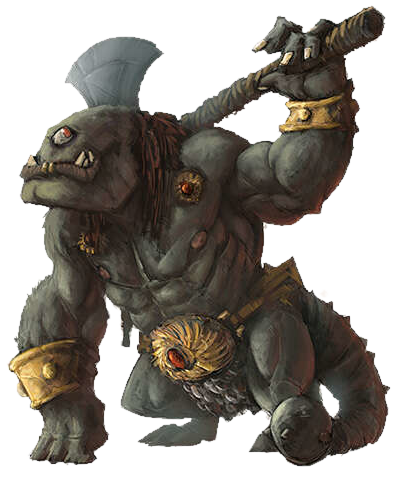
\includegraphics[width=0.47\textwidth]{03mechanics/img/31cyclops.png}
\end{figure}

\subsubsection{Damage Charts}
    \begin{DndTable}[width=\linewidth, header=Bludgeoning]{cX}
        \textbf{d20} & \textbf{Effect} \\
        1     & Roll damage as normal. \\
        2-3   & The next attack against the creature has advantage. \\
        4-6   & Push the creature up to 1.5 meters in any direction. \\
        7-8   & Push the creature up to 4.5 meters in any direction. \\
        9-11  & Attacks against the creature are made with advantage until the start of your next turn. \\
        12-13 & The creature is knocked prone. \\
        14-16 & Push the creature up to 4.5 meters away, and the creature is knocked prone. \\
        17-18 & Roll on the Minor Injury chart.
        If the creature is wearing heavy armor roll on the Major Injury chart instead. \\
        19    & Deal the twice maximum result of your damage dice and roll on the major injury chart. \\
        20    & Deal the maximum result of your damage dice twice, the creature is stunned until the end of your next turn, and roll on the major injury chart.
    \end{DndTable}

    \pagebreak

    \begin{DndTable}[width=\linewidth, header=Piercing]{cX}
        \textbf{d20} & \textbf{Effect} \\
        1     & Roll damage as normal. \\
        2-3   & The creature may only move half its movement speed on its next turn. \\
        4-6   & Roll damage dice twice and use the higher result. \\
        7-8   & The creature's movement speed is zero until the end of its next turn. \\
        9-11  & You can roll one of the weapon's damage dice one additional time and add it to the extra damage of the critical hit. \\
        12-13 & Roll on the minor injury chart with disadvantage. \\
        14-16 & Roll on the minor injury chart. \\
        17-18 & Roll on the major injury chart. \\
        19    & Roll on the major injury chart. \\
        20    & Roll on the minor injury chart, and roll on the major injury chart.
    \end{DndTable}

    \begin{DndTable}[width=\linewidth, header=Slashing]{cX}
        \textbf{d20} & \textbf{Effect} \\
        1     & Roll damage as normal. \\
        2-3   & The creature loses 1d6 hit points at the start of its next turn. \\
        4-6   & Choose one of the creature's arms or legs.
        If you slash one of its legs, its movement speed is halved until the end of its next turn.
        If you slash one of its arms, its attack rolls are made with disadvantage until the end of its next turn. \\
        7-8   & The creature is bleeding.
        For the next minute the creature loses 1d4 damage at the start of each of its turns until it uses two actions to staunch this wound. \\
        9-11  & Wounded, the creature has disadvantage on weapon attack rolls for a minute.
        The creature can roll a Constitution saving throw (DC 15) at the end of each of its turns.
        On a success, it ends this effect. \\
        12-13 & The creature is bleeding.
        For the next minute the creature loses 1d8 hit points at the start of each of its turns until it uses two actions to staunch this wound. \\
        14-16 & The creature is bleeding.
        For the next minute the creature loses 1d12 hit points at the start of each of its turns until it uses two actions to staunch this wound. \\
        17-18 & Roll on the minor injury chart.
        If the creature is wearing light or no armor roll on the major injury chart instead. \\
        19    & Roll on the major injury chart. \\
        20    & Roll on the major injury chart, and the creature is bleeding.
        For the next minute the creature loses 2d8 hit points at the start of each of its turns until it uses two actions to staunch this wound.
    \end{DndTable}

    \newpage

    \begin{DndTable}[width=\linewidth, header=Acid]{cX}
        \textbf{d20} & \textbf{Effect} \\
        1     & Roll damage as normal. \\
        2-3   & You induce temporary anosmia on the creature.
        While in this state, the creature has disadvantage on all Wisdom (Perception) checks that rely on smell.
        This counts as a minor injury. \\
        4-6   & The creature is scarred.
        While scarred the creature has disadvantage on all Charisma ability checks except Charisma (Intimidation).
        This counts as a minor injury. \\
        7-8   & You induce anosmia on the creature.
        While in this state, the creature automatically fails on all Wisdom (Perception) checks that rely on smell.
        Additionally, the creature has disadvantage on checks with Cooking Utensils.
        This counts as a major injury. \\
        9-11  & The creature is disfigured.
        While disfigured the creature has disadvantage on all Charisma ability checks except Charisma (Intimidation).
        This counts as a major injury. \\
        12-13 & The creature's AC is reduced by 1.
        If the creature is wearing armor, it must be repaired for 1/4th of the price of a new armor of the same type to regain its AC modifier.
        If not, this counts as a minor injury. \\
        14-16 & Roll on the minor injury chart.
        Additionally, the creature is disfigured.
        While disfigured the creature has disadvantage on all Charisma ability checks except Charisma (Intimidation).
        This counts as a major injury. \\
        17-18 & The creature's AC is reduced by 2.
        If the creature is wearing armor, it must be repaired for half of the price of a new armor of the same type to regain its AC modifier.
        If not, this counts as a minor injury. \\
        19    & Roll on the major injury chart. \\
        20    & If the creature is wearing armor, the armor is destroyed and roll on the major injury chart.
        If the creature is not wearing armor, roll on the major injury chart and the creature is disfigured.
        While disfigured the creature has disadvantage on all Charisma ability checks except Charisma (Intimidation).
        This counts as a major injury.
    \end{DndTable}

    \thispagestyle{empty} % Remove footer so that it doesn't clash with the image.
    \begin{tikzpicture}[remember picture,overlay]
        \node[anchor=south east, xshift=0.10cm, yshift=-0.10cm] at (current page.south east) {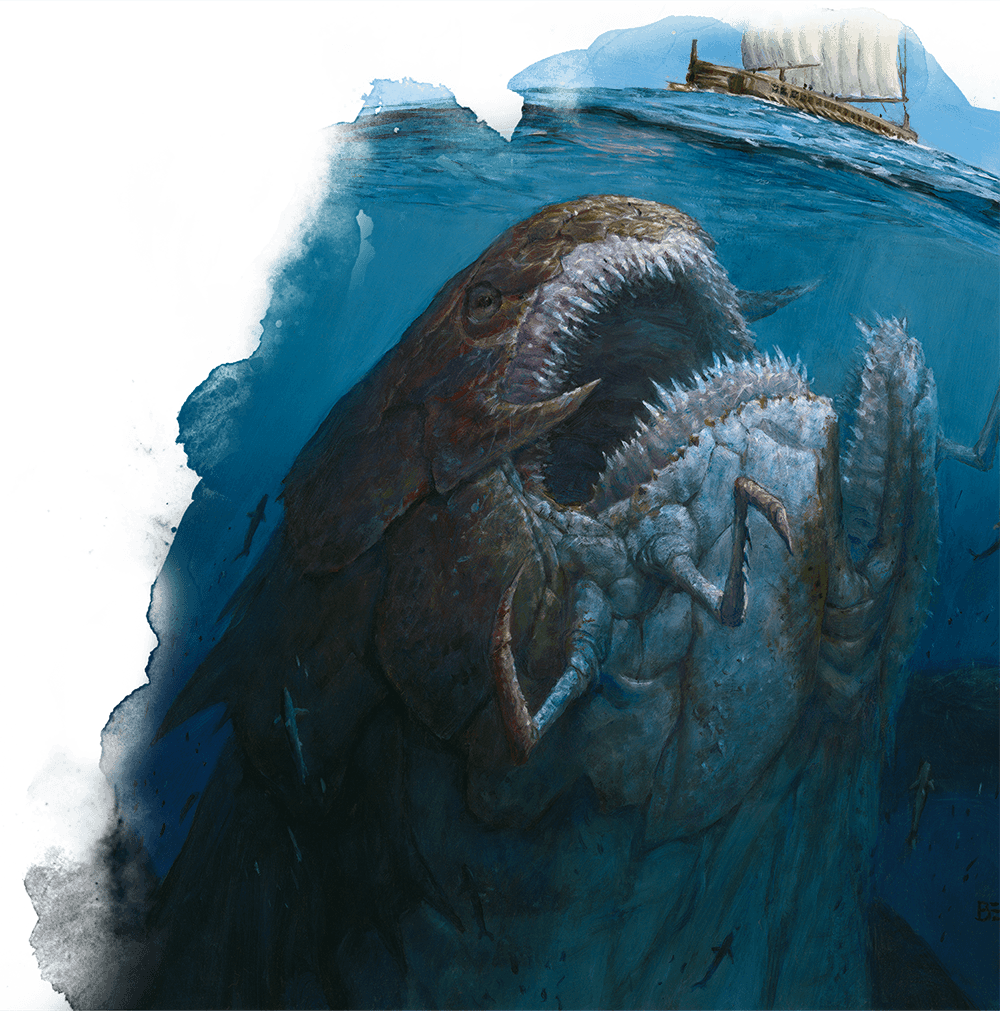
\includegraphics[width=0.5\pdfpagewidth]{03mechanics/img/31friendlyillhevi.png}};
    \end{tikzpicture}

    \newpage

    \begin{DndTable}[width=\linewidth, header=Cold]{cX}
        \textbf{d20} & \textbf{Effect} \\
        1     & Roll damage as normal. \\
        2-3   & The creature may only move half its movement speed on its next turn. \\
        4-6   & The creature has disadvantage on attack rolls until the end of its next turn. \\
        7-8   & The creature’s movement speed is 0 until the end of its next turn. \\
        9-11  & The creature gains vulnerability to bludgeoning damage for a minute. \\
        12-13 & The creature is paralyzed until the end of its next turn. \\
        14-16 & The creature is paralyzed until the end of its next turn.
        If the creature takes damage before the end of its next turn, roll on the minor injury chart. \\
        17-18 & The creature is paralyzed until the end of its next turn and rolls on the minor injury chart. \\
        19    & Roll on the major injury chart. \\
        20    & Roll on the major injury chart, and the creature is paralyzed for the next minute.
        The creature may attempt a Constitution saving throw at the end of each of its turns (DC 15) to end this effect.
        If it fails this saving throw three times it is frozen solid and becomes petrified, but frozen solid rather than turned to stone.
    \end{DndTable}

    \begin{DndTable}[width=\linewidth, header=Fire]{cX}
        \textbf{d20} & \textbf{Effect} \\
        1     & Roll damage as normal. \\
        2-3   & Attack rolls for attacks that deal fire damage have advantage against the creature until the end of its next turn. \\
        4-6   & You burn the creature's hands.
        The creature drops any objects it is holding. \\
        7-8   & The creature is on fire.
        While the creature is on fire it takes 2d4 fire damage at the start of each of its turns.
        The creature can end this condition by dropping prone and using 1.5 meters of movement to roll on the ground. \\
        9-11  &  \\
        12-13 & The creature is on fire.
        While the creature is on fire it takes 2d6 fire damage at the start of each of its turns.
        The creature can end this condition by dropping prone and using 1.5 meters of movement to roll on the ground. \\
        14-16 & The creature is charred.
        If the creature has resistance to fire, it loses that resistance.
        If the creature does not have resistance to fire, it gains vulnerability to fire.
        Both of these effects are considered a minor injury. \\
        17-18 & Roll on the minor injury chart.
        Additionally, the creature is on fire.
        While on fire it takes 2d6 fire damage at the start of each of its turns.
        The creature can end this condition by dropping prone and using 1.5 meters of movement to roll on the ground. \\
        19    & Roll on the major injury chart. \\
        20    & Roll on the major injury chart.
        Additionally, the creature is on fire.
        While the creature is on fire it takes 2d8 fire damage at the start of each of its turns.
        The creature can end this condition by dropping prone and using 1.5 meters of movement to roll on the ground.
    \end{DndTable}

    \begin{DndTable}[width=\linewidth, header=Force]{cX}
        % TODO: Check back here after done with spells. Dunno if we're keeping Force damage.
        \textbf{d20} & \textbf{Effect} \\
        1     & Roll damage as normal. \\
        2-3   & The creature has disadvantage on saving throws against spells until the end of its next turn. \\
        4-6   & The creature is pushed 4.5 meters away from you. \\
        7-8   & Spell attack rolls against the creature have advantage until the end of its next turn. \\
        9-11  & The creature is knocked prone. \\
        12-13 & The creature is spellbound until the end of its next turn.
        While spellbound it makes saving throws against spells with disadvantage and spell attack rolls against it have advantage. \\
        14-16 & The creature is spellbound for the next minute.
        While spellbound it makes saving throws against spells with disadvantage and spell attack rolls against it have advantage.
        At the end of each of the creature’s turns it can make an Intelligence saving throw (DC 12) to end this effect. \\
        17-18 & Roll on the minor injury chart.
        Additionally, the creature is spellbound for the next minute.
        While spellbound it makes saving throws against spells with disadvantage and spell attack rolls against it have advantage.
        At the end of each of the creature’s turns it can make an Intelligence saving throw (DC 15) to end this effect. \\
        19    & Roll on the major injury chart. \\
        20    & Roll on the major injury chart.
        Additionally, the creature is spellbound for the next minute.
        While spellbound it makes saving throws against spells with disadvantage and spell attack rolls against it have advantage.
        At the end of each of the creature’s turns it can make an Intelligence saving throw (DC 18) to end this effect.
    \end{DndTable}

    \begin{DndTable}[width=\linewidth, header=Lightning]{cX}
        \textbf{d20} & \textbf{Effect} \\
        1     & Roll damage as normal. \\
        2-3   & The creature cannot use reactions until the end of its next turn. \\
        4-6   & If the creature willingly moves before the start of your next turn, it takes 1d8 lightning damage. \\
        7-8   & You may choose one other creature within 4.5 m. of the victim.
        That creature must succeed on a Dexterity saving throw (DC 12) or take half as much damage. \\
        9-11  & The creature is paralyzed until the start of your next turn. \\
        12-13 & You may choose one other creature within 4.5 m. of the victim.
        That creature must succeed on a Dexterity saving throw (DC 15) or take half as much damage. \\
        14-16 & Roll on the minor injury chart.
        If the creature is wearing metal armor roll on the major injury chart instead. \\
        17-18 & The creature and all creatures within 4.5 m. of it cannot take reactions until the end of their next turn.
        Then roll on the minor injury chart. \\
        19    & Roll on the major injury chart. \\
        20    & All creatures within 4.5 m. of the victim must succeed on a Dexterity saving throw (DC 18) or take half as much damage.
        Then roll on the major injury chart.
    \end{DndTable}

    \begin{DndTable}[width=\linewidth, header=Necrotic]{cX}
        \textbf{d20} & \textbf{Effect} \\
        1     & Roll damage as normal. \\
        2-3   & The creature cannot regain hit points until the end of its next turn. \\
        4-6   & Choose an ability.
        The creature has disadvantage on ability checks made with the chosen ability for a minute. \\
        7-8   & The creature’s maximum hit points are reduced by an amount equal to the damage dealt.
        This lasts until the creature takes a short rest. \\
        9-11  & You heal yourself an amount equal to half of the damage dealt. \\
        12-13 & The creature’s maximum hit points are reduced by an amount equal to the damage dealt.
        This is considered a minor injury. \\
        14-16 & The creature cannot regain hit points for the next minute.
        It may make a Constitution saving throw (DC 15) at the end of each of its turns to end this effect. \\
        17-18 & The creature’s maximum hit points are reduced by an amount equal to the damage dealt.
        This is considered a major injury.
        Then roll on the minor injury chart. \\
        19    & Roll on the major injury chart. \\
        20    & The creature cannot regain hit points for the next minute.
        It may make a Constitution saving throw (DC 18) at the end of each of its turns to end this effect.
        Then roll on the major injury chart.
    \end{DndTable}

    \begin{DndTable}[width=\linewidth, header=Poison]{cX}
        \textbf{d20} & \textbf{Effect} \\
        1     & Roll damage as normal. \\
        2-3   & The creature has disadvantage on its next ability check, attack roll, or saving throw. \\
        4-6   & The creature stinks.
        It has disadvantage on all Charisma checks except Charisma (Intimidation) and Perception checks that rely on smell.
        This lasts until the creature bathes. \\
        7-8   & The creature has disadvantage on all ability checks, attack rolls, and saving throws until the end of its next turn. \\
        9-11  & Any creature in a radius of 3 meters around the target must roll a Constitution saving throw.
        On a failure, they take half the damage dealt. \\
        12-13 & The creature is poisoned for the next minute.
        The creature may attempt a Constitution saving throw at the end of each of its turns (DC 12) to end this effect. \\
        14-16 & The creature is poisoned for the next minute.
        The creature may attempt a Constitution saving throw at the end of each of its turns (DC 15) to end this effect. \\
        17-18 & Roll on the minor injury chart and the creature is poisoned for the next minute.
        The creature may attempt a Constitution saving throw at the end of each of its turns (DC 18) to end this effect. \\
        19    & Roll on the major injury chart. \\
        20    & Roll on the major injury chart, and the creature is poisoned for the next minute.
        The creature may attempt a saving throw at the end of each of its turns (DC 18) to end this effect.
    \end{DndTable}

    \begin{DndTable}[width=\linewidth, header=Psychic]{cX}
        \textbf{d20} & \textbf{Effect} \\
        1     & Roll damage as normal. \\
        2-3   & You control the creature’s movement on its next turn. \\
        4-6   & The creature cannot differentiate friend from foe until the end of its next turn. \\
        7-8   & Attacks against the creature are made with advantage until the start of your next turn. \\
        9-11  & You control the creature’s actions on its next turn. \\
        12-13 & The creature's mind is broken.
        If the creature has resistance to psychic damage, it loses that resistance.
        If the creature does not have resistance to psychic damage, it gains vulnerability to it.
        Both of these effects are considered a minor injury. \\
        14-16 & You control the creature during its next turn. \\
        17-18 & Roll on the Insanity chart with disadvantage. \\
        19    & Roll on the Insanity chart. \\
        20    & Roll on the Insanity chart with advantage.
    \end{DndTable}

    \begin{DndTable}[width=\linewidth, header=Radiant]{cX}
        \textbf{d20} & \textbf{Effect} \\
        1     & Roll damage as normal. \\
        2-3   & The has disadvantage on any Perception checks that rely on sight.
        This is considered a minor injury. \\
        4-6   & The creature's attack rolls are made with disadvantage. \\
        7-8   & The creature is blinded until the end of its next turn. \\
        9-11  & The creature is blinded for a minute.
        It can make a Constitution saving throw (DC 12) at the end of each of its turns to end this effect. \\
        12-13 & The creature glows for the next minute.
        While glowing it produces bright light up 3 meters and dim light up to 9 meters and all successful attacks against the creature deal an additional 1 radiant damage. \\
        14-16 & The creature is frightened of you for the next minute.
        It can make a Wisdom saving throw (DC 15) at the end of each of its turns to end this effect. \\
        17-18 & Roll on the minor injury chart.
        Additionally, the creature glows for the next minute.
        While glowing it produces bright light up 3 meters and dim light up to 9 meters and all successful attacks against the creature deal an additional 1d4 radiant damage. \\
        19    & Roll on the major injury chart. \\
        20    & Roll on the major injury chart.
        Additionally, the creature glows for the next minute.
        While glowing it produces bright light up 3 meters and dim light up to 9 meters and all successful attacks against the creature deal an additional 1d6 radiant damage.
    \end{DndTable}

    \pagebreak~
    \begin{tikzpicture}[remember picture,overlay]
        \node[anchor=north, yshift=0.10cm] at (current page.north) {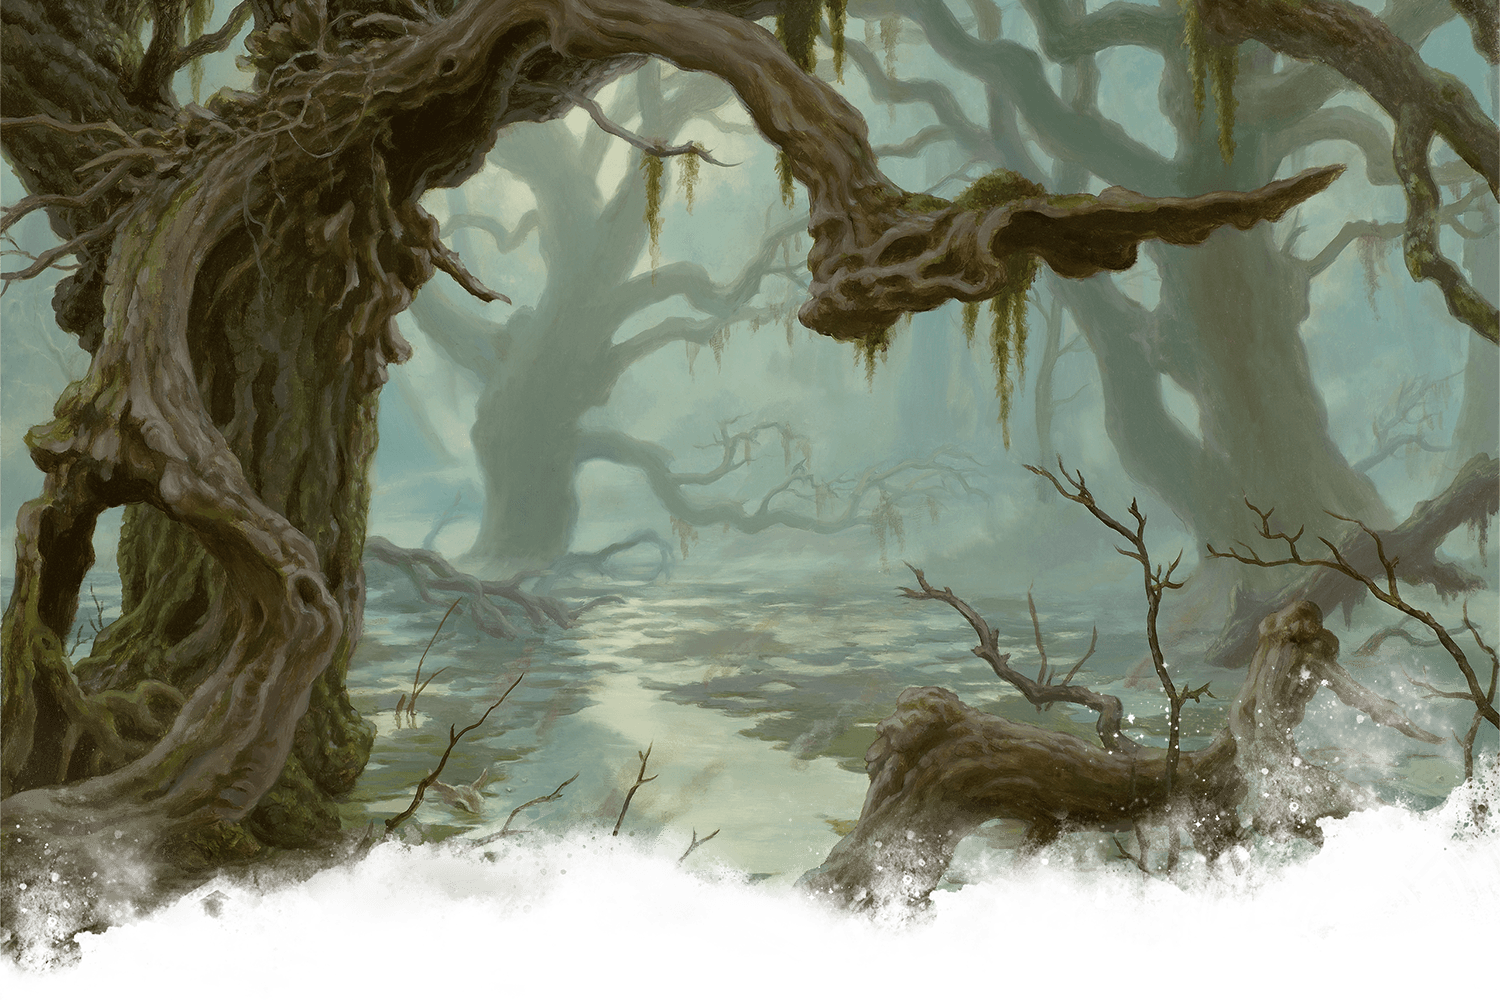
\includegraphics[width=\pdfpagewidth]{03mechanics/img/31arastas_domain.png}};
    \end{tikzpicture}

    \vspace{12.0cm}

    \begin{DndTable}[width=\linewidth, header=Thunder]{cX}
        \textbf{d20} & \textbf{Effect} \\
        1     & Roll damage as normal. \\
        2-3   & The creature has disadvantage on any Perception checks that rely on hearing.
        This is considered a minor injury. \\
        4-6   & The creature is deafened until the end of its next turn. \\
        7-8   & The creature is confused until the end of its next turn.
        While confused, the creature moves in a random direction determined by the DM. \\
        9-11  & The creature is deafened for one minute. \\
        12-13 & The creature is stunned until the start of its next turn and is deafened for one minute. \\
        14-16 & The creature is deafened permanently.
        This is considered a major injury. \\
        17-18 & The creature is stunned until the end of its next turn and is deafened for one minute.
        Then roll on the minor injury chart. \\
        19    & Roll on the major injury chart. \\
        20    & The creature is stunned until the end of its next round and is deafened for one minute.
        Then roll on the major injury chart.
    \end{DndTable}

% !TEX root = ../main.tex

\pagebreak~
\vspace{11.5cm}

\subsection*{Dementia} \label{ssec::dementia}
\DndDropCapLine{H}{arsh is the process that awaits the}
foolish or unlucky enough to lose their qualar.
Their sentience slips away slowly as they lose their mental capacities.
Perhaps the worst part is that inward awareness is one of the last attributes lost, forcing them to be fully conscious of the process.

The road towards dementia comes in seven stages, each roughly lasting a week.
At the moment when you lose your qualar, you enter the first stage of dementia.
After a week, you roll a DC 15 Intelligence saving throw.
On a fail, you enter the next stage of dementia.
On a success, you stay on your current stage and roll again at the start of the next week.
Dementia is unavoidable, and the DC increases by 1 after every successful roll.

\subsubsection{First Stage}
    No obvious signs of dementia, only minor short-memory loss occurs.
    The main symptoms are associated to the anxiety from the loss of the qualar.
    You start focusing more on your past, often drifting away into daydreams.

    You suffer the following effects:
    \subparagraph{Decreased Awareness} You roll for initiative and Dexterity saving throws with disadvantage.
    \subparagraph{Restlessness} Roll an DC 12 intelligence saving throw right after a short rest.
    On a success, you recover your hit points normally.
    On a failure, you only recover half of the hit dice rolled (rounded down).

\subsubsection{Second Stage}
    The self realization and awareness that something is wrong settles in.
    You refuse to accept that your mind is slipping away.
    The more effort you put on remembering the more deterioration your memory suffers.
    Confusion starts setting in.

    In addition to the effects of the first stage, you suffer the following effects:
    \subparagraph{Lack of Recollection} Any ability check made to remember or recollect a memory is done with disadvantage.
    All Intelligence (History) checks are made with disadvantage.
    \subparagraph{Mood Swings} All Charisma ability checks and saving throws are made with disadvantage.

\subsubsection{Third Stage}
    You experience increased forgetfulness and might find concentrating difficult.
    You are presented with some of the last coherent memories before confusion fully rolls in.
    Some singular memories become more disturbed, isolated, broken, and distant.
    These are the last embers of awareness.

    In addition to the effects of the last stages, you suffer the following effects:
    \subparagraph{Decreased Concentration} All Constitution saving throws made to maintain concentration are made with disadvantage.
    \subparagraph{Vagrant Mind} Intelligence and Wisdom ability checks and saving throws are rolled with disadvantage.

\subsubsection{Fourth Stage}
    Grey mists form and fade away in your memory.
    The ability to recall singular memories gives way to confusion and horror.
    You struggle with daily tasks, presenting clear cognitive problems.

    In addition to the effects of the last stages, you suffer the following effects:
    \subparagraph{Motor Difficulties} Strength and Dexterity ability checks and saving throws are rolled with disadvantage.
    Attack rolls are made with disadvantage.
    \subparagraph{Drifting Conscience} In combat, roll a DC 8 Intelligence saving throw at the start of every turn.
    On a failure, you forget where you are, and cannot take any actions during the turn.

\subsubsection{Fifth Stage}
    You have major memory deficiencies.
    The few lapses of consciousness you get are filled with dread, as you realize your mind has mostly left you.
    The repetition and rupture gives way to calmer moments, as the unfamiliar becomes familiar.

    In addition to the effects of the last stages, you suffer the following effects:
    \subparagraph{Loss of Fortitude} All rolls are made with disadvantage.
    \subparagraph{Complete Unawareness} All Intelligence (Investigation), Wisdom (Insight), and Wisdom (Perception) automatically fail.
    Your passive investigation, insight, and perception become 0.

\subsubsection{Sixth Stage}
    Your mental state is beyond description.
    You struggle to remember your early life, even forgetting the names of your family and fellows.
    Your capacity of speech is severely impaired, and you suffer sudden and radical personality and emotional changes.

    In addition to the effects of the last stages, you suffer the following effects:
    \subparagraph{Declining Speech} You automatically fail all Charisma ability checks and saving throws, and have a very hard time communicating verbally.
    \subparagraph{Hope Lost} As your conscious mind fights your natural tendencies, you automatically fail death saving throws.

\subsubsection{Final Stage}
    Everywhere, an empty bliss.

    You make what will most likely be your last die roll.
    Nothing can give you advantage or disadvantage on this roll.
    Roll a d20 on the post-dementia table.
    You suffer the effect rolled.

    \begin{DndTable}[width=\linewidth, header=Post-dementia Effects]{lX}
        \textbf{Roll} & \textbf{Effect} \\
        1 & Your last emotion is rage.
        You become mindless and violent, attacking your companions without reason. \\
        2-5 & Your last emotion is apathy.
        You mindlessly stare to the east until you die of natural causes. \\
        6-18 & Even after brain death, you seek survival.
        You wander off, attacking any who try to stop you.
        You become a lost one. \\
        19 & With memories gone, your mind is fully pulled by its tidal impulses.
        You lose control of your character, who becomes a servant of The Sorrow. \\
        20 & Recovery from dementia is very rare, but not impossible.
        You recover from all effects associated to dementia, and gain the \textbf{Demented Insight} feat at page \pageref{feat::dementedinsight}.
    \end{DndTable}

    The only conventional way to remove dementia is to obtain a qualar again.
    When this happens, you quickly recover your sentience.
    Each morning, you reduce your stage of dementia by one, and don't need to roll the Intelligence saving throw associated to the status.


% \subsection*{Encumbrance} \label{ssec::encumbrance}
%     \textbf{TODO.}
% NOTE: We can stay with vanilla's system, it's good enough tbh.

\pagebreak~
\begin{tikzpicture}[remember picture,overlay]
    \node[anchor=north, yshift=0.10cm] at (current page.north) {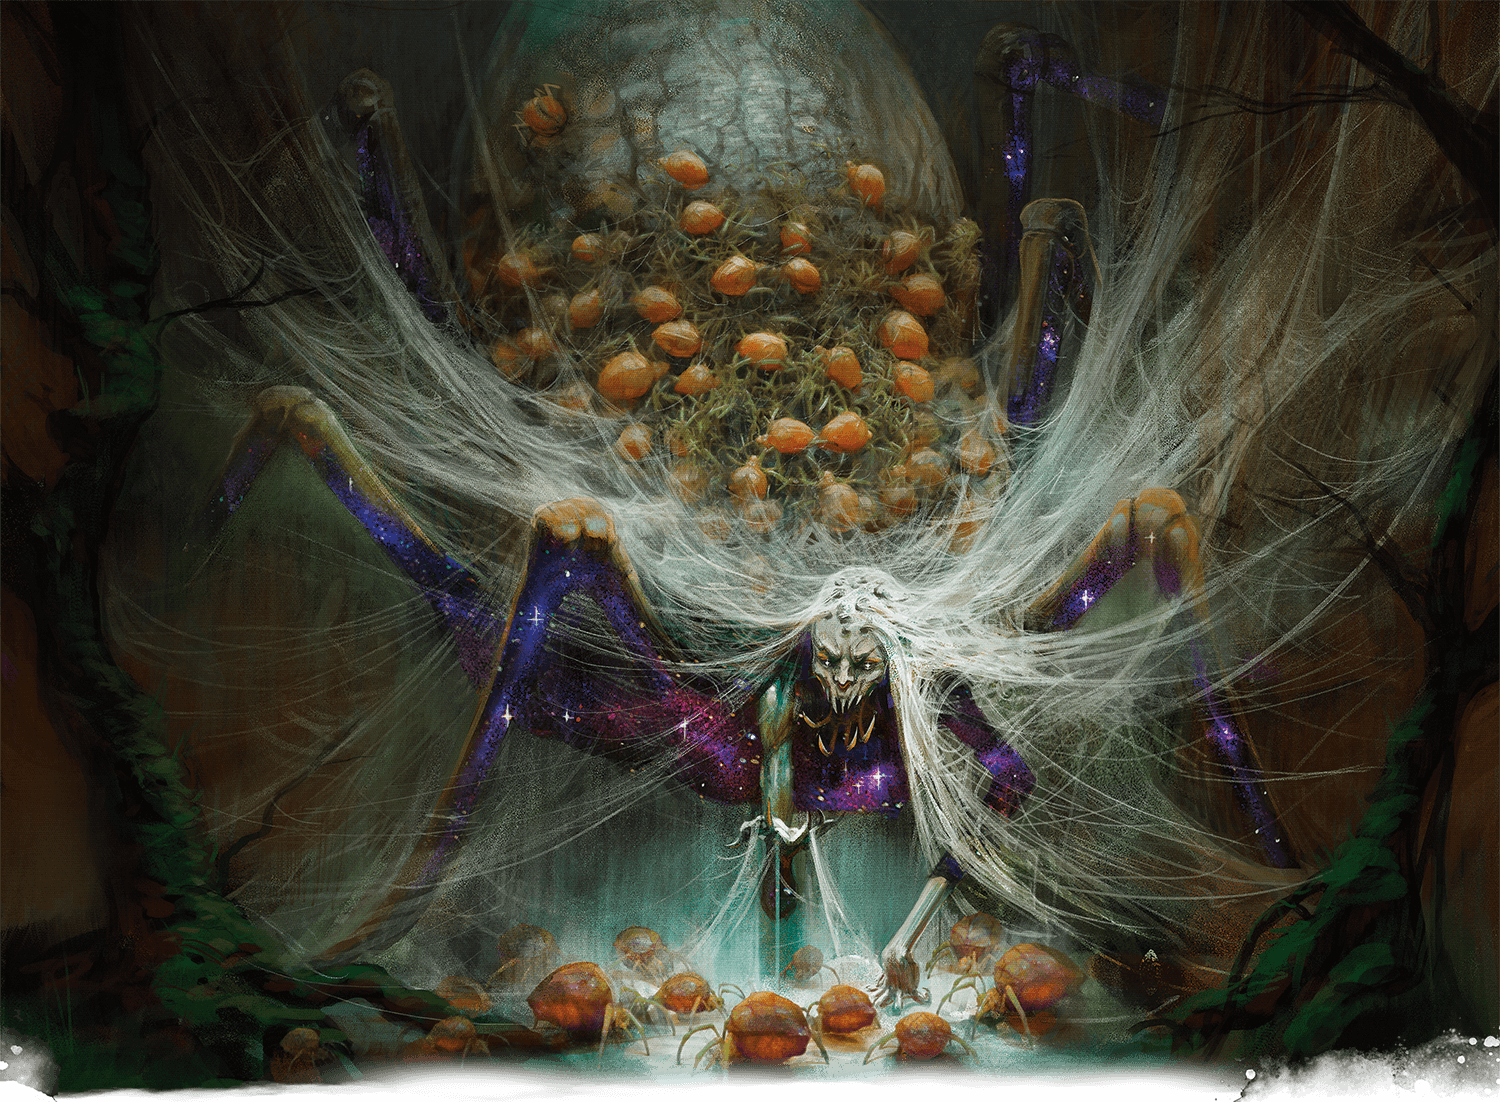
\includegraphics[width=\pdfpagewidth]{03mechanics/img/30arastaoftheendlessweb.png}};
\end{tikzpicture}

\vspace{14.0cm}

\subsection*{Flaws} \label{ssec::flaws}
    As you travel through treacherous lands and fight dangerous creatures, it is natural to acquire permanent wounds or fears.
    These new flaws don't need to be entirely bad --- they reflect a changing point in your life, and can be beneficial in their own way.

    When you suffer a major injury, fear, or insanity, you can choose to accept this effect as a flaw.
    When you do so, it becomes permanent.
    For example, a crippled arm might need to be severed off, or your character might get used to their insanity and learn to live with it instead of treating it.

    While this effect may prove as a permanent hindrance to you, you are rewarded with FP for taking it.
    This extra FP does not count towards your level.
    The number of FP awarded by effects is specified in the effect's description.

% \subsection*{Hunger and Thirst} \label{ssec::hungerandthirst}
%     \textbf{TODO.}
% NOTE: We can stay with vanilla's system, it's good enough tbh.

\pagebreak~
\vspace{11.5cm}

\subsection*{Injuries \& Insanity} \label{ssec::injuriesandinsanity}
    Critical hits or especially severe events can cause injuries or insanity.
    When a creature suffers a minor injury it can be healed by someone competent with a healer's kit over the course of a long rest.
    Major injuries and Insanities require assistance from a dedicated healer, or someone with the relevant feat (see page \pageref{feat::physician} and \pageref{feat::therapist}).

    Alternatively, you can decide to keep an injury or insanity as a new Flaw (see page \pageref{ssec::flaws}) during a short rest after it is applied.
    Minor injuries and insanities award you 2 FP, while major injuries award you 3 FP.
    Acquiring a flaw from a major injury related to a minor injury you already have (such as Crippled Leg and Injured Leg) only awards 1 FP --- one more than what you already had gained.
    % The text of certain injuries will specify other ways this injuries might resolve.

    \pagebreak

    \begin{table*}[t]
        \begin{DndTable}[width=\linewidth, header=Minor and Major Injuries]{cXX}
            \textbf{d20} & \textbf{Minor Injury} & \textbf{Major Injury} \\
            1-3 &
            \textbf{Injured leg}.
            Your movement speed is reduced by 2 meters. &
            \textbf{Crippled leg}.
            Your movement speed is reduced by 2 meters, and you have disadvantage on Dexterity saving throws. \\
            4-8 &
            \textbf{Injured arm}.
            One of your arms (randomly determined) cannot be used to hold a shield, and you have disadvantage on any rolls involving the use of that arm. &
            \textbf{Crippled arm}.
            One of your arms (randomly determined) cannot be used to hold an item, and any ability check or attack roll requiring that arm automatically fails. \\
            9-11 &
            \textbf{Multiple injuries}.
            Your maximum hitpoints are reduced by an amount equal to half of the damage dealt by the attack. &
            \textbf{Severely wounded}.
            Your maximum hit points are reduced by an amount equal to the damage dealt by the attack. \\
            12-16 &
            \textbf{Badly beaten}.
            You have disadvantage on Constitution saving throws. &
            \textbf{Edge of death}.
            You have disadvantage on Constitution and death saving throws. \\
            17-19 &
            \textbf{Ringing blow}.
            You are stunned until the end of your next turn, and you are deafened. &
            \textbf{Blinding blow}.
            You are blinded. \\
            20    &
            \textbf{Blow to the head}
            You are unconscious for 2d12 hours. &
            \textbf{Decapitated}.
            You are dead.
        \end{DndTable}
    \end{table*}

    \thispagestyle{empty} % Remove footer so that it doesn't clash with the image.
    \begin{tikzpicture}[remember picture,overlay]
        \node[anchor=south west, xshift=-0.10cm, yshift=-0.10cm] at (current page.south west) {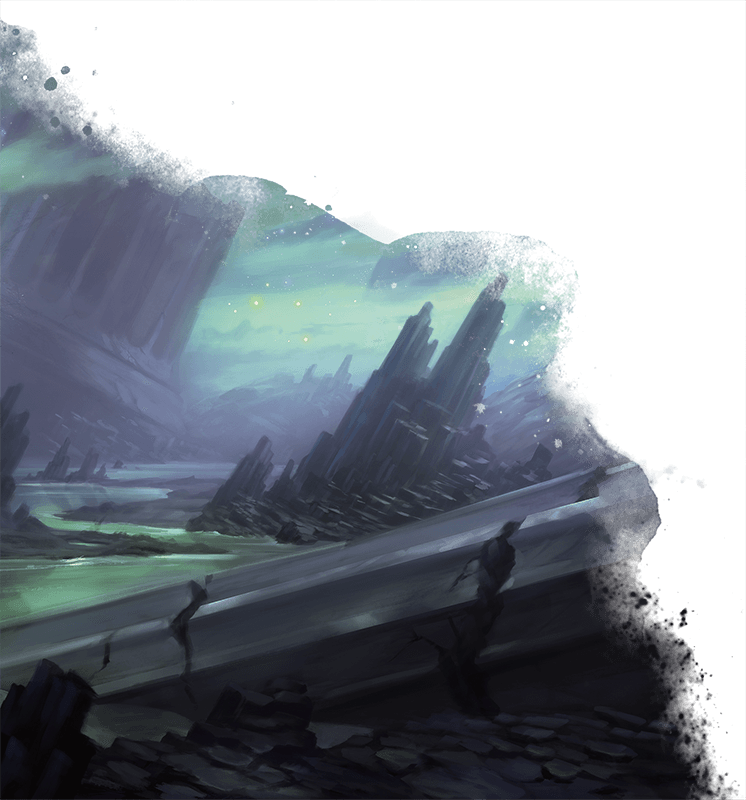
\includegraphics[width=0.5\pdfpagewidth]{03mechanics/img/30outerlands.png}};
    \end{tikzpicture}

\subsection*{Only One Chance} \label{ssec::onlyonechance}
    As a rule, you only have one chance to succeed in any action.
    Once you have rolled the dice, you many not roll again to achieve the same goal.
    You need to try something different or wait until the circumstances have changed in a substantial way.
    Or, you know, let another PC try.

    This rule does not apply to combat, where you can attack the same enemy until it becomes a bloody pulp.

\subsection*{Opportunity Attacks} \label{rule::opportunityattacks}
    In a fight, everyone is constantly watching for enemies to drop their guard.
    While heedless movement is easily punished, any lack of concentration or unplanned action can have devastating consequences.
    Various actions provoke opportunity attacks from a creature:
    \begin{itemize}
        \item Moving out of the creature's reach.
        This doesn't apply when someone or something moves you without using your movement, action, or reaction.

        \newpage

        \item Picking up an item from the floor while in the creature's reach.
        \item Unsheathing a weapon while in the creature's reach.
        \item Donning or doffing a shield while in the creature's reach.
        \item Using the Attack action with a ranged weapon or spell attack in a creature's reach.
    \end{itemize}
    You can avoid opportunity attacks during your turn by taking the Disengage action.

\subsection*{Short and Long Rests} \label{ssec::shortandlongrests}
    The gritty campaigns in Yuadrem benefit from longer rest times.
    Short rests last for 8 hours, and long rests for 3 days --- half a week in the Fagalian calendar.
    This puts the brakes on the campaign, requiring the players to carefully judge the benefits and drawbacks of combat.
    % Characters can't afford to engage in too many battles in a row, and all adventuring requires careful planning.

    Complementing this optional rule is the fact that all spell slots are recovered during short rests, and a short rest removes one level of exhaustion.
    Additionally, all the systems in this book are designed with this optional rule in mind, so some things need to be re-balanced if a group is to play without this rule.

    \begin{table*}[h]
        \begin{DndTable}[width=\linewidth, header=Insanity]{cX}
            \textbf{d20} & \textbf{Insanity} \\
            1  & \textbf{Synesthesia}.
            You can hear colors, smell sounds, or taste textures. Regardless of the specific manifestation, you have disadvantage on all Perception and Investigation skill checks. \\
            2  & \textbf{Kleptomania}.
            Once per day when you are in a personal residence or marketplace, the DM can call on you to succeed on a Wisdom saving throw (DC 12) or attempt to steal an item of insignificant practical and monetary value. \\
            3  & \textbf{Paranoia}.
            Once per day following an interaction with another creature (including other PCs) the DM can call on you to succeed on a Wisdom saving throw (DC 12) or you suspect that creature is secretly plotting against you. \\
            4  & \textbf{Obsession}.
            Choose a person or personal interest you are obsessed with. Once per day, when you are presented with an opportunity to interact with or learn more about the subject of your obsession the DM can call on you to succeed on a Wisdom saving throw (DC 14) or ignore everything else to obsess over the object of your fascination. \\
            5  & \textbf{Addiction}.
            Choose a behavior or substance you have used. Once per day, when you are presented with an opportunity to do the behavior or use the substance the DM can call on you to succeed on a Wisdom saving throw (DC 14) or ignore everything else to indulge in your vice. \\
            6  & \textbf{Odd Thinking}.
            Once per day when you hear a rational explanation for an event or occurrence, your DM may call on you to succeed on a Wisdom saving throw (DC 12) or you reject the rational explanation for a conspiratorial or fantastical explanation. \\
            7  & \textbf{Narcissism}.
            When you take an action or series of action that doesn’t directly benefit you, you must pass a Wisdom saving throw (DC 11) or you can’t take that action / series of actions.
            If any self-sacrifice on your part would be required the DC of the saving throw is increased to 16. \\
            8  & \textbf{Delusional}.
            When you gain this insanity the DM will tell you a belief that you have. No matter what evidence is presented to the contrary so long as you have this insanity you cannot be persuaded that this belief is not true. \\
            9  & \textbf{Pica}.
            Once per day the DM can call on you to pass a Wisdom saving throw (DC 14) or immediately eat one non-food object (such as dirt, napkins, or a small piece of jewelry) of the DM’s choice. \\
            10 & \textbf{Retrograde amnesia}.
            You forget everything about your personal life prior to the moment you received this insanity. \\
            11 & \textbf{Overwhelmed}.
            If you do not have immunity or resistance to psychic damage, you gain vulnerability to psychic damage.
            If you have resistance to psychic damage, you lose it.
            If you have immunity to psychic damage, you lose it but gain resistance to psychic damage. \\
            12 & \textbf{Anterograde amnesia}.
            Whenever you try to recall a fact you learned since you received this insanity, make a Intelligence saving throw (DC 12).
            If you fail you cannot recall the fact. \\
            13 & \textbf{Dependence}.
            You must pass a Wisdom saving throw (DC 14) to take an action that one or more of your allies disapprove of. \\
            14 & \textbf{Anxious}.
            You have disadvantage on saving throws against being frightened.
            Additionally, once per day the DM can call on you to succeed a Wisdom saving throw (DC 14) or be frightened by a creature of the DM’s choosing for the next minute. \\
            15 & \textbf{Mute}.
            Whenever you wish to speak allowed (including casting a spell that has verbal components) you must succeed on a Wisdom saving throw (DC 13) to do so. \\
            16 & \textbf{Narcolepsy}.
            You have disadvantage on saving throws against sleeping or unconsciousness.
            Once per day the DM may call on you to succeed on a Constitution saving throw (DC 12) or fall unconscious for one minute or until you take damage or another creature spends their action trying to rouse you. \\
            17 & \textbf{Insomnia}.
            You cannot take long rests and your short rests take 8 hours to complete. \\
            18 & \textbf{Homicidal}.
            After each long rest you must pass a Wisdom saving throw (DC 14) or be overcome with the urge to end the life of a humanoid creature and you cannot benefit from another long rest until you do so. \\
            19 & \textbf{Suicidal}.
            After each long rest you must pass a Wisdom saving throw (DC 12) or make an attempt to end your own life. \\
            20 & \textbf{Catatonia}.
            You are unconscious for 10d10 years.
        \end{DndTable}
    \end{table*}

\subsection*{Stress} \label{ssec::stress}
    Adventuring is dangerous, and no matter the amount of heroic deeds in your past you are bound to accumulate stress over time.
    As a mechanic, stress adds long-term consequences to traumatic experiences and tense situations.

    Whenever you drop to 0 hit points, add a point to your stress meter.
    % Some specific attacks directly produce stress on a creature.
    When you reach 4 stress points, you roll on the Afflictions table and acquire the specified affliction, reducing your stress meter back to 2.
    % Afflictions are detrimental conditions that have short or long-term consequences for you.

    Taking a long rest or engaging in downtime activities reduces your stress meter by 1.
    Additionally, some feats like Soothing Presence (see page \pageref{feat::soothingpresence}) and Reliever (see page \pageref{feat::reliever}) add the capacity to reduce stress in different scenarios.

    \newpage~\newpage~\newpage

    \begin{table*}[t]
    \begin{DndTable}[width=\linewidth, header=Affliction]{cX}
        \textbf{d20} & \textbf{Affliction} \\
        1     & \textbf{Insanity}.
        Your mind collapses and you fall into insanity.
        Roll on the Insanity table (see page \pageref{ssec::injuriesandinsanity}) and acquire the rolled insanity. \\
        2-5   & \textbf{Phobia}.
        Powerless at the face of death, you can only watch as your foe strikes its final blow against you.
        You add to your flaws the phobia of the type of creature who put you unconscious.
        Any time you encounter this type of creature, roll a DC 16 Wisdom saving throw at the beginning of each of your turns.
        On a failure, you become frightened of the creature.
        This flaw is permanent, and awards you 1 FP. \\
        6-7   & \textbf{Fearful}.
        % Scared of death, you become fearful and meek.
        Whenever you take damage, roll a DC 12 Wisdom saving throw.
        On a failure, you become frightened of the attacking creature.
        You can repeat this saving throw at the end of each turn.
        This effect lasts until you finish a short rest. \\
        8-9   & \textbf{Paranoid}.
        Whenever you are targetted by a friendly creature for any effect, roll a DC 12 Wisdom saving throw.
        On a failure, you refuse what your ally is offering, be it healing, aid, etc.
        If you ally spent any resource or action on this effect, they are spent anyway.
        This effect lasts until you finish a short rest. \\
        10-11 & \textbf{Selfish}.
        You cannot heal or aid an ally in any way.
        This effect lasts until you finish a short rest. \\
        12-13 & \textbf{Masochistic}.
        Your AC is reduced by 2, and you cannot take the Dodge or Disengage actions.
        This effect lasts until you finish a short rest. \\
        14-15 & \textbf{Abusive}.
        You cannot heal or aid an ally in any way, and you refuse to receive any healing or aid from any creature.
        This effect lasts until you finish a short rest. \\
        16-17 & \textbf{Hopeless}.
        Attacks against you are made with advantage, and you roll saving throws with disadvantage.
        This effect lasts until you finish a short rest. \\
        18-19 & \textbf{Irrational}.
        At the beginning of each of your turns, roll a DC 15 Wisdom saving throw.
        On a failure, you cannot take any action during your turn.
        This effect lasts until you finish a short rest. \\
        20    & \textbf{Virtuous}.
        Stalwart against adversity, your time at death's door only enhances your resolution.
        Your stress meter is reduced to 0, and any ally that can see or hear you has their stress meter reduced by 1.
        Additionally, you have advantage on attack rolls and saving throws for one hour.
    \end{DndTable}
    \end{table*}

    \thispagestyle{empty}
    \begin{tikzpicture}[remember picture,overlay]
        \node[anchor=south, yshift=-0.10cm] at (current page.south) {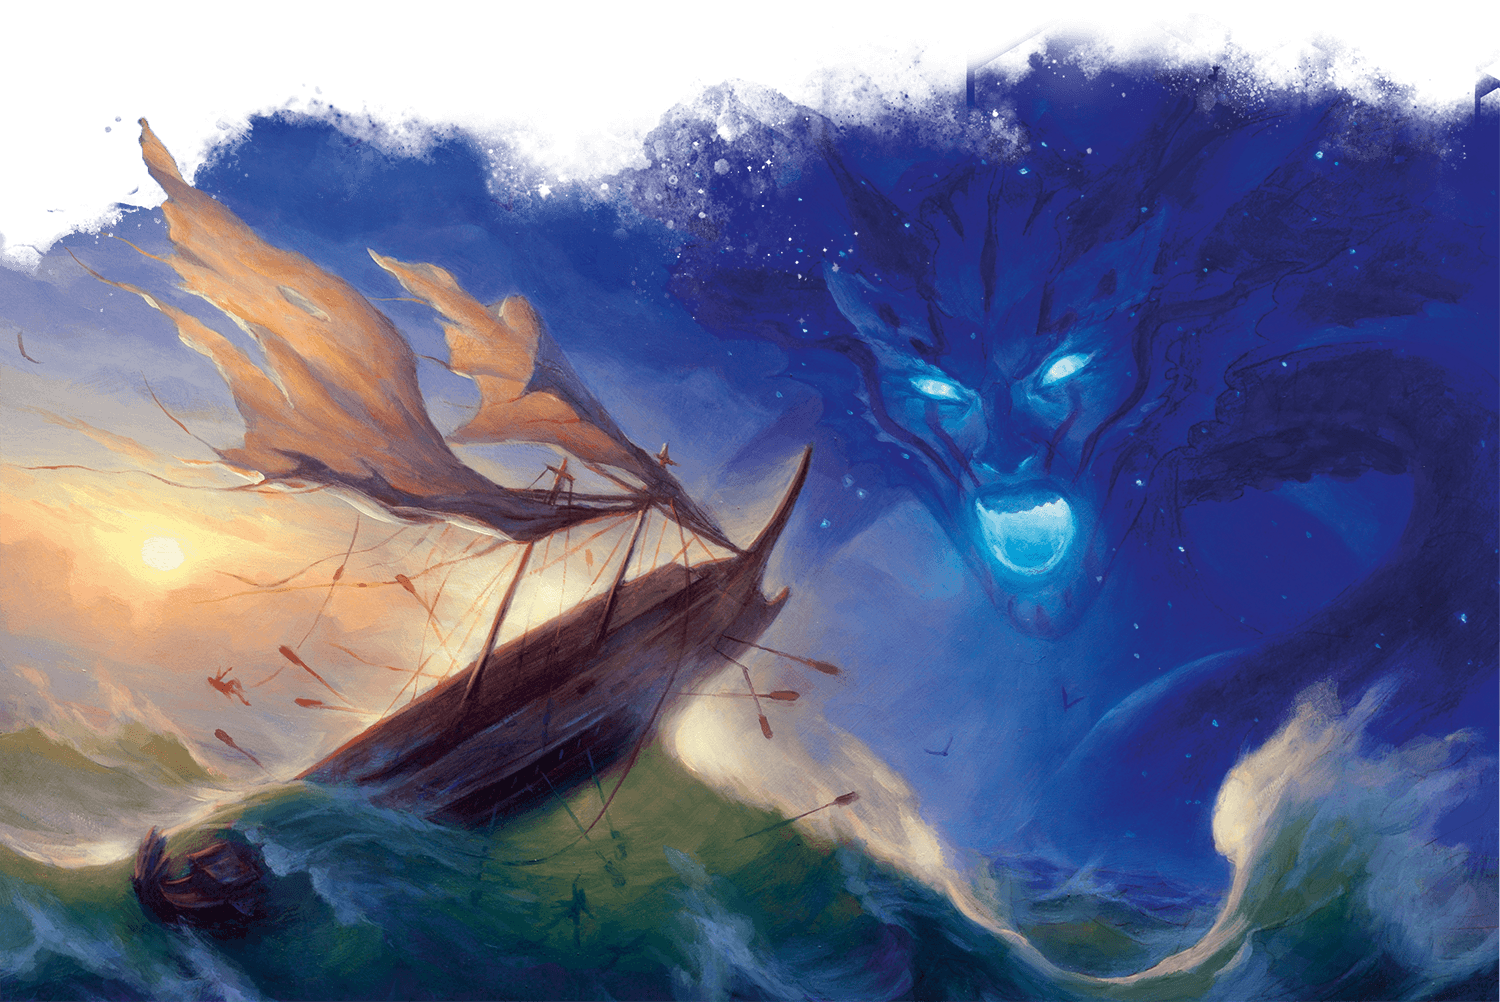
\includegraphics[width=\pdfpagewidth]{03mechanics/img/30thassaangry.png}};
    \end{tikzpicture}

